\documentclass[runningheads,a4paper]{llncs}
\usepackage{tcolorbox}
\usepackage{bbold}
\usepackage{bm} 
 \usepackage{ulem}
\usepackage{amsmath}
\usepackage{amssymb}
\setcounter{tocdepth}{3}
\usepackage{graphicx}
\usepackage{subfig}
\usepackage{url}
\usepackage{scalefnt}
\usepackage{wrapfig}
%\urldef{\mailsa}\path|{alfred.hofmann, ursula.barth, ingrid.haas, frank.holzwarth,|
%\urldef{\mailsb}\path|anna.kramer, leonie.kunz, christine.reiss, nicole.sator,|
%\urldef{\mailsc}\path|erika.siebert-cole, peter.strasser, lncs}@springer.com|    
\newcommand{\keywords}[1]{\par\addvspace\baselineskip
\noindent\keywordname\enspace\ignorespaces#1}

\begin{document}
 \scalefont{0.95}
\newcommand{\todo}[1]{\textcolor{red}{\textbf{#1}}}
\newcommand{\ori}[1]{\textcolor{purple}{\textit{#1}}}

\newcommand{\towrite}[1]{\textcolor{blue}{\textbf{#1 \\ .................. }}}
\newcommand{\torewrite}[1]{\textcolor{red}{{#1}}}
\newcommand{\toremove}[1]{\textcolor{blue}{-text removed-}}
\mainmatter  % start of an individual contribution

% first the title is needed
\title{\LARGE \bf
Multi-Modal Intention Prediction With \\Probabilistic Movement Primitives. }

% a short form should be given in case it is too long for the running head
\titlerunning{Multi-modal Intention Prediction With ProMPs}


\author{Oriane Dermy$^{1}$ %
%\thanks{This work was supported by the European Projects CoDyCo (FP7, n.600716) and An.Dy (H2020, n.731540).}%
\and Francois Charpillet$^{1}$ \and  Serena Ivaldi$^{1}$}
\authorrunning{Multi-modal Intention Prediction  With ProMPs}


% <-this % stops a space
\institute{$^{1}$ INRIA, 615 Rue du Jardin botanique, 54600 Villers-lès-Nancy\\
 name.surname@inria.fr}%


\toctitle{Multi-modal Prediction Of Intention With ProMPs}
\tocauthor{Multi-modal prediction}
\maketitle

\begin{abstract}

This paper proposes a method for multi-modal prediction of intention based on a probabilistic description of movement primitives and goals.
We target dyadic interaction between a human and a robot in a collaborative scenario. The robot acquires multi-modal models of collaborative action primitives containing gaze cues from the human partner and kinetic information about the manipulation primitives of its arm.
We show that if the partner guides the robot with the gaze cue, the robot recognizes the intended action primitive even in the case of ambiguous actions. Furthermore, this prior knowledge acquired by gaze greatly improves the prediction of the future intended trajectory during a physical interaction.
Results with the humanoid iCub are presented and discussed.


%This paper addresses the problem of allowing a robot to infer and follow trajectories decided by a partner, without requiring him to give explicit instructions.
%%him to do efforts to be understood. 
%This study encompasses two challenges.
%%that are classically handle separately: 
%First the multi-modal inference (from visual and physical interaction) facilitate the robot utilization with a robust inference skill. Second the movement primitive learning allows the robot to achieve the task precisely according to the user's intention.
%To do so, we use Probabilistic Movement Primitives (ProMPs). This method allows the robot to adapt its movement to the early-trajectory specificities. We test our approach with an experiment on the iCub robot, where it first uses physical or visual information 
%%to grasp objects correctly (then the user can determine what to do with this object) and second it uses visual information 
%to move and put the object on the position intended by the partner. Results show that the physical guidance allow the robot to adapt the learned movement efficiently and visual guidance allows to find the correct trajectory to perform. 
%%The major contribution of this study is to allow a robot to do any cooperative movements after kinesthetic teaching, where it knows when and how to act in a natural process that is to remain attentive to its partner's guidance and gaze.

%The abstract should summarize the contents of the paper and should
%contain at least 70 and at most 150 words. It should be written using the
%\emph{abstract} environment.
\keywords{multi-modality, probabilistic movement primitive, human robot interaction, collaboration}
\end{abstract}

\section{Introduction}

Les humains ont développés des compétences très développées en ce qui concerne la prédiction et l'adaptation de leurs actions lorsqu'ils sont en collaboration. Pour cela, ils utilisent des indices multi-modales (auditif, visuel, etc.) leur permettant de prédire l'intention de leur partenaire de manière robuste~\cite{walker1997infants}.


Pour collaborer efficacement avec les humains, sachant que ceux-ci exhibent des compétences anticipatives, les robots doivent aussi être capable de prédire l'intention de leur utilisateur. La prédiction de l'intention de l'utilisateur, basé sur ses mouvements implique que ces mouvements soient à la fois \textit{lisible} et \textit{prédictible}. En effet, ces conditions sont nécessaire pour que le robot puisse rapidement inférer le but du mouvement et la continuation du mouvement. 
Ici, nous défendons l'idée qu'en utilisant des informations multimodales~\cite{dillmann2004armar,weser2006multimodal}, la qualité de prédictions du robot peut être améliorée.


Dans l'étude précédente~\cite{oriane2017}, nous adressions le problème de prédire le future de trajectoires du bras du robot, initiées physiquement par l'utilisateur en interaction avec ce bras. Pour cela, la méthode ProMPs~\cite{paraschos2013probabilistic} était utilisée afin d'apprendre des primitives de mouvements à partir d'un set de démonstration ; puis de calculer la trajectoire attendue par l'utilisateur, à partir de l'observation partiel d'un mouvement initié par l'utilisateur.

Dans ce papier, nous ajoutons la modalité visuelle au robot, afin qu'il prédise l'intention de son partenaire à partir de mesures visuelles et cinématique. L'intention est ici modélisée comme la combinaison d'un but positionnel à atteindre, et d'une trajectoire que le robot doit effectuer avec son bras.

Cette fois ci, le robot apprend la combinaison de mesures sur la cinématique de son bras, lorsque son utilisateur le déplace, ainsi que le mouvement du regard de ce dernier. Ces mesures permettent ainsi au robot d'apprendre des ProMPs multi-modal, qui calcul une distribution à partir des démonstrations de chaque trajectoire.

A partir de l'inférence physique, le robot est capable de reproduire le mouvement, ainsi que de continuer un mouvement initié par le partenaire, et ce même avec peu d'observations. A partir de l’inférence visuelle, le robot est capable de prédire et d'effecteur la tache, pour des tâches ne nécessitant pas que l'utilisateur adapte la trajectoire en guidant le début du mouvement. De plus, l'inférence visuelle permet au robot de désambiguïser facilement des primitives dont le début de mouvement est similaire.
%. Moreover, this inference solves the issue of trajectories initiated similarly. 
 

%Recently, a improvement of a lot of human works consists on using robots in physical collaboration with humans. For example in assembly line, robots can help workers by doing tasks that require strength, or in hospital to help nurses to carry patients. 
%Such robots have to predict
%A critical ability for robots to collaborate with humans is the prediction of 
%their partner intention to ensure safety, efficiency and task reliability in the collaboration. 
%Some researches focus on physical measurements~\cite{oriane2017} to predict human intents. However, by measuring only physical information during the early-trajectory, robots cannot differentiate motions that begin identically. Moreover users can be reluctant to touch robots. Other researches focus on visual measurements, with human's gaze estimation but these measurements are not accurate enough for complicated tasks.
%Gathering information for predicting the user's intention during interaction given by different modalities, such as touch (gesture), sight (gaze ~\cite{meltzoff2007eyes,macrae2002} or facial expressions~\cite{bretherton1991intentional,gergely1999early}), etc. make the robot utilization easier.
%In daily life, humans use multi-modal cues (hearing, sight, etc) to predict the intent of their partner in a robust way~\cite{walker1997infants}.
%,stivers2005introduction 
%Similarly, robots prediction abilities can be improved by using multi-modal information (\cite{dillmann2004armar,weser2006multimodal}).
%In this paper, both visual and physical measurements are used to predict the human intent. This intent is modeled as a goal location and a trajectory that the robot has to perform with its arm.
%, followed by a corresponding task (such as grasp or place objects). 
%Physical (robot's arm) and visual (partner's gaze) motions are learned using a method called Probabilistic Movement Primitives (ProMPs\cite{paraschos2013probabilistic}), that are distributions other trajectories. From the physical inference, the robot is able to repeat movements and to continue movements initiated by the partner, even with few early-observations. From visual inference the robot performs tasks that didn't require the partner guidance to refine the expected trajectory. Moreover, this inference solves the issue of trajectories initiated similarly. 


\begin{figure}[t]
\centering
 \subfloat[Visual Guidance.]{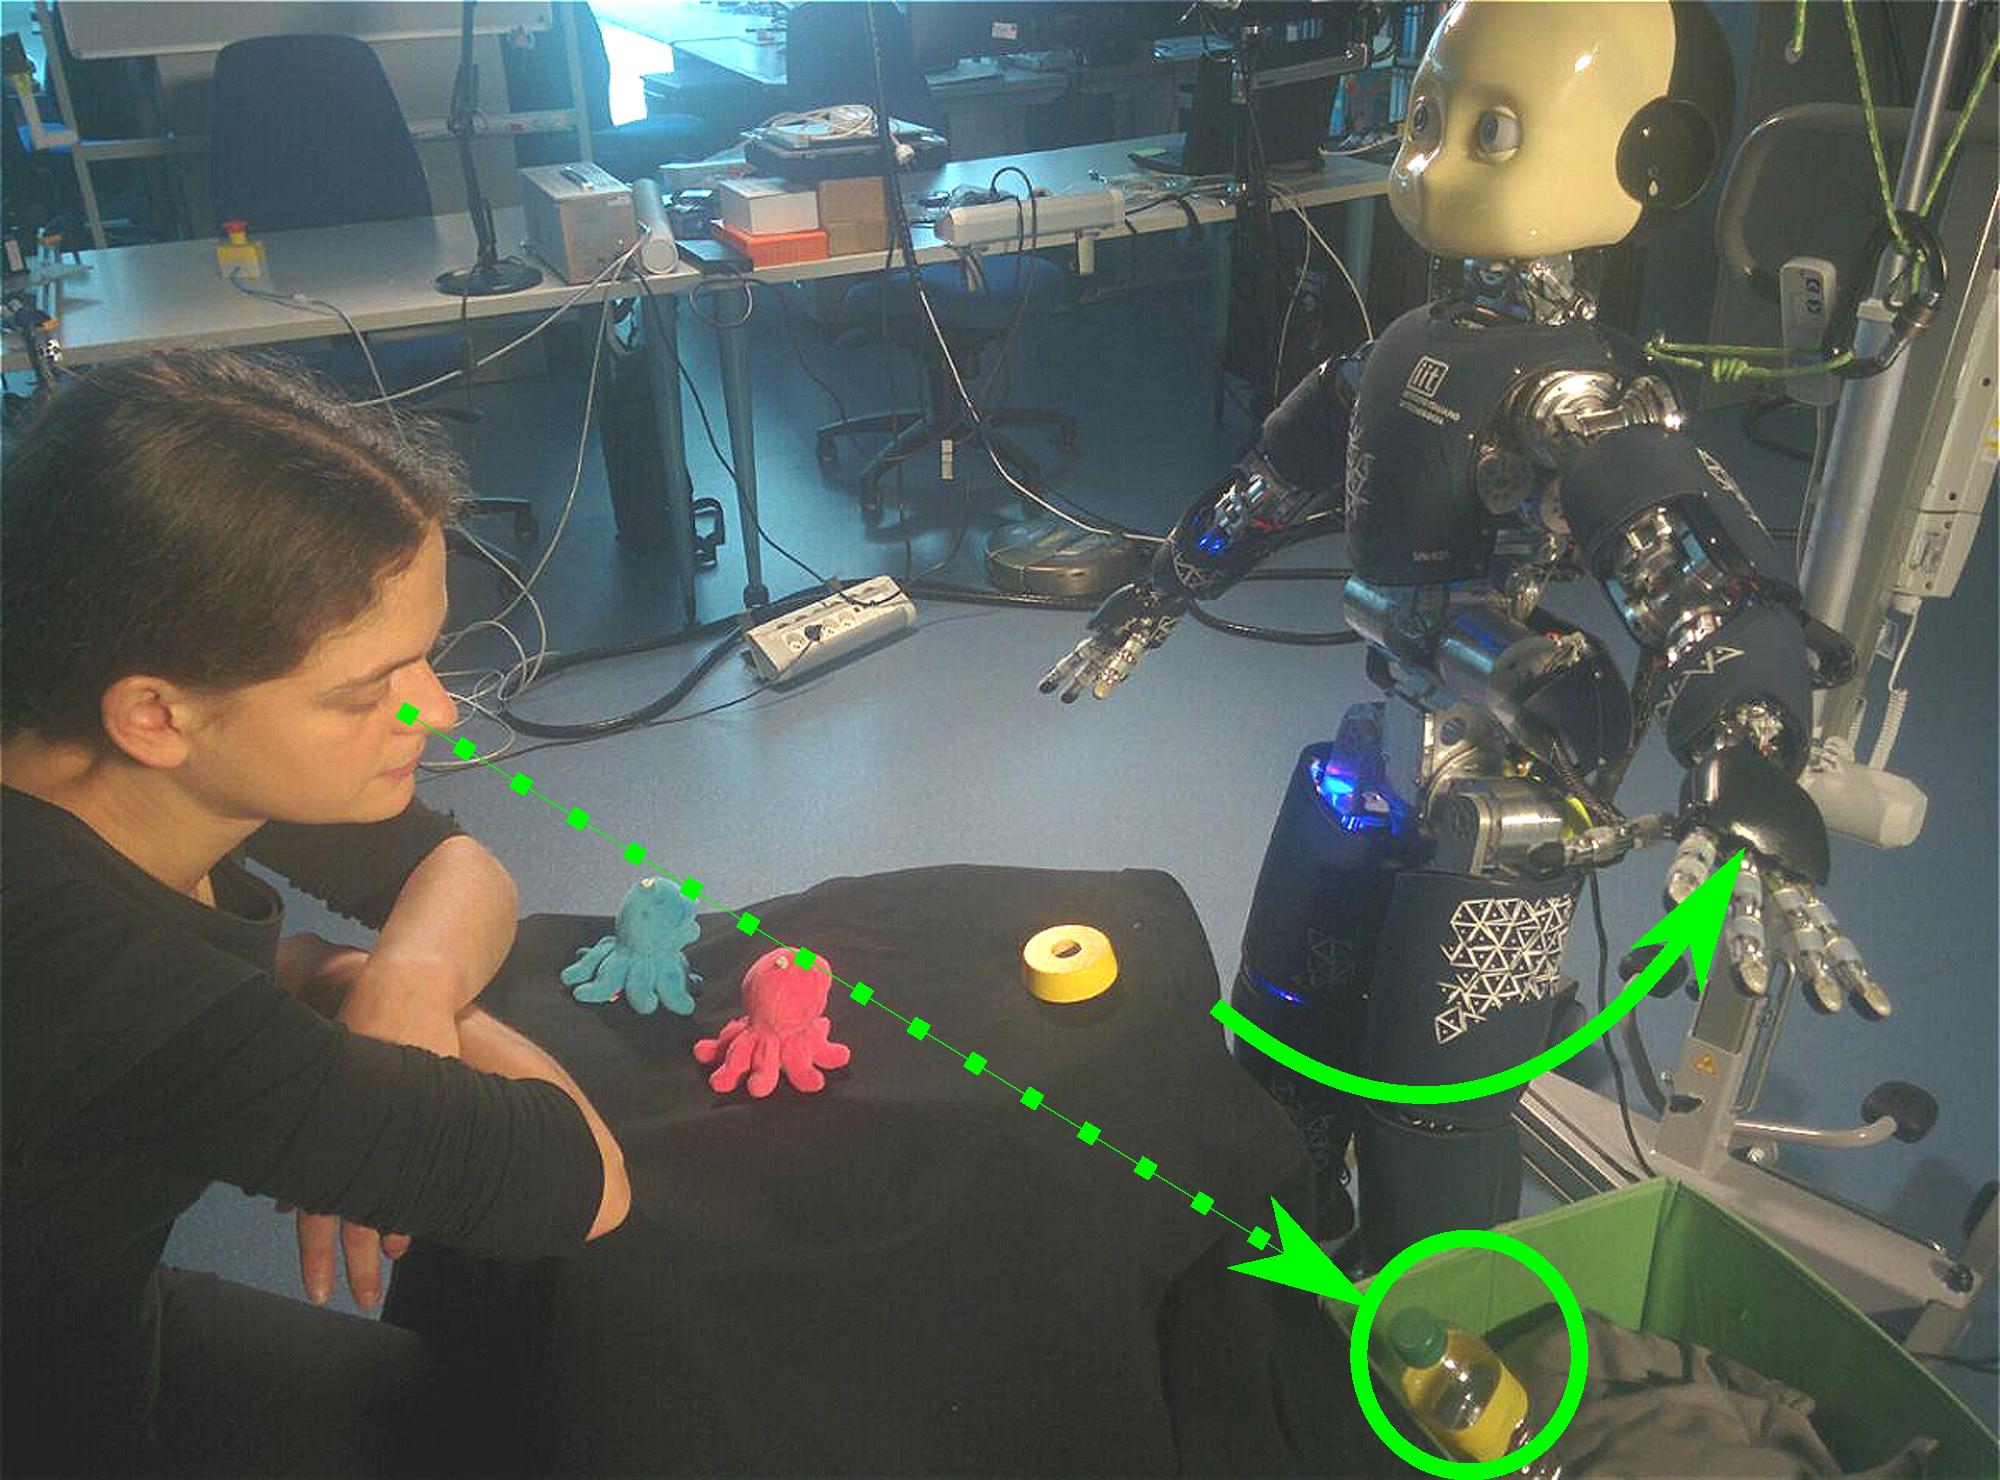
\includegraphics[height=3cm]{figures/fig1_bV2.pdf}}
 \subfloat[Physical Guidance.]{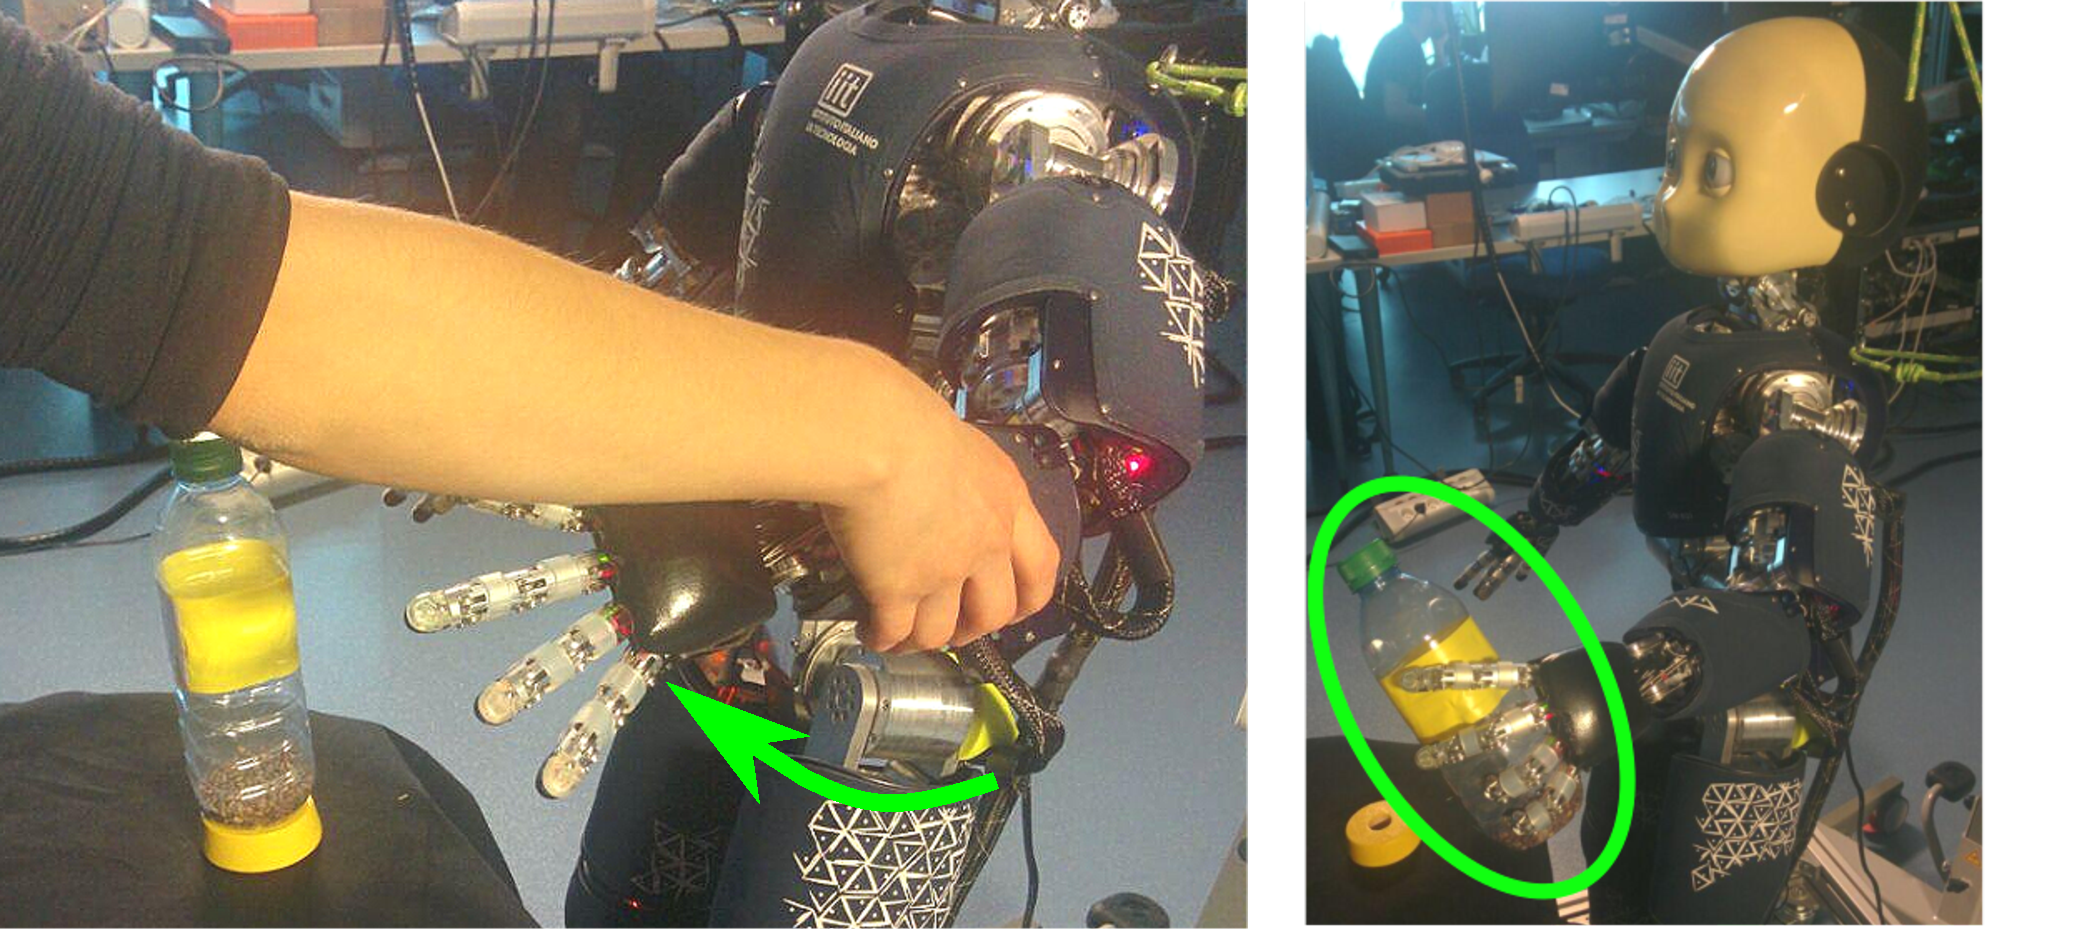
\includegraphics[height=3cm]{figures/fig1_aV2.pdf}}
\caption {The humanoid robot iCub a) recognizes the intended movement primitive using the partner's directional gaze; b) predicts the movement to perform using the partner's physical guidance at the beginning of the movement.}
\label{fig:idea}
\end{figure}


%The visual inference is can be considered as a prior allows our robot to continue correctly and autonomously a trajectory initiated by its partner.

%In our previous work, the human intent was  \footnote{the first data of the trajectory initiated by the partner}. 
%Therefore, we add the visual modality to give a prior expectation of the partner's will, to avoid the previous issue and to improve the inference robustness. To do so, the robot computes the likelihood that each ProMP (links to a goal position area) corresponds to the partner's head orientation, after having learned the correlation between the different goal positions and partner's head orientations.
%The partner's head orientation is retrieved by the iCub's eyes (camera) and the Intraface software\todo{citation}.
%The contribution of this paper involves using the human's gaze orientation as a prior probability of the possible goal locations
%Therefore in this paper, we provide our robot with a second modality: the sight. To do so, our robot can now perform the physical trajectory expected by its partner using the user's gaze trajectory. 
%
%A conceptual representation of the problem is shown in Figure~\ref{fig:conceptual}.
%In the upper part of this figure, we represent the training step for one movement primitive 
%%(let us call it $k$)
%, where our robot is guided by the user to perform a certain task several time
%% (for example $N_k$)
%. From these demonstrations, our robot collects a set of "entire demonstrations". Both kinematics (Cartesian positions) and dynamics (wrenches) and visual (partner's head orientation) information are collected. The 
%%$N$ 
%trajectories constitute the base for learning the  
%%$k-th$ 
%primitives (prior distribution.)
%%, that is learning the parameters $\boldsymbol{\omega_k}$ of the trajectory distribution. We call this learned distribution the \textit{prior distribution}. This $k-th$ ProMP is also associated with the user's head's orientation when he looks at the goal position. To do so, $n_{gaze}$ samples of the Euler angles of the user's head orientation are recorded. A normal distribution $\boldsymbol{h\_\omega_{k}}$ is then computed from these samples, and the robot learns the association $\{\boldsymbol{\omega_k}, \boldsymbol{h\_\omega_{k}}\}$ 
%%Then the process is replicated such that we have one ProMP for every task. 
%% $N$ demonstrations of this movement are provided. From these demonstrations, the robot computes a model of the movement using the ProMP method, by computing the distribution of the model's parameter $\boldsymbol{\omega}$. We call this learned distribution the \textit{prior distribution}. 
%The bottom of the figure represents the inference steps. First, the user initiates physically the robot's hand movement and the robot finishes the movement to grasp the object. Second, the user does the expected trajectory with its head, then the robot follows this trajectory to drop the objects. To present the improvement with our previous work, the learned trajectories of the dropping phase have identical initial and final positions (thus, the physical recognition from the early observations is harder).
%%From the head orientation of the user, the robot detects probabilistically  when the user is looking at a goal position. When this detection is perform, the robot identifies the corresponding ProMP to follow. From the early observations of a movement initiated by the human partner, the robot can then estimates the future trajectory, given the early observations (\textit{e.g.} first portion of a movement) and the prior distribution (that is the identified ProMP). To do so, it computes the parameters $\boldsymbol{\omega}^*$ of the \textit{posterior distribution}. The corresponding trajectory can be used by the robot to autonomously finish the movement, without relying on the user.
% %it updates the ProMP to by-pass\todo{??} by the early observations: this posterior distribution is used by the robot to finish the movement.
%\towrite{What we do to show that it is a good approach, experiments}
%It has been tested  with the robot iCub. To do so, the human operator simply grabs the robot's forearm and the robot uses its own eyes to retrieve visual information.
%Thanks to the Cartesian position information, the robot can continue movements autonomously, without being guided by the human\footnote{
%Notably, in previous studies~\cite{paraschos2015model}, ProMPs were used to learn movement primitives using joint positions. Here, we use Cartesian positions instead of joints positions, to exploit the redundancy of the robotic arm in performing the desired task in the 3D space. 
%As for the forces, we rely on a model-based dynamics estimation that exploits the 6 axis force/torque sensors \cite{ivaldi2011computing,fumagalli2012force}.
%}.
%\todo{add forces info if we have done it} 
%Thanks to the force information, the robot can detect if the user's forces are larger than the ones it has previously learned: in this case, the robot assumes that the current movement is probably a new demonstration of a new primitive (\textit{e.g.}, a new task, different from the one previously learned) and then instead of trying to guess the goal using the information of the previous primitive, it can follow the users' movement to learn a new movement primitive.
%To summarize, the contributions of this paper are a creation open-source of a framework\cite{multi-ProMP:2017} that allows a robot to predict the movement and action to perform, thanks to visual or physical observations, and a study about this inference that shows that the movements can be more accurate with physical measurement, but that the visual inference allows a correct movement recognition with less effort for the human partner. This study is an improvement of our previous work~\cite{oriane2017}.
The paper is organized as follows. 
%\towrite{To rewrite the following paragraph to adapt it to the current paper.}
We briefly report on the literature about intention prediction and gaze as a conveyor of intention information in Section~\ref{sec:SOA}.
% reviews the literature on intention prediction, gaze as a conveyor of intention information, and physical interaction. 
 Section~\ref{sec:pblm} formulates the problem settled in this paper.  Section~\ref{sec:learningPROMP} summarizes the theoretical basis of the ProMP method to learn movement primitives, applied to learning multi-modal information. Section~\ref{sec:xp} presents a multi-modal intention recognition application, where results about the action recognition improve the prediction of the future trajectory.
%In section \ref{sec:video} provides the links to the videos showing how to use the software in simulation and on the iCub.
Finally, section~\ref{sec:ccl} discusses the proposed approach, its limitations and outlines our future developments.

\section{Related Works}
\label{sec:SOA}
%\towrite{Follow the structure that you cited in the introduction if possible. What are the main techniques to solve the problem? Are there papers more focusing on the application? Are there papers more focusing on the theory? Are there different techniques? Here we need to come up to around 20 papers to cite }
%To predict the trajectory to perform, 

Pour déterminer la trajectoire à effectuer, le robot doit inférer l'intention de son partenaire. Ici, nous nous intéressons à l'inférence effectuée à partir d'indices physiques et visuels. Les paragraphes suivants fournissent un résumé de la litératures des différentes études concernant la prédiction de l'\textit{intention} et du \textit{regard}. En ce qui concerne l'état de l'art sur les  \textit{primitives de mouvements} et \textit{l'inférence durant l'interaction physique homme-robot}, nous nous referons à~\cite{oriane2017}.
%\todo{Formalizing intention and prediction of intention}
\paragraph{Intention} 
Prédire l'intention d'un humain signifie essentiellement prédire le but de son action en cours ou arrivant, ainsi que prédire le mouvement permettant d'atteindre le but visé.
%. The 
%action, i.e., the 
%movement performed to reach the goal should also be predictable. 
%Dragan et al. formalized the difference between predictability and legibility in \cite{Dragan2013rss}.
La compréhension de l'habilité à prédire l'intention intéresse différents domaines : l'analyse de l'interaction entre humains~\cite{meltzoff2007eyes,bretherton1991intentional}; les études cherchant à rendre le comportement des robots compréhensible par les humains~\cite{kim2017collaborative,dragan2014integrating}; ou encore les études cherchant à rendre les robots capables de comprendre l'intention des humains. Notre étude se situe dans ce derniers cas, comme beaucoup d'autres applications, tels que les études mettant en jeu une collaboration homme-robot~\cite{ferrer2014bayesian,wang2012probabilistic}, ou encore pour la navigation robotique~\cite{mitsugami2005robot}. Ici, le regard de l'utilisateur est utilisé comme un indice essentiel permettant permettant de déterminer l'intention de l'utilisateur, couplé avec la direction du regard de l'humain et avec ses actions associées\todo{reformuler}

%macrae2002,baron1997build,
%, or by analyzing model through robotics such as in~\cite{pitti2013modeling}, \textit{etc.})
%, to improve the interaction
%,HuangHAD17
%, for improving programs \cite{bader2009multimodal}
\paragraph{\label{sec:gazesoa}Gaze as a conveyor of intention information}

%In human-human interaction, gaze following is an important skill.
La direction du regard les l'indice le plus fondamental utilisé lors d'interaction sociale, car il permet d'avoir une attention conjointe entre les partenaires.
%Thus, a lot of research study this ability. 
%In human-human interaction, a study~\cite{brooks2002importance} show that 12 months old children can already follow the gaze of an adult and engage joint attention. %Some studies try to model the gaze following and joint attention to understand better the human-human interaction.
%In~\cite{friesen2011gaze}, they introduce a Bayesian model where gaze following occurs as a consequence of goal inference in a learned probabilistic graphical model.
%proactive, reactive and tracking gaze behavior [5].
%We focus in this work on Human-Robot Interaction studies, where 
En effet, beaucop d'etudes prennent en compte la direction de la tête/du regard humain afin d'intéragir avec celui ci.
%\ori{We might have to compress this part}
%\begin{itemize}
%\label{hri-goal}
%\item to analyze the human-robot interaction~\cite{ivaldInitiative2014};

Certains utilisent cette direction afin d'estimer l'engamenet de l'utilisateur avec le robot companion~\cite{castellano2009detecting,anzalone2015evaluating,ivaldi2017towards};
%~\cite{ishii2011combining}~\cite{Ivaldi2015}
%, they study the user's gaze during human-robot interaction and they show that if the robot takes the initiative during the learning of a collaborative task then, after learning, the rythm of the interaction is faster and, by using a simple joint attention mechanism, the user's perceived the robot as engaged and they were globally able to read the behavior of the robot. 
%\item 
ou d'estimer l'émotion de l'utilisateur afin de corriger le comportement du robot~\cite{boucenna2014robot}.
%Notably, in \cite{ishii2011combining}, they show that the duration of gaze is a strong predictor of user's engagement and the distance of eye movement and pupil size are useful in estimating the conversational engagement. that is also linked to the negative attitude towards robots~\cite{Ivaldi2015} ("the more people have a negative attitude towards robots, the less they tend to look at the robot's face").;
%\item 
D'autres améliore le comportement du robot en assurant la sûreté de l'interaction~\cite{traver2000making};
%, where they use human's gaze not to predict the intent of the human but to estimate if the human perceives the robot, to adapt the robot's behavior and thus, to ensure safety.
en anticipant l'action de leur partenaire~\cite{huang2016anticipatory};
%, where the robot uses this anticipation to pro-actively perform a task. This work is based on an anticipatory control method, results show that by using this proactive control instead of a reactive one, the user completes the collaborative task faster. A limitation of this work is that the gaze tracking requires the user to wear a pair of SMI Eye-Tracking Glasses.
%\item to improve software as in~\cite{bader2009multimodal} where an interface recognizes the gesture of the user's hand by using a multi-modal integration model of natural gaze behavior. To do so, they first study the human's gaze during a gesture task, and then they improve the interface.
%\item 
%to control robots navigation~\cite{mitsugami2005robot};
% , the user just gaze at one robot and then gaze at the destination on the floor. To do so, they use an EMR-8 eye mark recorder (NAC inc.) and they use a method called "corneal reflection-pupil center" from which they compute the eye direction in real-time.
%\item 
ou en adaptant les actions du robot aux intentions de son partenaire~\cite{kozima2001robot}.
%, they use an epigenetic model from which an infant-like robot empathetically understand the partner's behavior. To do so, a robot learns to correlates goals (or intention) with behaviors. 
Ce dernier cas correspond à nos objectifs actuels.
%, where our robot has to act according to it partner's expectation.

Pour compléter cet objectif, nous calculons d'abord l'orientation de la tête/du regard du partenaire.Pour ce faire, différentes méthodes existent telles que, %(\cite{heinzmann19983}).
Les Réseaux de Neurones~\cite{baluja1994non} % where they use them in a non-intrusive way to track the user's gaze with a precision of $1.5$ degrees. Another possibility is to use
, le calcul de gradients~\cite{timm2011accurate}%, where they localize precisely the center of the eyes. 
%Their program is available on Github\footnote{\url{https://github.com/iitmcvg/eye-gaze}}. 
,  ou en utilisant les probabilités. Le regard est souvent utilisée en tant qu'à priori sur la tâche voulu du partenaire (\textit{e.g}, our work with ProMPs)
%, they use a probabilistic model of gaze imitation and shared attention. They estimate the gaze vector to detect the most likely object being looked at by the user. 
%Like in our current work, 
%They also use the gaze as an apriori, 
to detect the object of interest (\textit{e.g.},~\cite{HOFFMAN2006299} with Neural Networks)
%, us to perform the expected behavior. 
, or to predict the goal location (\textit{e.g.},~\cite{chaandar2016bayesian} with dynamic models). 
%also computes a prior probability based on the user's gaze direction 
%Moreover, we both compute a posterior probability of this goal location based on interacting models. 
The main differences between our study and~\cite{HOFFMAN2006299,chaandar2016bayesian} is that these works are interested in the human motion prediction while we associate human gaze to the robot motions.
%(instead of the robot's motion expectation),
%and they use other methods (Neural Networks and Dynamic models).%learn reaching motions from a contracting nonlinear dynamics model, where the non-linear function is learned through a Neural Network (whereas we use Probabilistic Movement Primitives, that has some advantages compared to dynamics models: \textit{c.f.} paragraph \textit{movement primitives}).
%; and they use extended Kalman filters to compute the posterior distribution (while we use simple Kalman filter).
% The method consist on using a convolution neural network to obtain a gaze map (e.g. a spacial map where each pixel has a probability to be the gaze point) that is linked to the position of candidate goal location. They call this technique gaze-based multiple model intention estimator (G-MMIE), and this method is more robust than previous neural networks models, called adaptive neural intention estimator (ANIE) \cite{ravichandar2015human} and multiple-model-intention estimator (MMIE)\cite{chaandar2015human}. 

%\ori{ Garde t'on cet exemple?} 
%In \cite{cristinacce2004comparison}, they implement the face tracking by using a Constrained Local model approach(CLM, \cite{cristinacce2006feature}), that uses a joint shape and texture appearance model to generate a set of region template detectors of the human face. It consist on detecting seom rectangular region around each feature that has been learned. In this study, they show their method (CLM) outperform the following other methods: Active Appearance Model (AMM \cite{edwards1998face}, where they model the whole object region and not a set of local feature templates), Template Selection Traker (TST\cite{cristinacce2006facial}), or Shape Optimised Search (SOS\cite{cristinacce2004comparison})). Although this method detects the human face, they don't use it to detect the gaze of the user. 
In some research studies, the human's gaze direction is accurately measured using 
%available devices and programs, such as 
eye tracker~\cite{ishii2011combining,mitsugami2005robot}.
%where they use glasses to have accurate human's gaze estimation,
%, they use a 3D model: The two first layers track the person face in real time, and the third layer allows to feet the 2D model to the face and to allow the derivation of the 3D pose of the head. The gaze direction is computed from the distance between the iris and the corners of the eye.
%or NAC Image Technology Eyemark Recorder model EMR-8 ( \cite{,ma2005eye}.)
%, where they use a . 
In our case, we rely on visual processing of the robot's cameras, which is less invasive and it does not require to wear a device, even though it is less accurate than eye tracker.
%\textit{Movement primitives (MPs)} This is a well-established paradigm for representing complex motor skills. In our previous paper~\cite{oriane2017}, we already give the state of the art of such methods.
%The most known method for representing movement primitives is probably the Dynamic Movement Primitives (DMPs~\cite{ijspeert2013dynamical,schaal2006dynamic,meier2016probabilistic}). DMPs use a stable non-linear attractor in combination with a forcing term to represent the movement. The forcing term enables to follow specific movement, while the attractor asserts asymptotic stability. 
%In a recent paper, \cite{meier2016probabilistic} proposed an extension to DMPs, called PDMP (Probabilistic Dynamic Movement Primitive). This method improves DMP with probabilistic properties to measure the likelihood that the movement primitive is executed correctly and to perform inference on sensor measurement. However, The PDMPs do not have a data-driven generalization and can deviate arbitrarily from the demonstrations. This last difference can be critical for our applications with the humanoid robot iCub, since uncertainties are unavoidable and disturbances may happen frequently and de-stabilize the robot movement (for example, an unexpected collision during the movement). Thus, the ProMPs method is more accurate for our software.
%
%\cite{ewerton2015learning}, \cite{paraschos2013probabilisticTrajectory} and \cite{maeda2014learning} 
%%\todo{I don't find this paper on the internet, so I cannot cite it. Can you give me the bibtex?} 
%compared ProMPs and DMPs for learning primitives and specifically interaction primitives. 
%%With the DMP model, at the end of the movement, only a dynamic attractor is activated. Thus, it always reach a stable goal. 
%%The properties allowed by both methods are temporal scaling of the movement, learning from a single demonstration, and generalizing to new final position. 
%For inferring the intention of the robot's partner, we use the ProMP method because these studies show that this method adds the ability to do inference (thanks to the distribution), to force the robot to pass by several initial via-points (the early observations), to know the correlation between the input of the model, and to co-activate some ProMPs.
%% Specifically, we use the ProMP's conditioning operator to adapt the learned skills according  to observations. The ProMPs can encode the correlations between forces and positions and allow better prediction of the partner's intention.
%
%In our study, we need these features, because the robot must determine a trajectory that passes by the early observations (beginning of the movement where the user guides physically the robot). 
%
%
%Other methods can be used to obtain movement primitives. A hierarchy of neural networks~\cite{billard2001learning}, based on Recurrent Neural Networks (RNN) can be used aiming to simulate a human brain; Hidden Markov Models (HMM introduced for movement skills in~\cite{fine1998hierarchical}) can categorize movements, represent a movement temporal sequence or recognize human behavior~\cite{nguyen2005learning}; Gaussian Mixture Models can encode the relationship between variables of movement primitives, like in where they combine GMM with  Gaussian Mixture Regression (GMR) to reproduce learned tasks; \textit{etc.}

%%%%%%%%%%%%%%%%%%%%%%%%%%%%%%%%%%%%%%%%%%%%%%%%%%%%%%%%%%%%%%%%%%%%%%%%%%%%%%%%
\section{Formulation du Problème}
\label{sec:pblm}
\begin{figure}[t]
\centering
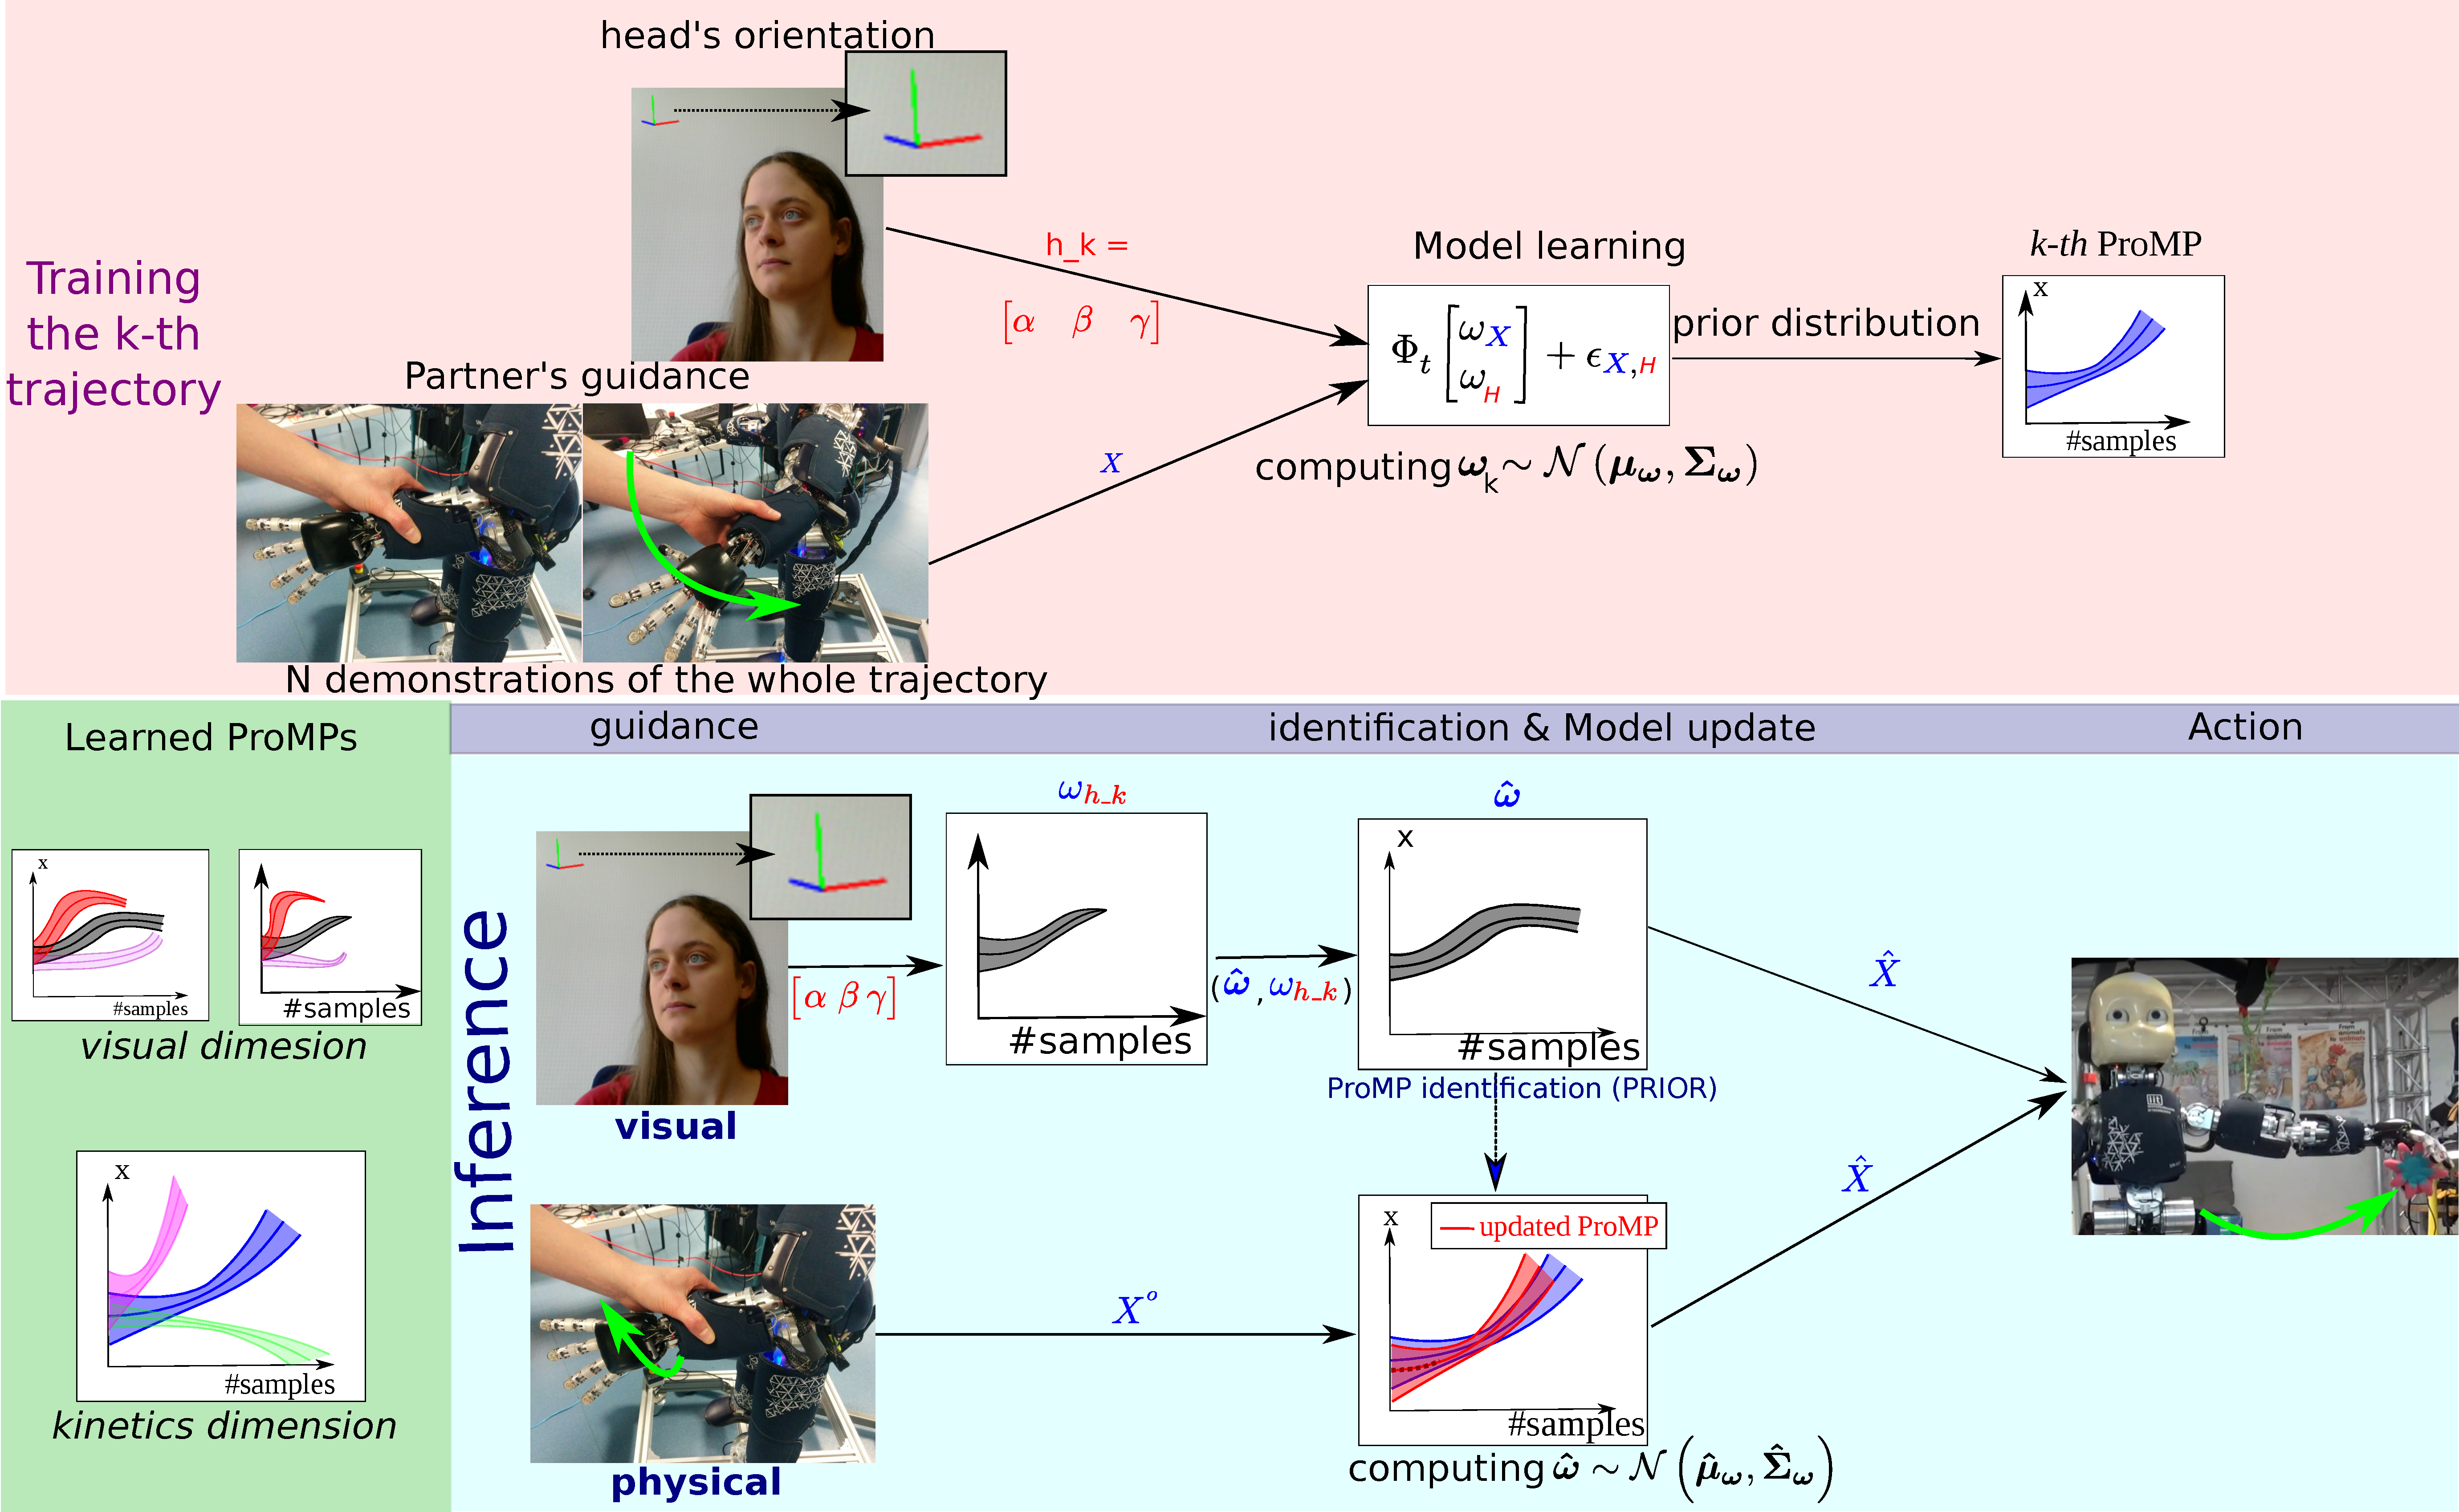
\includegraphics[width=\hsize]{figures/conceptualV2.pdf}
\caption{Utilisation conceptuelle des \textit{ProMPs} afin de prédire la trajectoire que l'utilisateur souhaite que le robot exécute. Lors de la phase d'apprentissage (en haut), les \textit{ProMPs} sont apprises à partir de trajectoire de démonstration d'un utilisateur. Lors de la phase d'inférence (en bas), le robot reconnaît la \textit{ProMP} correspondant à la trajectoire initiée par le partenaire, à l'aide de mesures visuelle ou haptique.}
\label{fig:conceptual}
\end{figure} 
Ce papier présente une méthode de prédiction multi-modale de l'intention, basée sur une description probabiliste de primitives de mouvement et de buts.
Le scénario d'utilisation visé consiste en des interactions dyadiques entre l'humain et le robot, interactions qui peuvent être à la fois visuelles et haptiques. Afin de présenter cette méthode, des expériences sont réalisées, qui consistent à des déplacements d'objets (\textit{c.f.} Figure~\ref{fig:idea}), en suivant des trajectoires différentes. 
%The process is as follows. an object to inspect is placed in front of the robot. First, 
Pour cela, l'utilisateur du robot choisi de le guider soit physiquement en déplaçant son bras (\textit{c.à.d.} interaction physique), soit en présentant le trajectoire à effectuer à l'aide de mouvement de tête (\textit{c.à.d.} interaction visuelle). Le robot doit alors utiliser cette information pour continuer le mouvement par lui-même.
%initiates a movement physically moving the robot, to allow it to understand how to grasp the object. After the inspection, 
Lorsque l'utilisateur guide visuellement le robot, celui-ci suit l'orientation de la tête de son partenaire afin d'en déduire l'intention sous-jacente. Pour cela, le robot identifie, parmi celles apprises, la primitive de mouvement correspondant le plus à la trajectoire du regard du partenaire. À l'aide de cette identification, le robot prédit alors la tâche qu'il doit exécuté (en effet, à chaque primitive correspond une tâche à effectuer).

 The robot predicts then the current task and the future intended movement. It completes the intended task by placing the object in the expected place, following the trajectory intended by the partner. During physical guidance, the user starts to physically move the robot to perform the action; after early observations, the robot predicts the future movement to perform. If the human partner uses both modalities, the movement primitive can be recognized from the visual guidance (prior) and physical guidance can be used to refine the predicted trajectory (posterior). 
%box (box A or box B). \todo{to adapt according to our trajectory.} 
To realize this scenario, we make several hypotheses. 
%We use the ProMP method to predict the partner intention instead of pre-programming the robot since its behavior depends on the partner's intent. 
Tracking the gaze using the eyes direction is difficult because of saccadic eye movement directed towards the goal, that could cause the gaze trajectory to be inconsistent. Therefore, the partner's head orientation is used to determine his intent. We assume the user's position with respect to the robot is almost fixed during the learning and the recognition task, because the robot learning is dependent on the partner's head orientation. We assume that the partner's head orientations when he/she looks at a same goal follow a normal distribution. 
%From our measurements, we assume the partner's head orientation measurements are not accurate. This assumption allows the posterior distribution of a ProMP to be computed correctly, without forcing this new distribution to by-pass roughly via the observed data (see \ref{fig:infgaze}).\todo{voir avec Serena}
%\sout{The technical implementation is outlined in Fig.~\ref{fig:conceptual}.
%In a first step, off-line, the human teaches the appropriate actions to be executed for the different goals and objects, using programming by demonstration. From a set of recorded movements, we compute a generalized representation of the action using Probabilistic Movement Primitive. Each primitive carries information about the goal and the object type. 
%In a second step, on-line, the human simply gazes at the goal for the intended action. A probabilistic model of the gaze allows to identify the most likely goal and the most likely primitive corresponding to the intended action.}

A conceptual representation of the problem is shown in Fig.~\ref{fig:conceptual}.
To learn the movement primitives (top), two partners run several demonstrations: one moves the robot's arm while another moves his head, following the trajectories to learn.
%The upper part of the figure depicts the training step for one movement primitive
%(let us call it $k$)
%, where the robot is guided by the user to perform a task several times.
% (for example $N_k$)
From these demonstrations, the robot collects the Cartesian position of its arm
%, dynamics (wrenches)
and the partner's gaze (head orientation). The 
%$N$ 
trajectories make the base for learning the  
%$k-th$ 
primitives (prior distribution).
%, that is learning the parameters $\boldsymbol{\omega_k}$ of the trajectory distribution. We call this learned distribution the \textit{prior distribution}. This $k-th$ ProMP is also  associated to the user's head's orientation when he looks at the goal position. To do so, $n_{gaze}$ samples of the Euler angles of the user's head orientation are recorded. A normal distribution $\boldsymbol{h\_\omega_{k}}$ is then computed from these samples, and the robot learns the association $\{\boldsymbol{\omega_k}, \boldsymbol{h\_\omega_{k}}\}$ 
%Then the process is replicated such that we have one ProMP for every task. 
% $N$ demonstrations of this movement are provided. From these demonstrations, the robot computes a model of the movement using the ProMP method, by computing the distribution of the model's parameter $\boldsymbol{\omega}$. We call this learned distribution the \textit{prior distribution}. 
The bottom of the figure represents the inference step. The partner follows with his/her head the robot's movement and/or he/she physically initiates the robot's hand movement. When the prediction is done, the robot finishes autonomously the movement (i.e., drop the hand-held object).
%Second, the user follows the expected trajectory with its head, and the robot follows this trajectory to place the objects.
To show the improvement with respect to our previous work, the learned trajectories of the dropping phase have identical initial and final positions (making the prediction from early observations harder, and possible here only thanks to the multimodal primitive).

%%%%%%%%%%%%%%%%%%%%%%%%%%%%%%%%%%%%%%%%%%%%%%%%%%%%%%%%%%%%%%%%%%%%%%%%%%%%%%%%
\section{Methods}

This section presents the ProMP method used to learn the motion primitives and to predict the trajectory of the ProMP given one modality. See \cite{oriane2017} for further information.

%\subsection{Notation}\label{sec:notation}
%To ease the reading and the understanding of the theoretical tools, we will use the following notations:
%
%To facilitate understanding of the theoretical framework, we first introduce the notations we use in this section and throughout the remainder of the paper.
%
%\noindent
%\textbf{Trajectories:}
%\begin{itemize}
%\item $X(t)\in\Re^6, X(t) = [x(t), y(t), z(t), o_1(t), o_2(t), o_3(t)]^\top$: the Cartesian coordinate with roll/pitch/yaw angles of the robot's end-effector.
%\item $F(t) \in\Re^2, F(t) = [n_1, n_2]^\top$: the wrenche (\textit{i.e.} force and moment) norm measured by the robot at the contact level (end-effector).
%\item $ A(t) = [a_{1}(t), a_{2}(t), a_{3}(t)]^\top$: the roll/pitch/yaw-axis of the user's head orientation computed from the Intraface software.
%\item $\xi(t) \in\Re^{11}$: the generic vector containing the current value or state of the trajectories at time $t$ (in our case the state is composed on position, orientation, wrench, and gaze direction).
%\item $\Xi = \Xi_{[1:t_{f}]} = [\xi(1), \ldots, \xi(t_{f})]^\top \in\Re^{11 \cdot t_{f}}$ is an entire trajectory, consisting of $t_f$ samples or data points. 
%
%\item $\Xi_{i[1:t_{fi}]}$ is the $i$-th demonstration (trajectory) of a task, consisting of $t_{fi}$ samples or data points. 
%
%%For example, $\Xi_{i[1:t_{fi}]}= [\xi_i(1), \ldots, \xi_i(t_{fi})]^\top $ is the $i$-th trajectory.
%
%%\item $t_{fi}$: total number of samples of a $\Xi_i$ trajectory;
%%\item $\Xi = \Xi_{[1:t_{f}]} \in\Re^{D \cdot t_{f}}$: a trajectory. For example, $\Xi_{i[1:t_{fi}]}= [\xi_i(1), \ldots, \xi_i(t_{fi})]^\top $ is the $i$-th trajectory.
%\end{itemize}
%\textbf{Movement Primitives:}
%\begin{itemize}
%\item $k \in [1:K]$: the $k$-th ProMP, among a set of $K$ ProMPs that represent different tasks/actions. 
%\item $n_k$: number of recorded trajectories for each ProMP.
%\item $S_k = \{\Xi_{\{k,1\}},\ldots,\Xi_{\{k,n_k\}}\}$: set of $n_k$ trajectories for the $k$-th ProMP. 
%%For clarity, we consider $\Xi_i \equiv \Xi_{\{k,j\}}$.
%\end{itemize}
%\begin{itemize}
%\item $\xi(t) = \Phi_t \boldsymbol{\omega} + \epsilon_\xi$ is the model of the trajectory with:
%\begin{itemize}
%\item $\epsilon_\xi \sim \mathcal{N}(0, \beta)$: expected trajectory noise.
%\item $\Phi_t \in \Re^{11\times 11 \cdot M}$: It is a block diagonal matrix of M radial basis functions (RBFs) used to model trajectories, with:
%
%$ \psi_{ji}(t) =\dfrac{e^{-(t - c_i)^2 \over 2h}}{\sum_{m=1}^{M} e^{-(t - c_m)^2 \over 2h} }$: $i$-th RBF for all inputs $j \in [1:11]$. 
%
%It must be noted that the upper term comes from a Gaussian $\frac{1}{\sqrt{2\pi h}} e^{-(t - c_i)^2 \over 2h}$, where $ c_i, h$ are respectively the center and variance of the $i$-th Gaussian. In our RBF formulation, we normalize all the Gaussians.
%ˆ%\item[-] $ c_i, h$: center and variance parameters of the $i$-th Gaussian.
%\item $\boldsymbol{\omega} \in\Re^{11 \cdot M}$: time-independent parameter vector weighting the RBFs, \textit{i.e.}, the parameters to be learned.
%
%\end{itemize}
%
%\item $p(\boldsymbol{\omega}) \sim \mathcal{N}(\mu_{\boldsymbol{\omega}}, \Sigma_{\boldsymbol{\omega}})$: normal distribution computed from a set $\{\boldsymbol{\omega}_1, \ldots, \boldsymbol{\omega}_n\}$. It represents the distribution of the modeled trajectories, also called \textit{prior} distribution.
%%\footnote{It must be noted that in the original ProMP paper \cite{paraschos2013probabilistic} the prior distribution $p(\boldsymbol{\omega})$ is written as $p(\boldsymbol{\omega}) =\theta \sim \mathcal{N}(\mu_\omega, \sigma_\omega)$. However, in robot learning $\theta$ is often used as a variable for parameters to be learned. To avoid ambiguities, we decide to employ simply $p(\boldsymbol{\omega})$. \todo{Controler} \ori{I am not sure that what you wrote is correct. May be better to write: the distribution is called $p(\omega; \theta)=\mathcal(\omega |\mu_\omega, \Sigma_\omega )$ over the weight vector $\omega$, with parameters $\theta$}}
%\end{itemize}
%
%\textbf{Time modulation:}
%\begin{itemize}
%\item $\bar{s}$: number of samples used as reference to rescale all the trajectories to the same duration.
%\item $\Phi_{\alpha_i t} \in\Re^{11\times 11 \cdot M}:$ the RBFs rescaled to match the $\Xi_i$ trajectory duration.
%\item $\alpha_i = { \bar{s} \over t_{fi}}$: temporal modulation parameter of the $i$-th trajectory .
%\item $\alpha = \Psi_{\delta_{n_o}}\boldsymbol{\omega}_\alpha + \epsilon_\alpha$ is the model of the function mapping $\delta_{n_o}$ into the temporal modulation parameter $\alpha$, with:
%
%\begin{itemize}
%\item[-] $\Psi$: a set of RBFs used to model the mapping between $\delta_{n_o}$ and $\alpha$;
%\item[-] $\delta_{n_o}$ is the variation of the trajectory during the first $n_o$ observations (data points). If we consider the partner's head orientation to recognize the ProMP, then $\delta_{n_o}= A(n_o) - A(1)$. If we consider the physical guidance, $\delta_{n_o}= X(n_o) - X(1)$.
%% or more simply $\delta_{n_o}= X(n_o) - X(1)$ if only the variation in terms of Cartesian position is considered;
%%\item $ \theta_\alpha \sim \mathcal{N}(\mu_{\boldsymbol{\omega}_\alpha}, \sigma_{\boldsymbol{\omega}_\alpha})$: normal distribution of the $\{\boldsymbol{\omega}_{\alpha_1},\ldots, \boldsymbol{\omega}_{\alpha_n} \}$ dataset.
%\item[-] $\boldsymbol{\omega}_\alpha$: the parameter vector weighting the RBFs of the $\Psi$ matrix. 
%%It provides an overall fit for all the $\alpha_i$.
%
%\end{itemize}
%\end{itemize}
%\textbf{Inference:}
%\begin{itemize}
%%\item $n_o = t_{no}$: number of early observations used for the prediction.
%\item $\Xi^o =\{[X^o]^\top or[A^o]^\top\}  = [\xi^o(1),\ldots, \xi^o(n_o)]^\top$: early-trajectory observations, composed of $n_o$ subset of data points.
%\item $\Sigma_\xi^o$: noise of the initiated trajectory observation.
%\item $\hat{\alpha}$: estimated time modulation parameter of a trajectory to infer.
%\item $\hat{t}_f ={\bar{s} \over \hat{\alpha}}$: estimated duration of a trajectory to infer.
%\item $\Xi^* = [\xi^o(1),\ldots, \xi^o(n_o), \xi^*(n_o+1),\ldots, \xi^*(t_f)]$: ground truth of the trajectory for the robot to infer.
%\item $\hat{\Xi} =[\hat{X}, \hat{F}, \hat{A}]^\top = [\xi^o(1),\ldots, \xi^o(n_o), \hat{\xi}(n_o + 1),\ldots,\hat{\xi}(\hat{t}_f)]^\top$: the estimated trajectory.
%\item $p(\hat{\boldsymbol{\omega}}) \sim \mathcal{N}(\hat{\mu}_{\boldsymbol{\omega}}, \hat{\sigma}_{\boldsymbol{\omega}})$: posterior distribution of the parameter vector of a ProMP using the observation $\Xi^o$.
%%\item $\hat{\theta}_\alpha \sim \mathcal{N}(\hat{\mu}_{\boldsymbol{\omega}_\alpha}, \hat{\sigma}_{\boldsymbol{\omega}_\alpha})$: posterior distribution of the parameter vector of the parameter $\alpha$ using the observation.
%%\item $ \hat{\boldsymbol{\omega}} \overset{\mathrm{def}}{=}  \hat{\boldsymbol{\mu}_\omega}$ \todo{is it correct to write it like that?}: parameter vector used to select a trajectory in the posterior distribution $\hat{\theta}$.
%%\item $ \hat{\boldsymbol{\omega}_\alpha} = \hat{\mu_{\boldsymbol{\omega}_\alpha}}$: new mean of the distribution of the parameters vector of a modelled $\alpha$ phase, after inference.
%
%
%\item $\hat{k}$: index of the recognized ProMP from the set of $K$ known (previously learned) ProMPs.
%\end{itemize}


\subsection{Learning Motion Primitives With ProMP}
\label{sec:learningPROMP}

%Our toolbox to learn, replay and infer the continuation of trajectories is written in Matlab and available at~\cite{multi-ProMP:2017}. This toolbox is a new version of~\cite{ProMP:2017} used in the paper \cite{oriane2017}.
%In this new version, some improvement have been done, such as allowing to infer the trajectory to follow according to different modality information (\textit{i.e.} according to different input types).
A ProMP is a Bayesian parametric model of demonstrated trajectories in the form: 
\begin{equation}
\label{eq:xi}
\xi(t) = \Phi_t \boldsymbol{\omega} + \epsilon_\xi
\end{equation}
where $\xi(t)$ is the vector containing all the multi-modal variables to be learned at time $t$ (\textit{e.g.}, $A(t)$ for visual modality or $X(t)$ for physical modality);
%:  $\xi(t) = [X(t), A(t)]^\top$, with $X(t) \in \Re^6$ the Cartesian position and orientation
%, $F(t) \in \Re^2$ the wrench norms 
%and $A(t)$ the roll-pitch-yaw orientation angles of the partner's head; 
$\boldsymbol{\omega} \in R^M$ is a time-independent parameter vector weighting the $\Phi$ matrix; $\epsilon_\xi \sim \mathcal{N}(0, \beta) $ is the trajectory noise; and $\Phi_t$ is a matrix of $M$ Radial Basis Functions (RBFs) evaluated at time $t$:
$ \Phi_{t}=[\psi_{1}(t), \psi_{2}(t), \ldots., \psi_{M}(t)]$.
%with
%\begin{equation} \label{eq:RBF}
%\left\lbrace \begin{array}{cccc}
%\psi_{i}(t) &=& {1 \over\sum_{j=1}^M \psi_{j}(t) }exp\{{-(t  - c(i))^2 \over {2h}}\} \\
%c(i) &=& {i / M}\\
%h &=& {1 / M^2}
%\end{array} \right. 
%\end{equation}
Note that all the $\psi$ functions are scattered across time. 
%Let us recall the basis of this learning. 
The robot first records a set of $n_1$ trajectories $\{\Xi_1,\ldots, \Xi_{n_1} \}$, where the $i$-th trajectory is $\Xi_i = \{\xi(1), \ldots, \xi(t_{f_i})\}$. 
The duration $t_{f_i}$ of each recorded trajectory varies, following the user demonstrations. 
To find a common representation (in terms of primitives), a time modulation is applied to all trajectories, such that they have the same number of samples $\bar{s}$.
%(see details in~\cite{oriane2017} section 3.4). 
To do so, we consider ``$\Phi_{\alpha t}$'' instead of ``$\Phi_{t}$'', to rescale the RBFs to each trajectory, with the time modulation parameter ``$\alpha = {\bar{s} \over t_{fi}}$'' .
Such modulated trajectories are then used to learn a ProMP.

For each $\Xi_i$ trajectory, we compute the $\omega_i$ parameter vector that minimizes the error between the observed $\xi_i(t)$ trajectory and its model $\Phi_{\alpha t} \omega_i + \epsilon_\xi$. This is done using the Regularized Least Mean Square algorithm.

Thus, we obtain a set of parameters
%: $\{\boldsymbol{\omega}_1,\ldots, \boldsymbol{\omega}_n\}$, 
upon which a normal distribution is computed:
\begin{eqnarray}
p(\boldsymbol{\omega}) & \sim & \mathcal{N}(\mu_{\boldsymbol{\omega}}, \Sigma_{\boldsymbol{\omega}})\\
\mathrm{with }~\mu_{\boldsymbol{\omega}} & = & {1 \over n} \sum_{i=1}^n \boldsymbol{\omega_i} \\
\mathrm{and }~\Sigma_{\boldsymbol{\omega}} & = & {1 \over n-1} \sum_{i=1}^n (\boldsymbol{\omega_i} - \mu_{\boldsymbol{\omega}})^\top (\boldsymbol{\omega_i} - \mu_{\boldsymbol{\omega}})
\end{eqnarray}
% $p(\boldsymbol{\omega}) \sim \mathcal{N}(\mu_{\boldsymbol{\omega}}, \Sigma_{\boldsymbol{\omega}})$. 
%See~\cite{oriane2017} for further detail.

%\url{https://github.com/misaki43/Multimodal-prediction-of-intention-with-ProMPs/Matlab}. This work

%\towrite{PROMP learning, here we can take input from Frontiers}


%\subsection{Learning directed gaze primitives with ProMP}
%\label{modelGaze}
%Let us assume our robot has recorded a set of $n_{g_i}$ gaze direction trajectories: $ \{\mho_1,\ldots, \mho_{n_{g_i}}\}$, where the ̛̛$i$-th trajectory is $\mho_i = \{A_i(1), \ldots, A_i(t_{f_{Ai}}) \}$, and
%$A_i(t)\in \Re^4, A_i(t)=[a_{i,1}(t), a_{i,2}(t), a_{i,3}(t)]^\top$ is the vector containing the roll/pitch/yaw axis of the gaze direction at time $t$. The robot will learn a distribution other these trajectories, using the same method than in~\ref{sec:learningPROMP}:
%\begin{equation}
%p(\boldsymbol{\omega_A})  \sim  \mathcal{N}(\mu_{\boldsymbol{\omega_A}}, \Sigma_{\boldsymbol{\omega_A}})
%\end{equation}

%\subsection{Updating the trajectory of the ProMP from initial observations with physical interaction}
%\towrite{PROMP inference after early observations}
%
%\towrite{Improved estimation of the duration of the trajectory (alpha estimation)}
%
%\ori{this part is including inside the next subsection}


\subsection{Predicting the Trajectory of the ProMP} %the gaze}
\label{ssec:prediction}

%After having learned the ProMPs, the robot is able to finish an initiated movement on its own.  %the end of this movement is computed.

The learned ProMPs corresponds to several skills or action primitives. They are used as a prior knowledge by the robot to predict the current action and its future trajectory, so that it can continue the movement autonomously.
Here, early observations of the trajectory are a subset of the variables to learn:
%$$\Xi^{o} = [\Xi_1 \ldots \Xi_{n_o}]^\top =  \left\{
%    \begin{array}{ll}
%    \begin{bmatrix} X^o \end{bmatrix} \mathrm{for~physical~guidance;}\\
%    \begin{bmatrix} A^o \end{bmatrix} \mathrm{for~visual~guidance.}
%    \end{array}
%\right. $$ 
\begin{equation}
\Xi^{o} = [\Xi_1 \ldots \Xi_{n_o}]^\top = \{X^o ||  A^o || \left[\begin{matrix}X^o \\ A^o\end{matrix}\right] \}
\end{equation}
Where $X^o$ is the haptic measurement and $A^o$, the visual measurement.
%Note that for the physical guidance, we assume the recognition of a trajectory is done with Cartesian position and orientation information only, because the same movement can be done and recognized with different force profiles than the learned ones.

The first step of the recognition process is to recognize the current ProMP $\hat{k} \in [1:2]$ 
%(c.f. \cite{oriane2017} Sec.~3.5)
, and the temporal modulation parameter $\hat{\alpha}$ 
%(c.f.\cite{oriane2017} Sec.~3.4) 
from this partial observation $\Xi^o$. This is done by computing the most likely couple of temporal modulation parameter and ProMP type  $(\hat{\alpha}_{\hat{k}},\hat{k})$ corresponding to the early trajectory. 
We use two methods to perform this computation. 
\begin{itemize}

\item The first called ``\textit{maximum likelihood}'' (\textit{ML}) is computed by:
\begin{equation}
\label{eq:ml}
(\hat{\alpha}_{\hat{k}},\hat{k}) = \mathrm{argmax}_{(\alpha \in S_{\alpha_{\hat{k}}}, \hat{k} \in [1:2])}\{\mathrm{loglikelihood}(\Xi^o,\mu_{\boldsymbol{\omega}_{\hat{k}}}, \sigma_{\boldsymbol{\omega}_{\hat{k}}}, \alpha_{\hat{k}})\} .
\end{equation}
, where $S_{\alpha_{\hat{k}}} = \{\alpha_{\hat{k}1},\ldots,\alpha_{\hat{k}n}\}$ is the set of all the $\alpha$ parameters computed during the learning for each observation of the ProMP $\hat{k}$.
\item The second called ``\textit{model}'' is based on the assumption there is a correlation between the time modulation $\alpha$ and the variation of the trajectory $\delta_{n_o}$ from the beginning until the instant $n_o$. Indeed, we assume that the time modulation parameter $\alpha$ is linked to the movement speed, which can be roughly approximated by ``$\dot{\Xi} ={ \delta \Xi  \over t_f}$''. For the physical inference, the ``variation'' of the hand position is computed by ``$\delta_{n_o} = X(n_o) - X(1)$'', whereas for the visual inference, the variation of the partner's head orientation is computed by ``$ \delta_{n_o} =A(n_o) - A(1)$''. We model the mapping between $\delta_{n_o}$ and $\alpha$ by: 
\begin{equation}
\label{eq:model}
\alpha = \Psi(\delta_{n_o})^\top \boldsymbol{\omega}_\alpha + \epsilon_\alpha,
\end{equation} 
where $\Psi$ are RBFs, and $\epsilon_\alpha$ is a zero-mean Gaussian noise.
During learning, we compute the  $\boldsymbol{\omega}_\alpha$ parameter, using the same method as in Equation~\ref{eq:xi} and during the inference, we compute $\hat{\alpha} = \Psi(\delta_{n_o})^\top \boldsymbol{\omega}_\alpha$. Finally, we compute the maximum likelihood in the set of $\{\hat{\alpha_1},\hat{\alpha_2} \}$
\end{itemize}
%consists on estimating the trajectory duration according to the global partner's head orientation variation:
% presented in our previous paper (\cite{oriane2017} Sec.~3.4). We adapt the ``model'' for the visual modality with: 
%``$\delta_{n_o} = A(n_o) - A(1)$''.
%Indeed, the $\alpha$ can be linked also to the movement speed, which can be roughly approximated by $\dot{X} ={ \delta X  \over t_f}$ ($\dot{A} ={ \delta A  \over t_f}$). 
%We model the mapping between $\delta_{n_o}$ and $\alpha$ by:  $\hat{\alpha} = \Psi(\delta_{n_o})^\top \boldsymbol{\omega}_\alpha + \epsilon_\alpha$ 
%, and then: $(\hat{k}, \hat{\alpha}) = \mathrm{argmax}_{k \in S_k}\{ \mathrm{loglikelihood}(\Xi^o,\mu_{\boldsymbol{\omega}_k}, \sigma_{\boldsymbol{\omega}_k}, \hat{\alpha}))\}$
Once identified the $(\hat{\alpha}_{\hat{k}},\hat{k})$ couple, the recognized distribution (called the ``prior'') can be updated by:
%the trajectory followed by the robot depends on the type of measurement. If the robot uses visual measurement, it computes the mean trajectory of the recognized $\hat{k}$ ProMP to guide its hand. If it uses physical guidance, the posterior distribution of the $\hat{k}$ ProMP is computed to take into account the initial portion of the observed trajectory:

\begin{equation} \label{eq:udateWithAlpha}
\left\{
\begin{array}{rl}
\hat{\mu}_{\boldsymbol{\omega}_{\hat{k}}} &= \mu_{\boldsymbol{\omega}_{\hat{k}}}  + K(\Xi^o - \Phi_{\hat{\alpha}_{\hat{k}}[1:{n_o}]}\mu_{\boldsymbol{\omega}_{\hat{k}}} ) \\ 
\hat{\Sigma}_{\boldsymbol{\omega}_{\hat{k}}}  &= \Sigma_{\boldsymbol{\omega}_{\hat{k}}}  - K(\Phi_{\hat{\alpha}_{\hat{k}}[1:{n_o}]} \Sigma_{\boldsymbol{\omega}_{\hat{k}}} ) \\
K&= \Sigma_{\boldsymbol{\omega}_{\hat{k}}} \, \Phi_{\hat{\alpha}_{\hat{k}}[1:{n_o}]}^\top \, (\Sigma_{\xi^o} + \Phi_{\hat{\alpha}_{\hat{k}}[1:n_o]}\Sigma_{\boldsymbol{\omega}_{\hat{k}}}  \Phi_{\hat{\alpha}_{\hat{k}}[1:n_o]}^\top)^{-1}
\end{array}
\right.\end{equation}
with $\hat{\alpha}_{\hat{k}}[1:n_o] = \hat{\alpha}_{\hat{k}} \, t$ (in matrix form), with $t \in [1:n_o]$.

Finally, the inferred trajectory is given by: 
$$\forall t \in [1:\hat{t}_f], \hat{\xi}(t) = \Phi_t \, \hat{\mu}_{\boldsymbol{\omega}_{\hat{k}}}$$
with the expected duration of the trajectory $\hat{t}_f ={\bar{s} \over  \hat{\alpha}_k}$.
The robot is now able to finish the movement executing the most-likely ``future'' trajectory $\hat{X} =[\hat{X}_{n_o+1} \ldots \hat{X}_{\hat{t_{f}}}]^\top$.


%%%%%%%%%%%%%%%%%%%%%%%%%%%%%%%%%%%%%%%%%%%%%%%%%%%%%%%%%%%%%%%%%%%%%%%%%%%%%%%%
\section{Experiments}
\label{sec:xp}
\subsection{Experimental Setup}
We carried out experiments with the humanoid robot iCub.
%It is a humanoid robot with the size of a 4 years old child, equipped with actuated eyes and neck (3+3 DOF), torso (3 DOF), arms (7DOF) and hands (9 DOF). In our setup, the robot is standing in front of a table with different objects and target locations, marked with different colors (see Figure \ref{fig:idea}).
%We used light objects that can be easily grasped by the robot, as done in \cite{}.
%\todo{I don't understand this last sentence. References?} 
To retrieve the approximated gaze direction, we use the roll/pitch/yaw angles of the user's head orientation, extracted from the camera image of the iCubs eyes by Intraface~\cite{XiongD13}, 
% via YARP port.
To retrieve the Cartesian information, we use an iCub module that computes the
% Cartesian wrenches information (wholeBodyDynamics) and 
Cartesian position and orientation (iKinCartesianSolver). 
The experimental procedure is outlined in 
Fig.~\ref{fig:conceptual}.
The training phase requires a robot operator (performing kinesthetic teaching) and a human partner (guiding the robot via gaze), for a total of two people. In the inference phase, only the partner interacts with the robot.
% represents our experiment method.
%\subsection{Probabilistic gaze model}
%\towrite{Experiment where we identify different targets with gaze}
%\ori{a supprimer}
\subsection{Teaching iCub the Action Primitives}
\begin{figure}
  \centering
  \subfloat[End-effector position.]{\label{fig:distrib-a}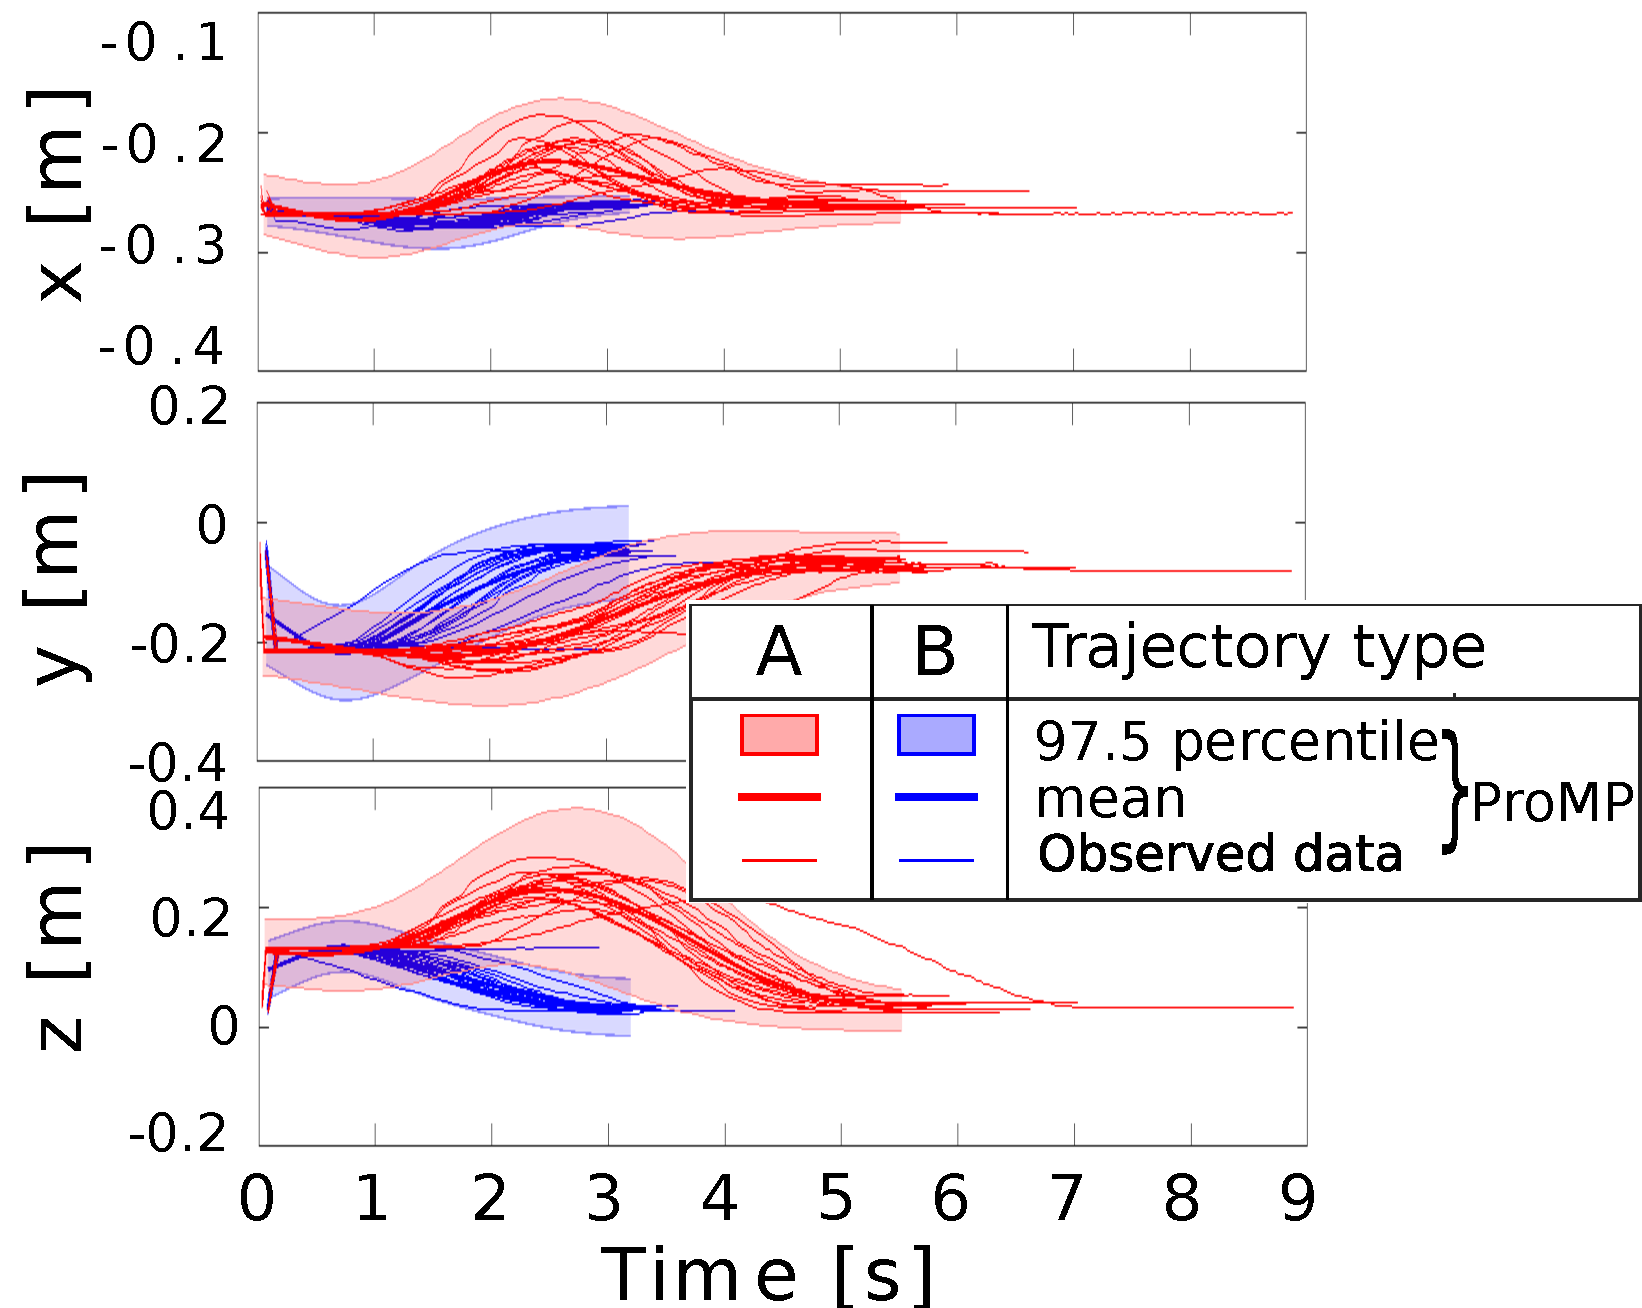
\includegraphics[height=3.8cm]{figures/positionV2.pdf}}
  \subfloat[End-effector orientation.]{\label{fig:distrib-b}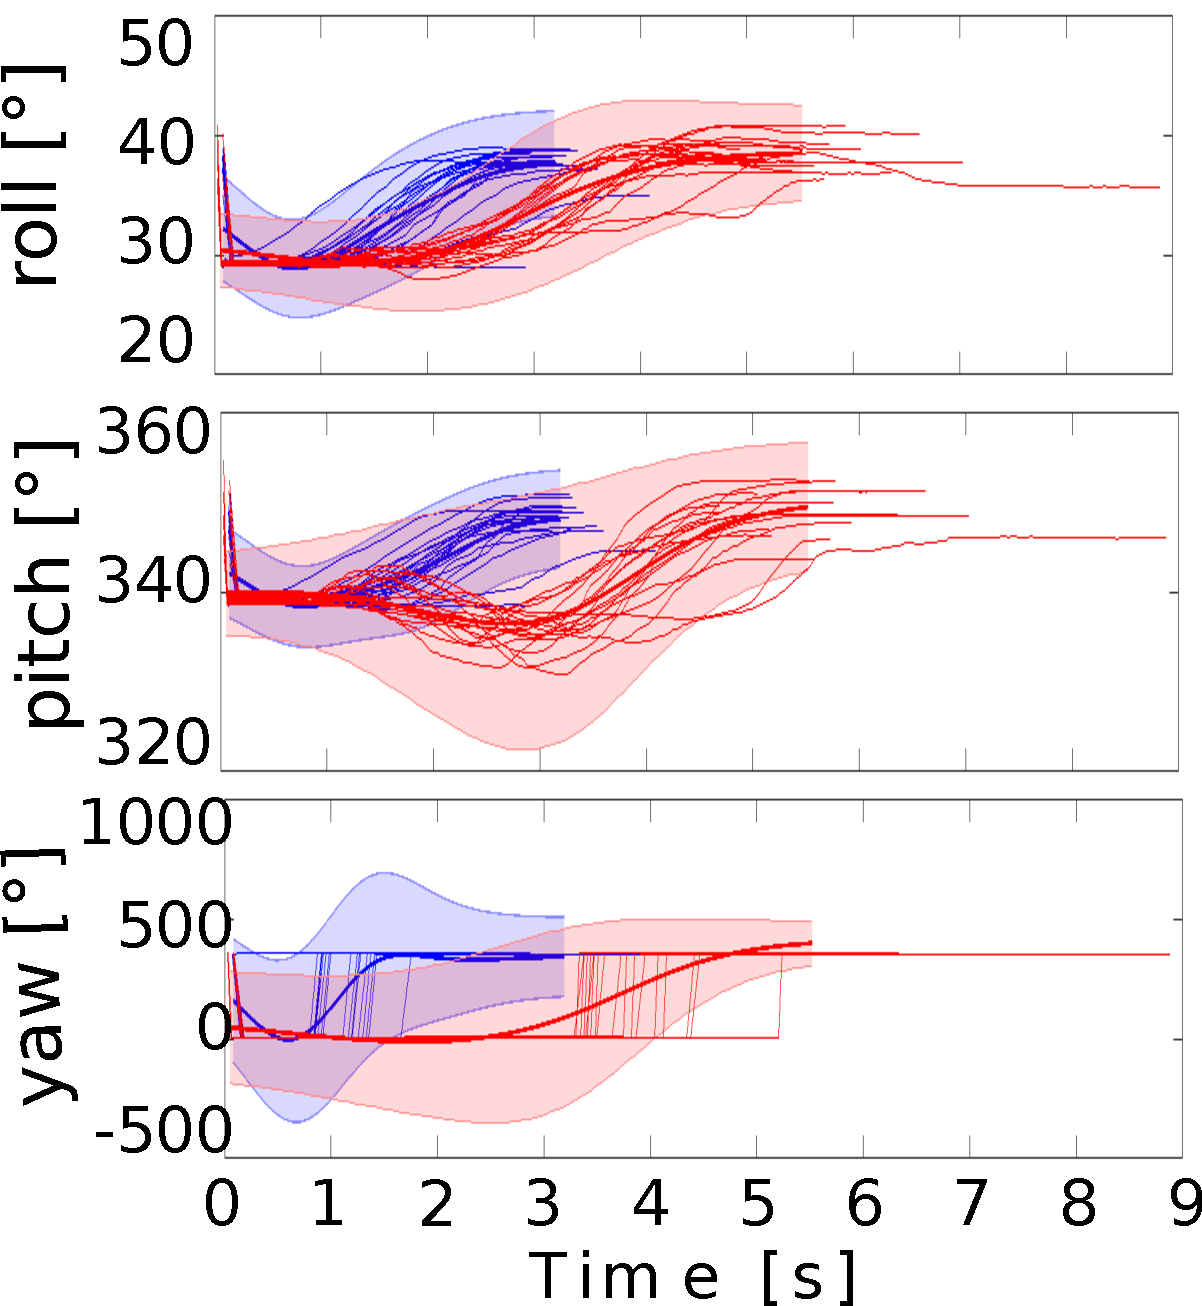
\includegraphics[height=3.8cm]{figures/orientationV2.pdf}}
 % \subfloat[Wrench norms]{\label{fig:distrib-c}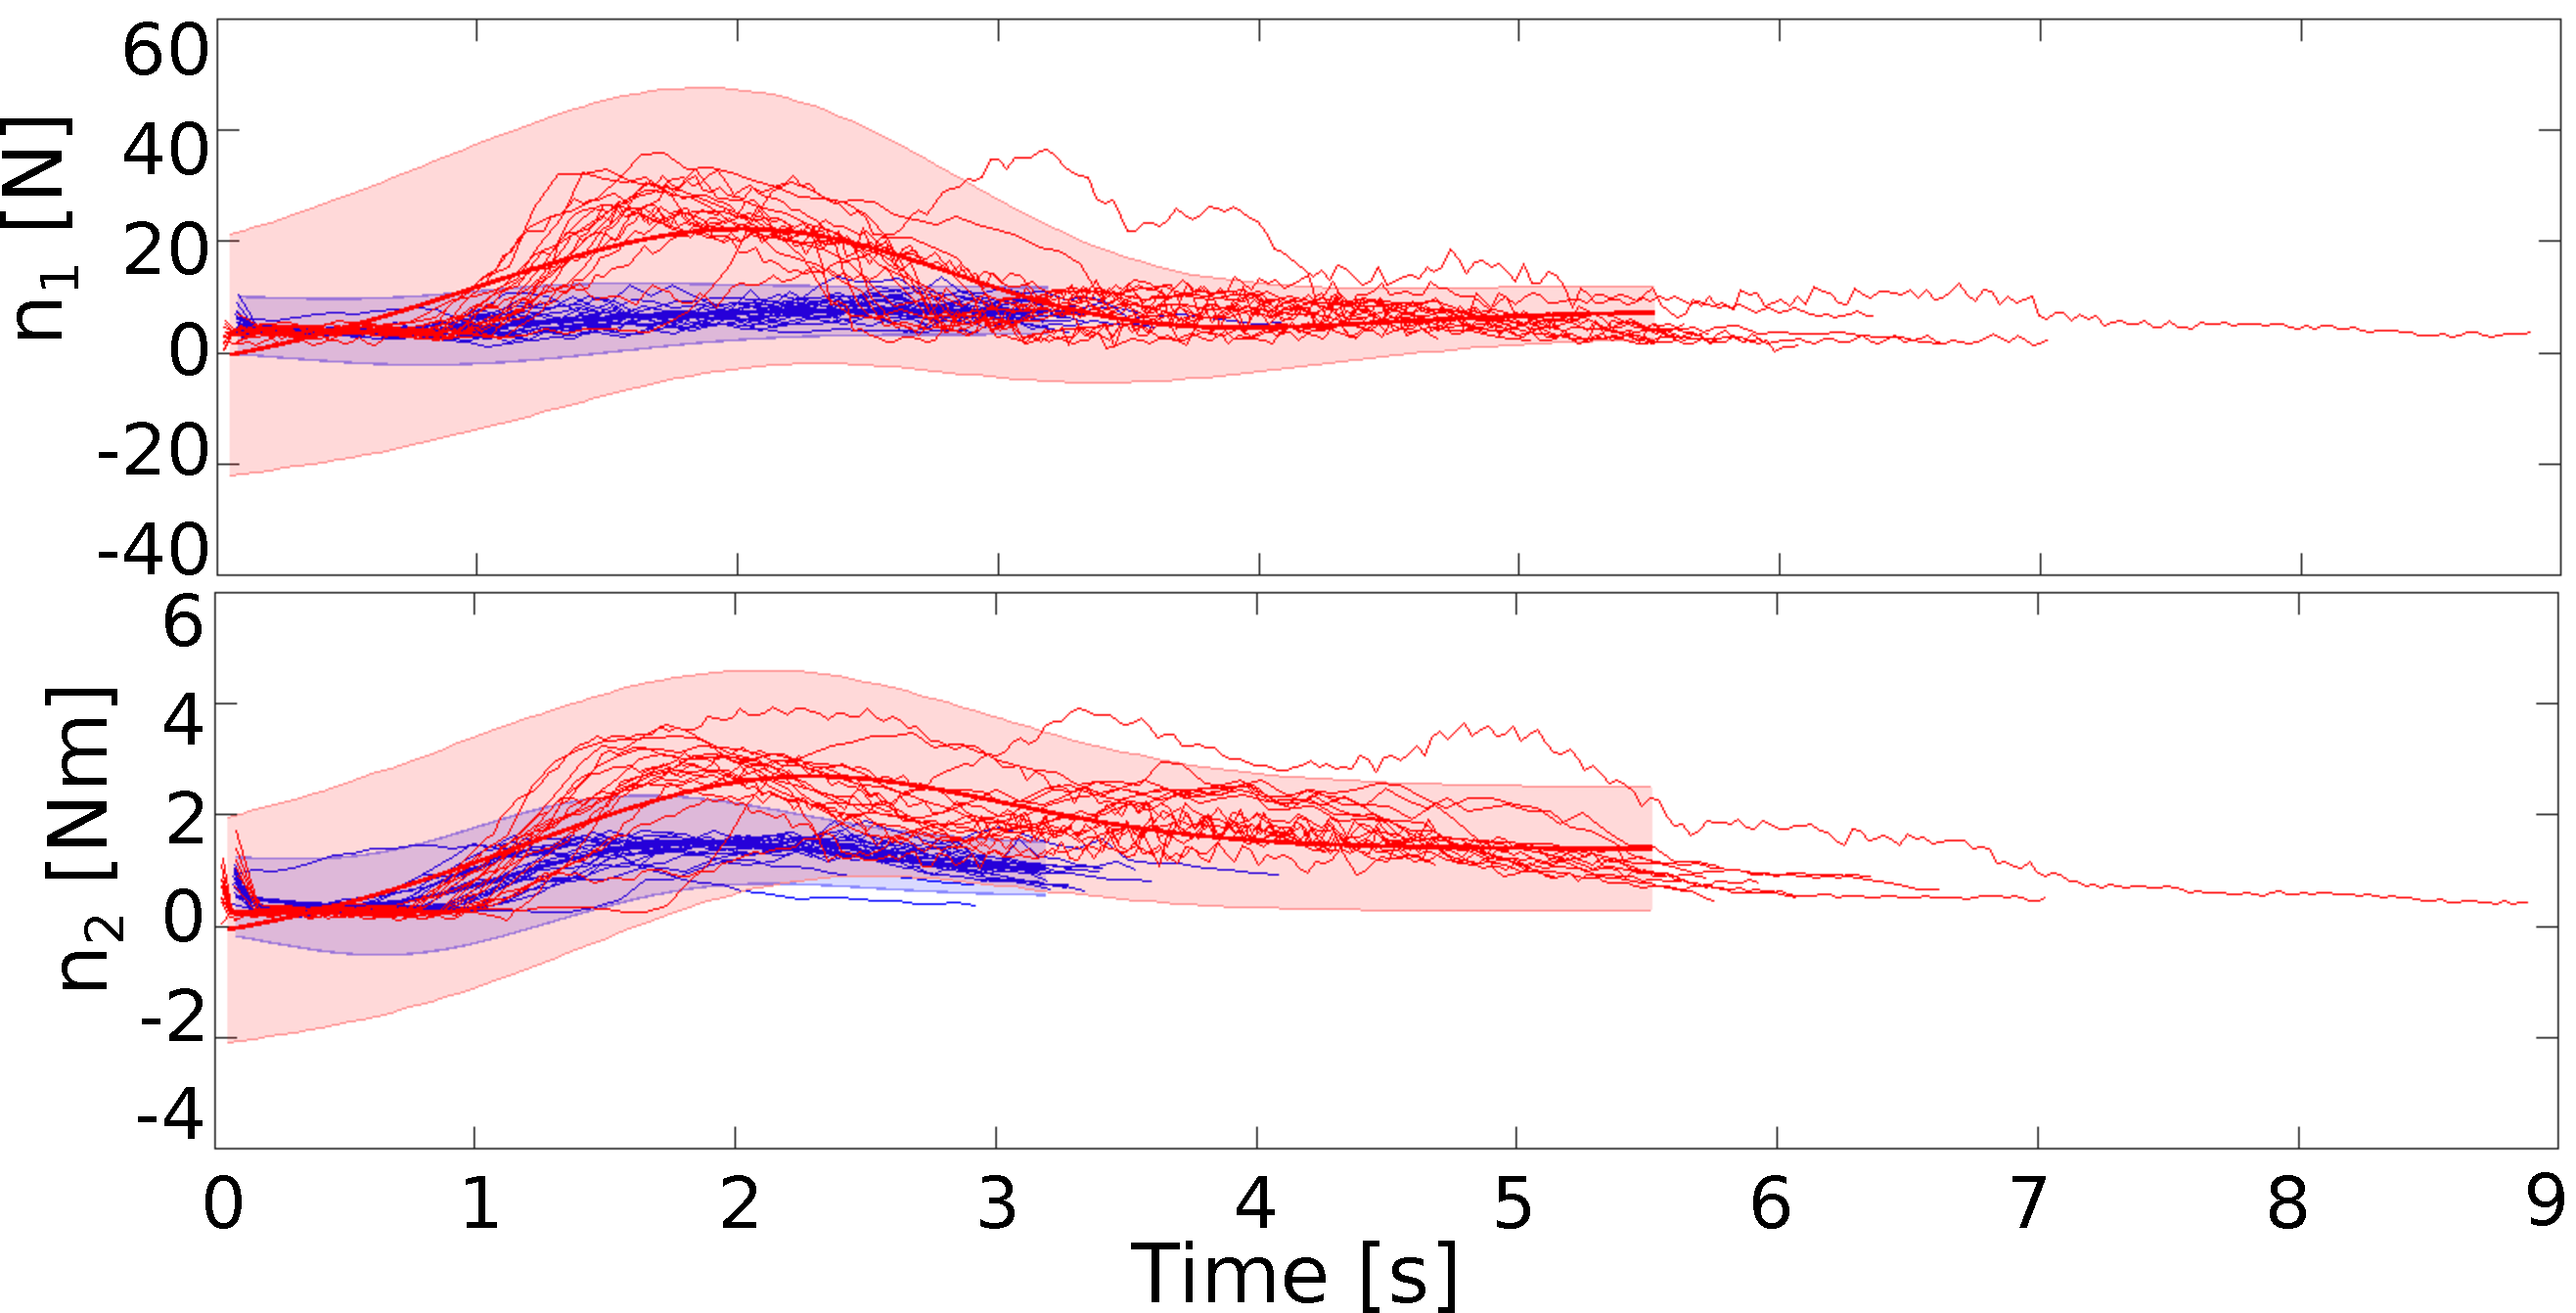
\includegraphics[width=4cm]{figures/norm.pdf}}
  \subfloat[Head orientation.]{\label{fig:distrib-d}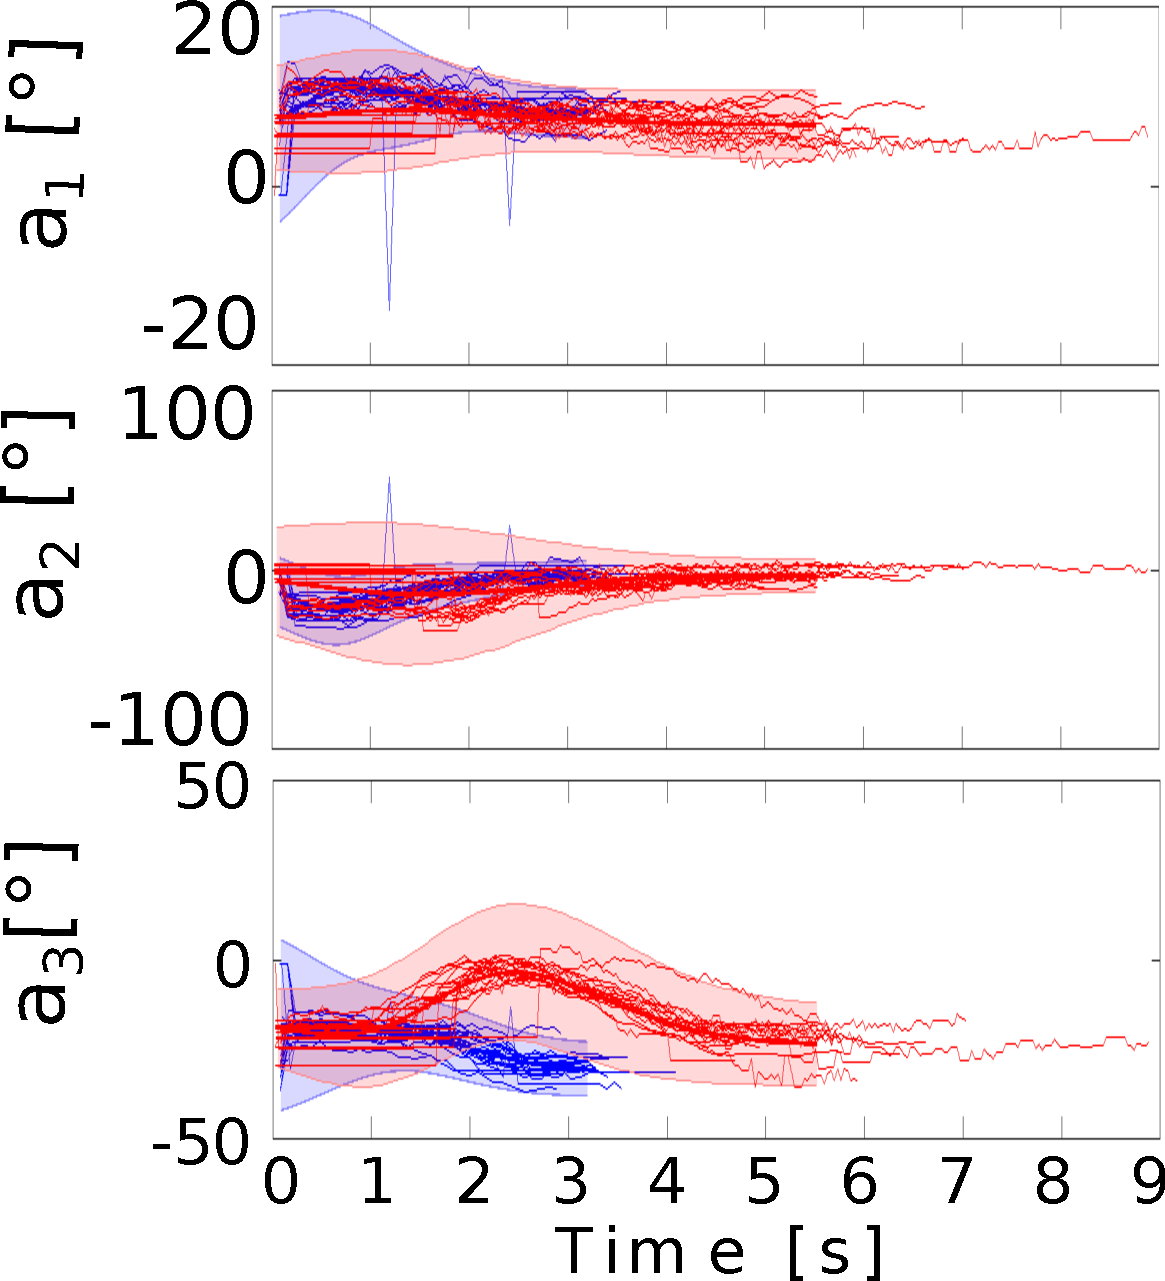
\includegraphics[height=3.8cm]{figures/headV2.pdf}}
  \caption{Demonstrations (trajectories) and primitives. In red (ProMP A) the ``curved" trajectory, and in blue (ProMP B) the ``direct" trajectory.}
  \label{fig:distrib}
\end{figure}

We taught the robot two multi-modal movement primitives that make it drop an object inside a target bin (roughly at the same position) but following two different type of trajectories coupled with the corresponding trajectories of the human partner. 
These primitives contain the Cartesian position and orientation
%, and wrenches information 
of the robot's left hand (guided by the robot operator), and the head orientation of the human partner that visually guides the robot:  $\xi(t) = [X(t), A(t)]^\top$, with $X(t) \in \Re^6$ the Cartesian pose
%, $F(t) \in \Re^2$ the wrench norms 
and $A(t)$ the roll-pitch-yaw orientation angles of the partner's head. 

We performed $20$ trajectory demonstrations per primitive action.
Fig.~\ref{fig:distrib} shows the demonstrations and the learned-distribution for the two ProMPs. 
%This figure represents the x-y-z axis of the Cartesian position (a) and the orientation (b) of the robot's left arm, the norm of the wrenches (c) measured on the arm, and the partner's head orientation (d).
%Figure~\ref{fig:distribPhy} represents the demonstration of the physical learning, with in blue the trajectory to grasp the ``octopus", and in red the trajectory to grasp the ``bottle"
%Note that the position trajectories are s because objects are placed on the same position, and that orientations and moments change because the grasping is different for the two objects.
%     \begin{figure}
%     \centering
% \subfloat[Position]{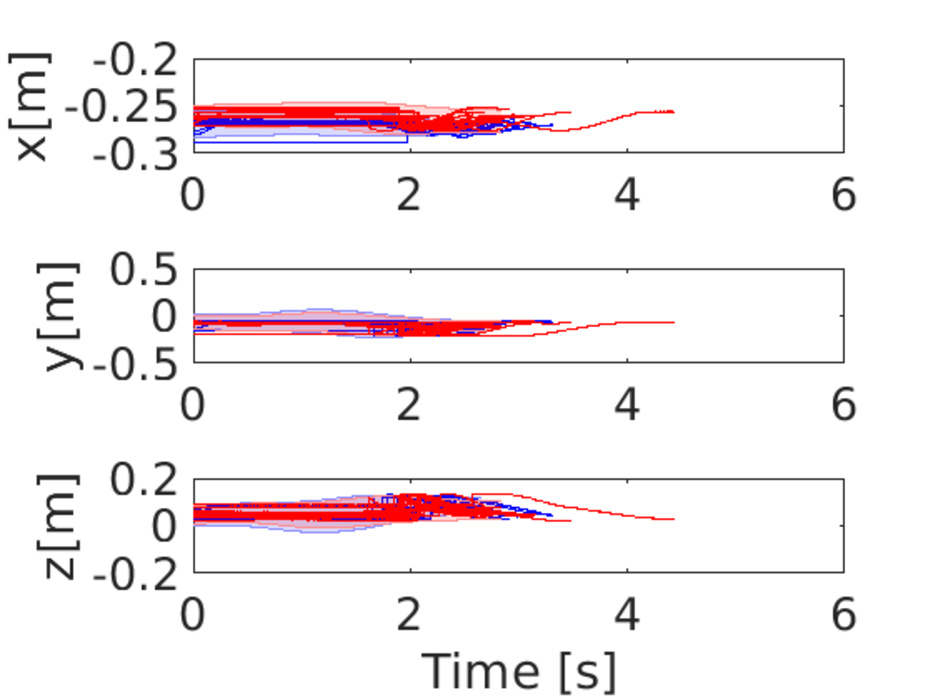
\includegraphics[width=5cm]{figures/distribPositionPhy.pdf}}
% \subfloat[Orientation]{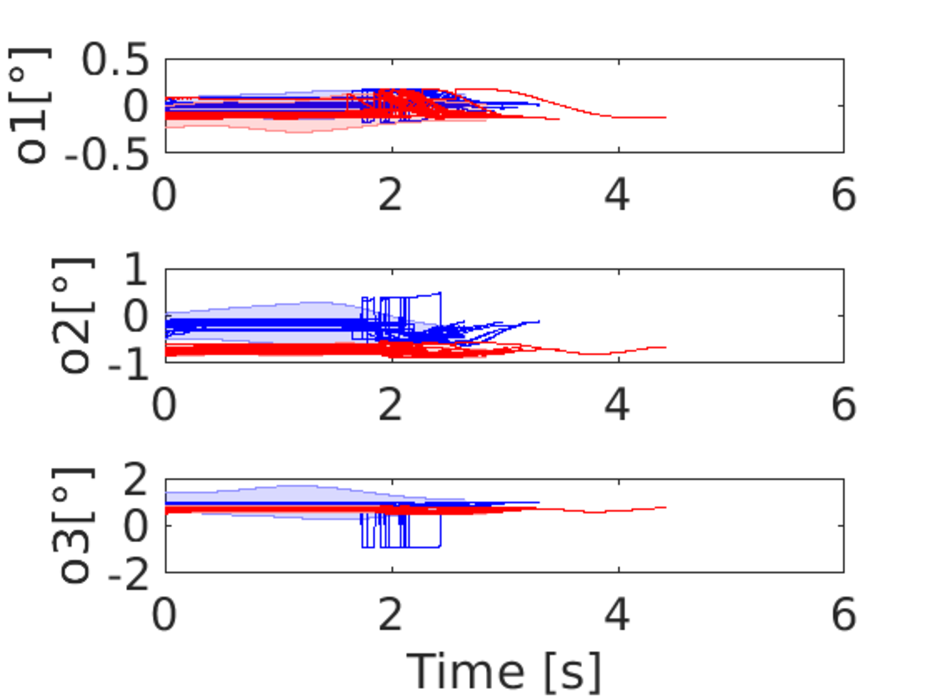
\includegraphics[width=5cm]{figures/distribOrientationPhy.pdf}}
%  \subfloat[Wrenches]{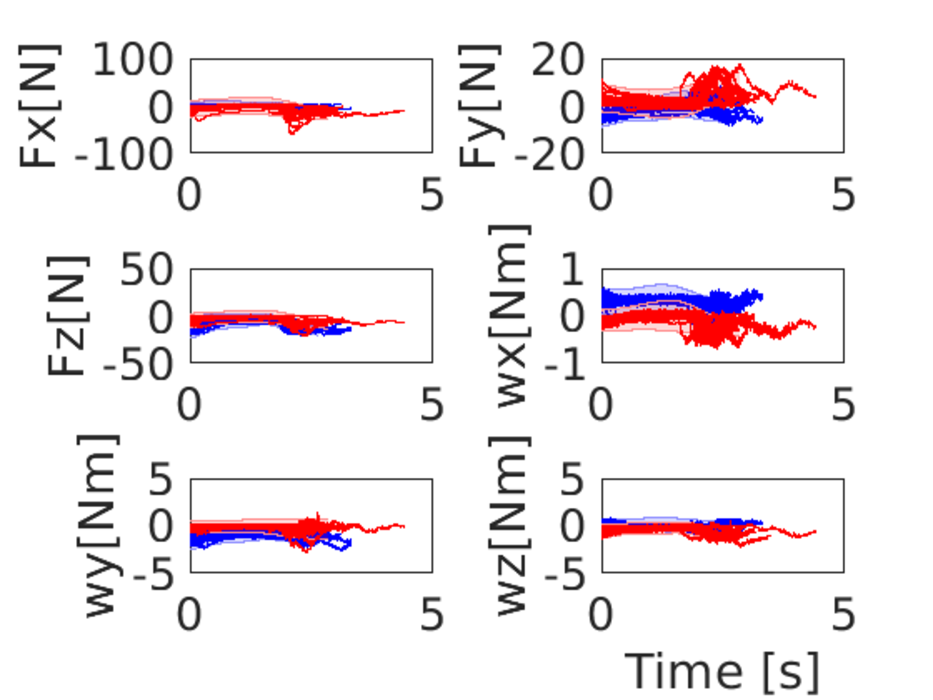
\includegraphics[width=5cm]{figures/distribWrenchesPhy.pdf}}
%\caption{The primitives computed to grasp objects.}
%  \label{fig:distribPhy}
%\end{figure}

\subsection{Activating Primitives With Gaze}
%Once the ProMPs have been learned, 

%\begin{figure}[h]
%  \centering
%      \subfloat[Example of position inference from 50\% of the head orientation trajectory.]{\label{fig:infgaze}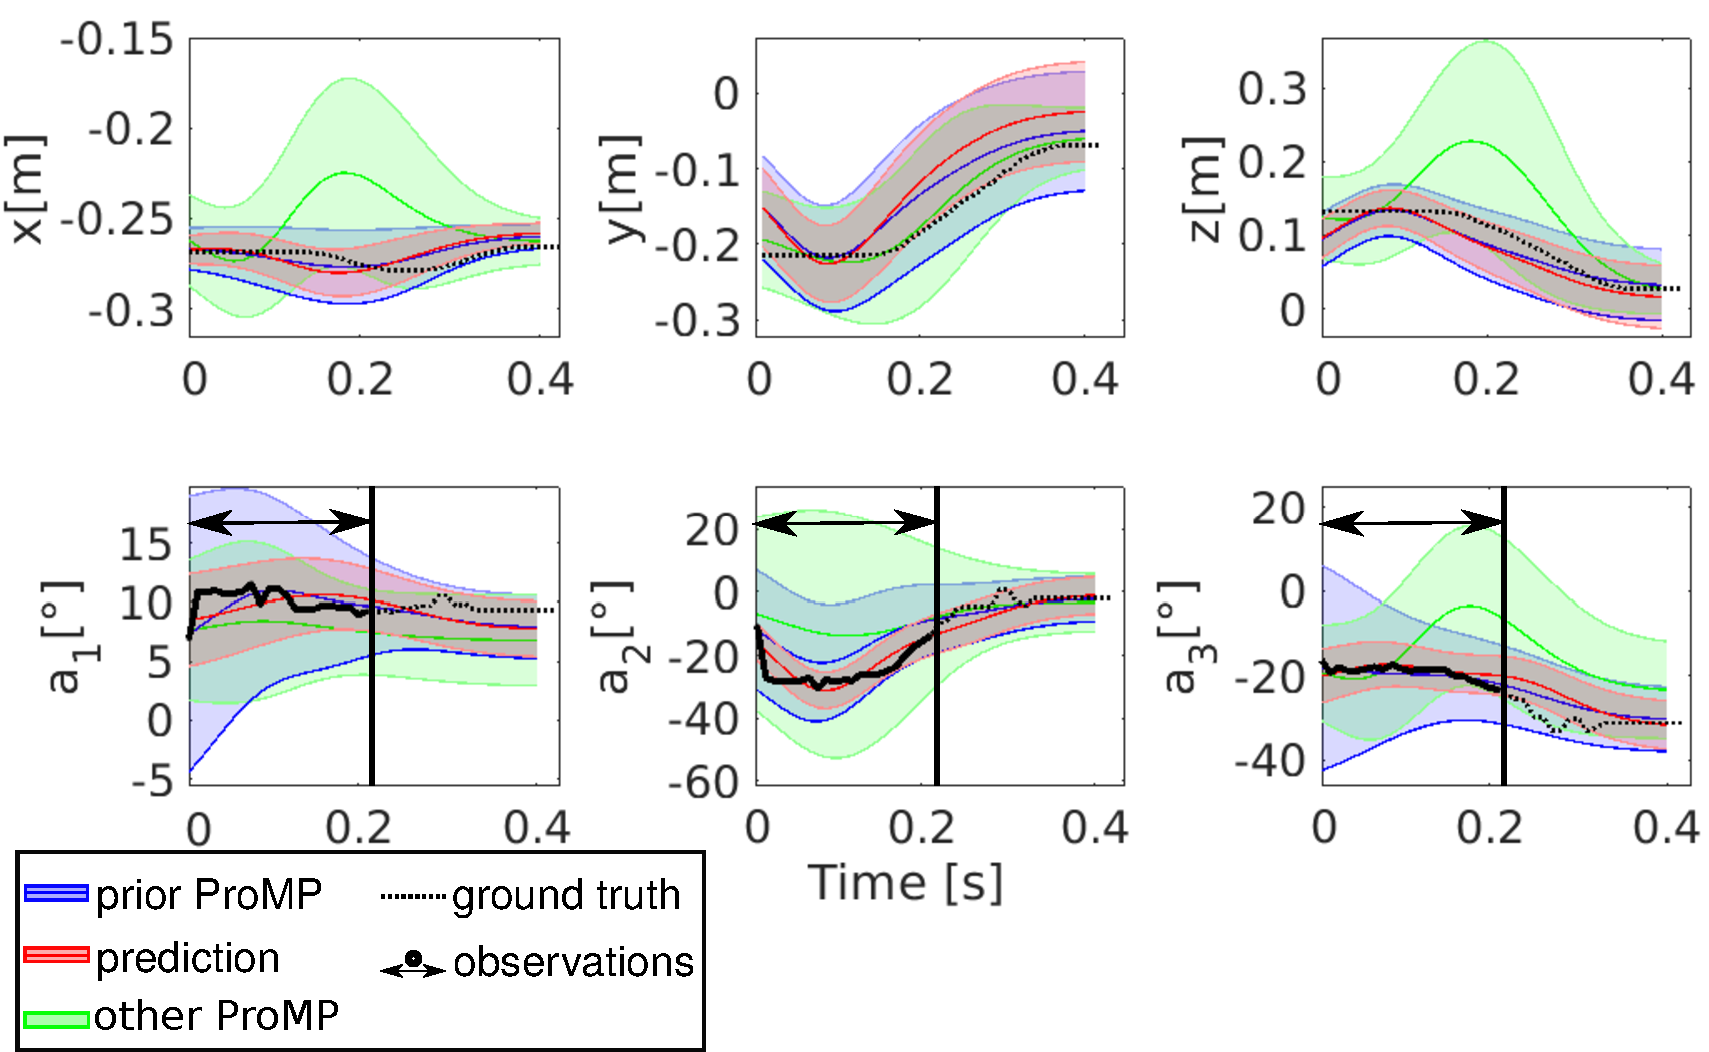
\includegraphics[width=10cm]{figures/visuInf.pdf}}%inferenceHead.pdf}}
%      \hspace{1pt}      
%    \subfloat[Number of prediction errors.]{\label{fig:predErrorgaze}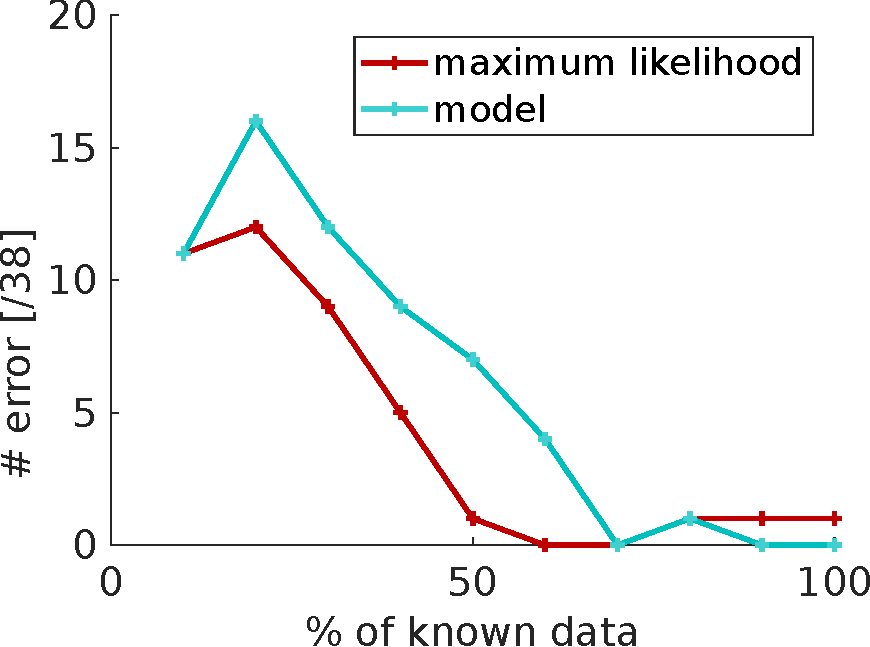
\includegraphics[width=4.5cm]{figures/visu_nbErr.pdf}}
%    \subfloat[RNMSE difference between the prior and posterior distribution.]{\label{fig:NMRSE_gaze}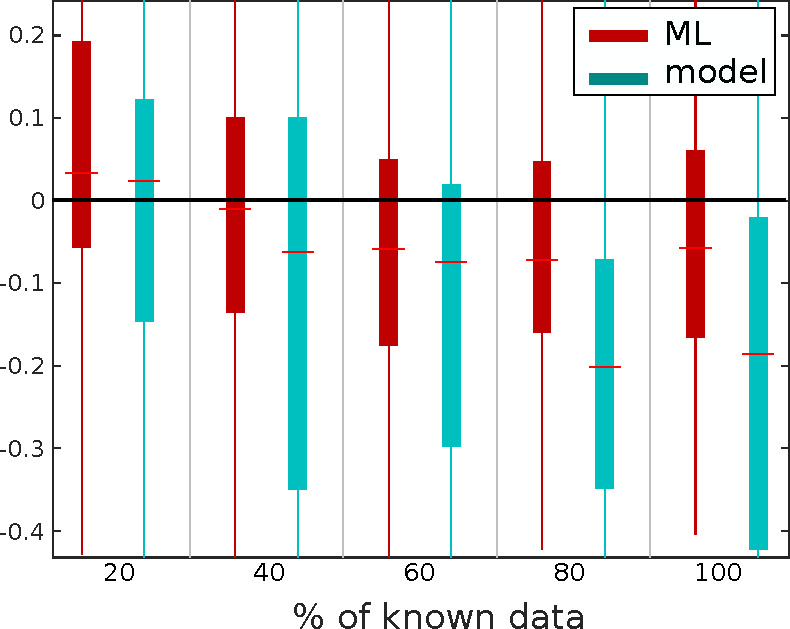
\includegraphics[width=5.5cm]{figures/visu_NRMSEDiff.pdf}}\\
%  \subfloat[Inference error of the cartesian position: average$ |X_{des} - \hat{X}|$.]{\label{fig:errInfgaze}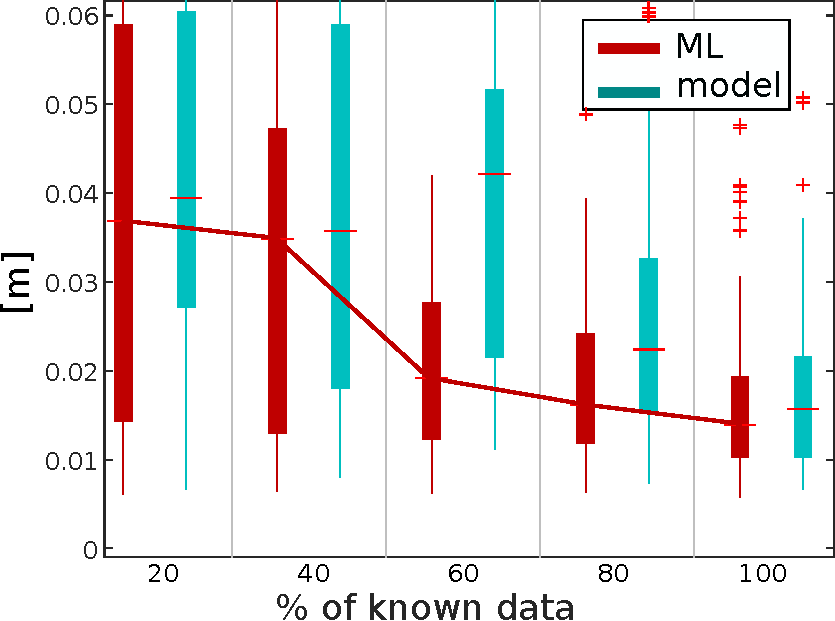
\includegraphics[width=6cm]{figures/visu_ErrInf.pdf}}
%    %errorPriorVSinfV3
%\caption{Prediction error from gaze.}
%  \label{fig:gazeResult}
%\end{figure}
%

\begin{figure}
  \centering
%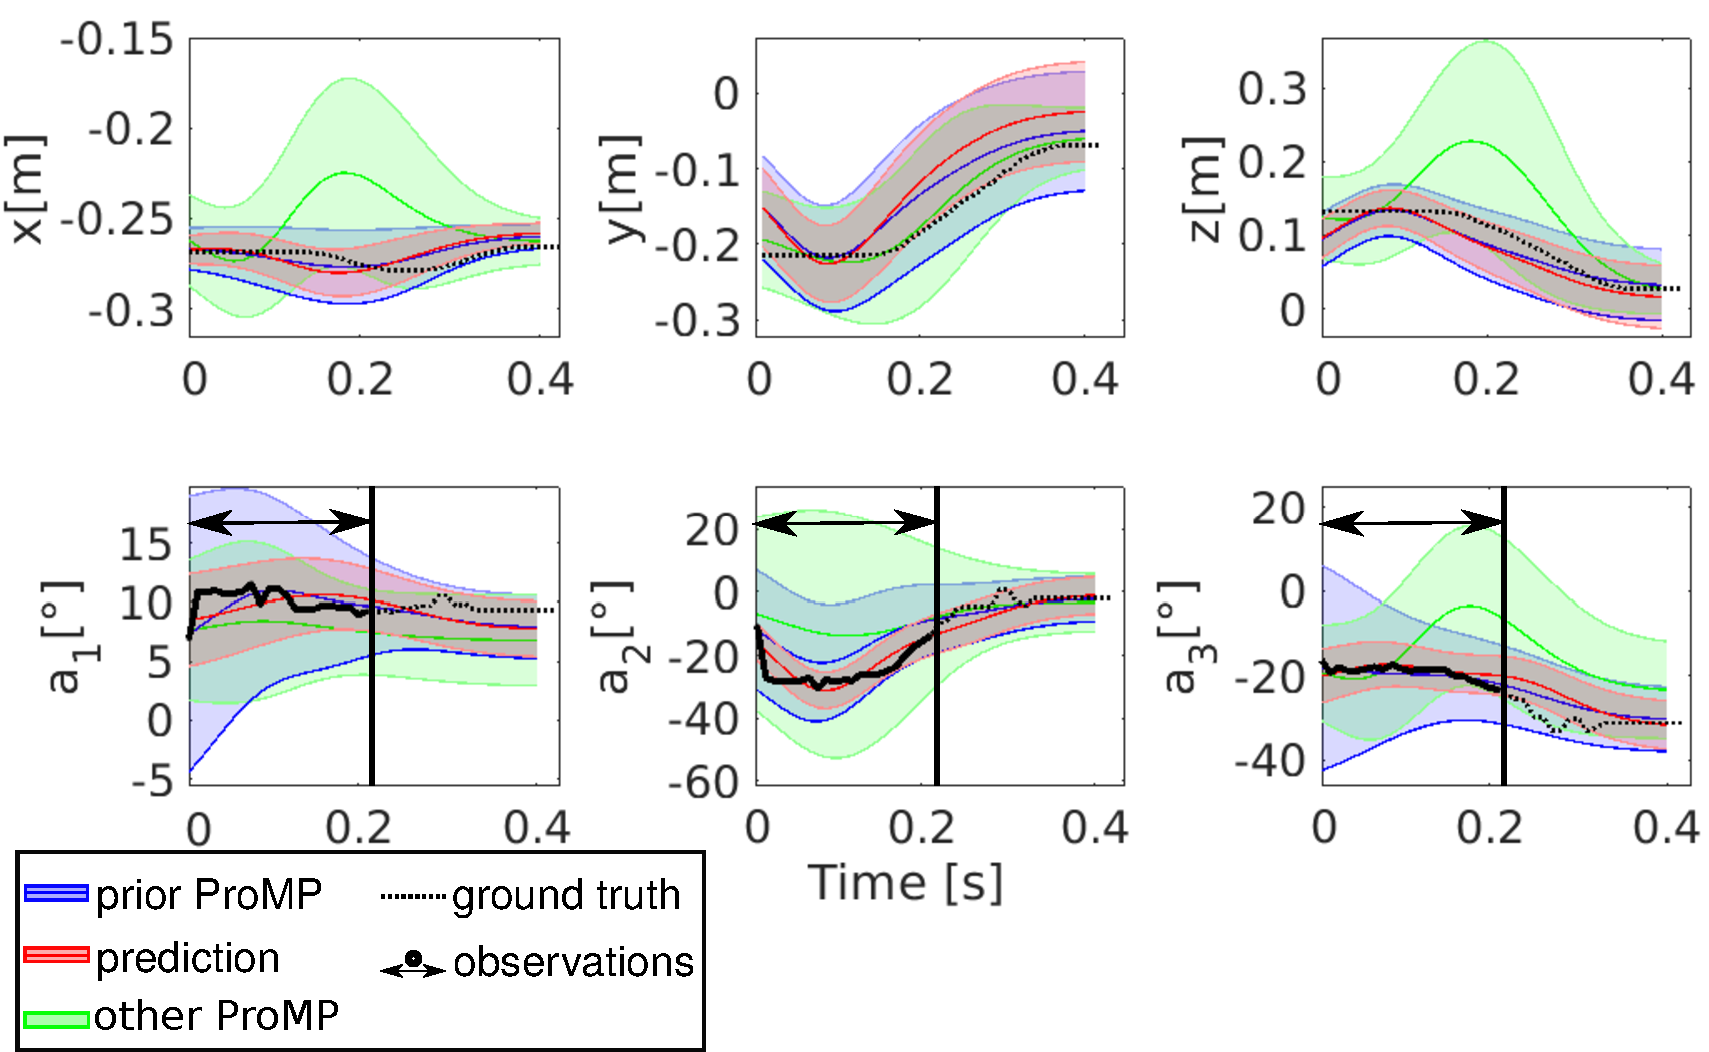
\includegraphics[width=\hsize]{figures/visuInf.pdf}\\%inferenceHead.pdf}}
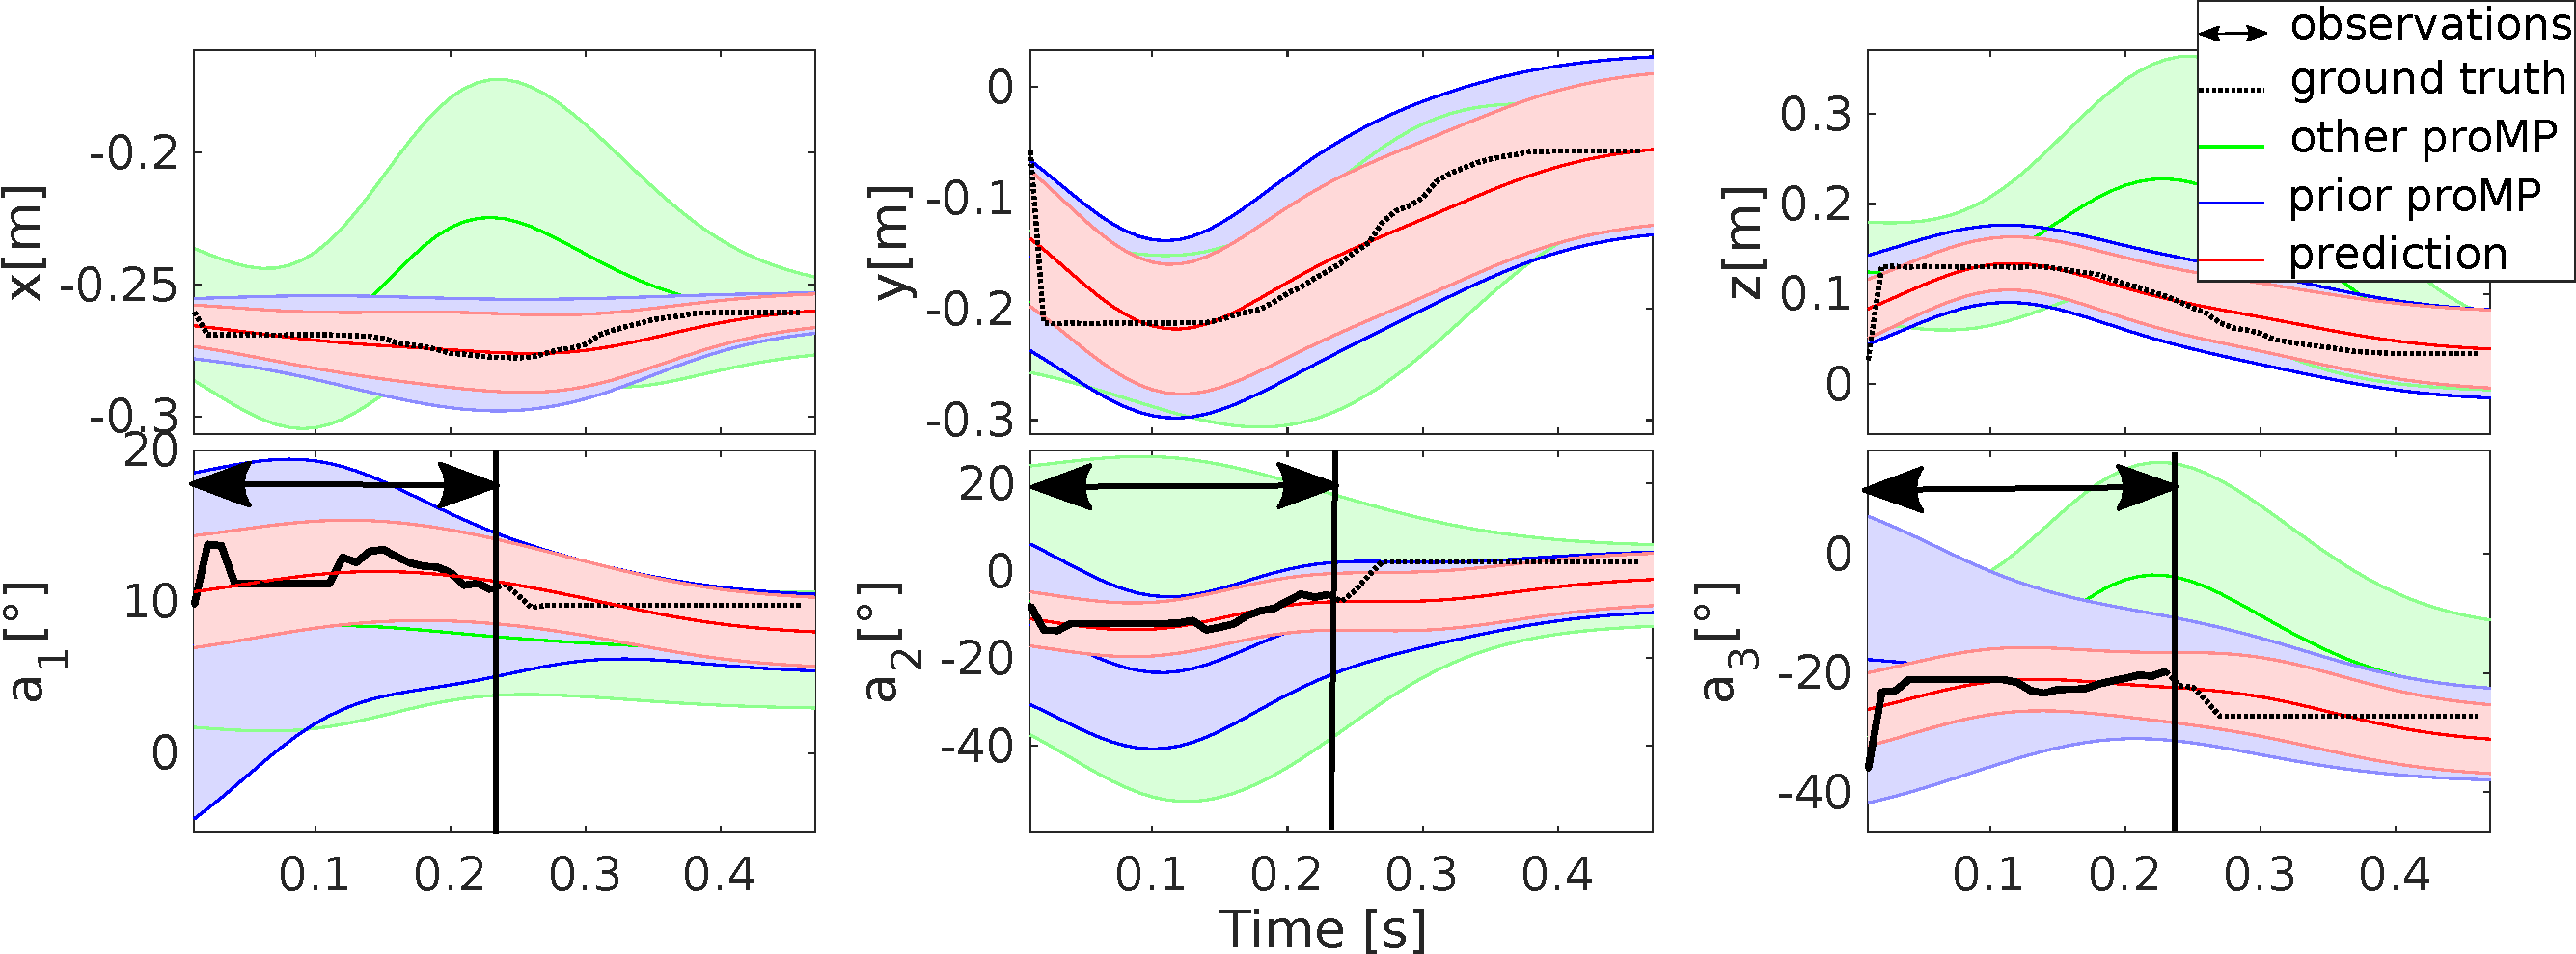
\includegraphics[width=\hsize]{figures/visionN.pdf}%inferenceHead.pdf}}

\caption{Example of position inference from 50\% of the head orientation trajectory.\label{fig:infgaze} The dots represent the trajectory the robot has to perform (ground truth). The black curves represent the measurements done by the robot. The blue distribution represents the recognized ProMP and the green distribution the other ProMP. The red distribution represents the posterior of the blue distribution, computed from the measured data.}
\end{figure} 

The gaze cue is used to identify the current action. This procedure has two advantages. First, it does not require physical interaction, which could ease interacting with the robot for some people. Second, it enables to improve the prediction of intended trajectory, especially in case of ambiguous primitives that overlap and could make it difficult to obtain a good prediction with few early observations. An intuitive case is shown in Fig.~\ref{fig:intuition}.

\begin{wrapfigure}{r}{0.5\textwidth} 
\hspace{2pt}
\vspace{-40pt}
  \begin{center}
    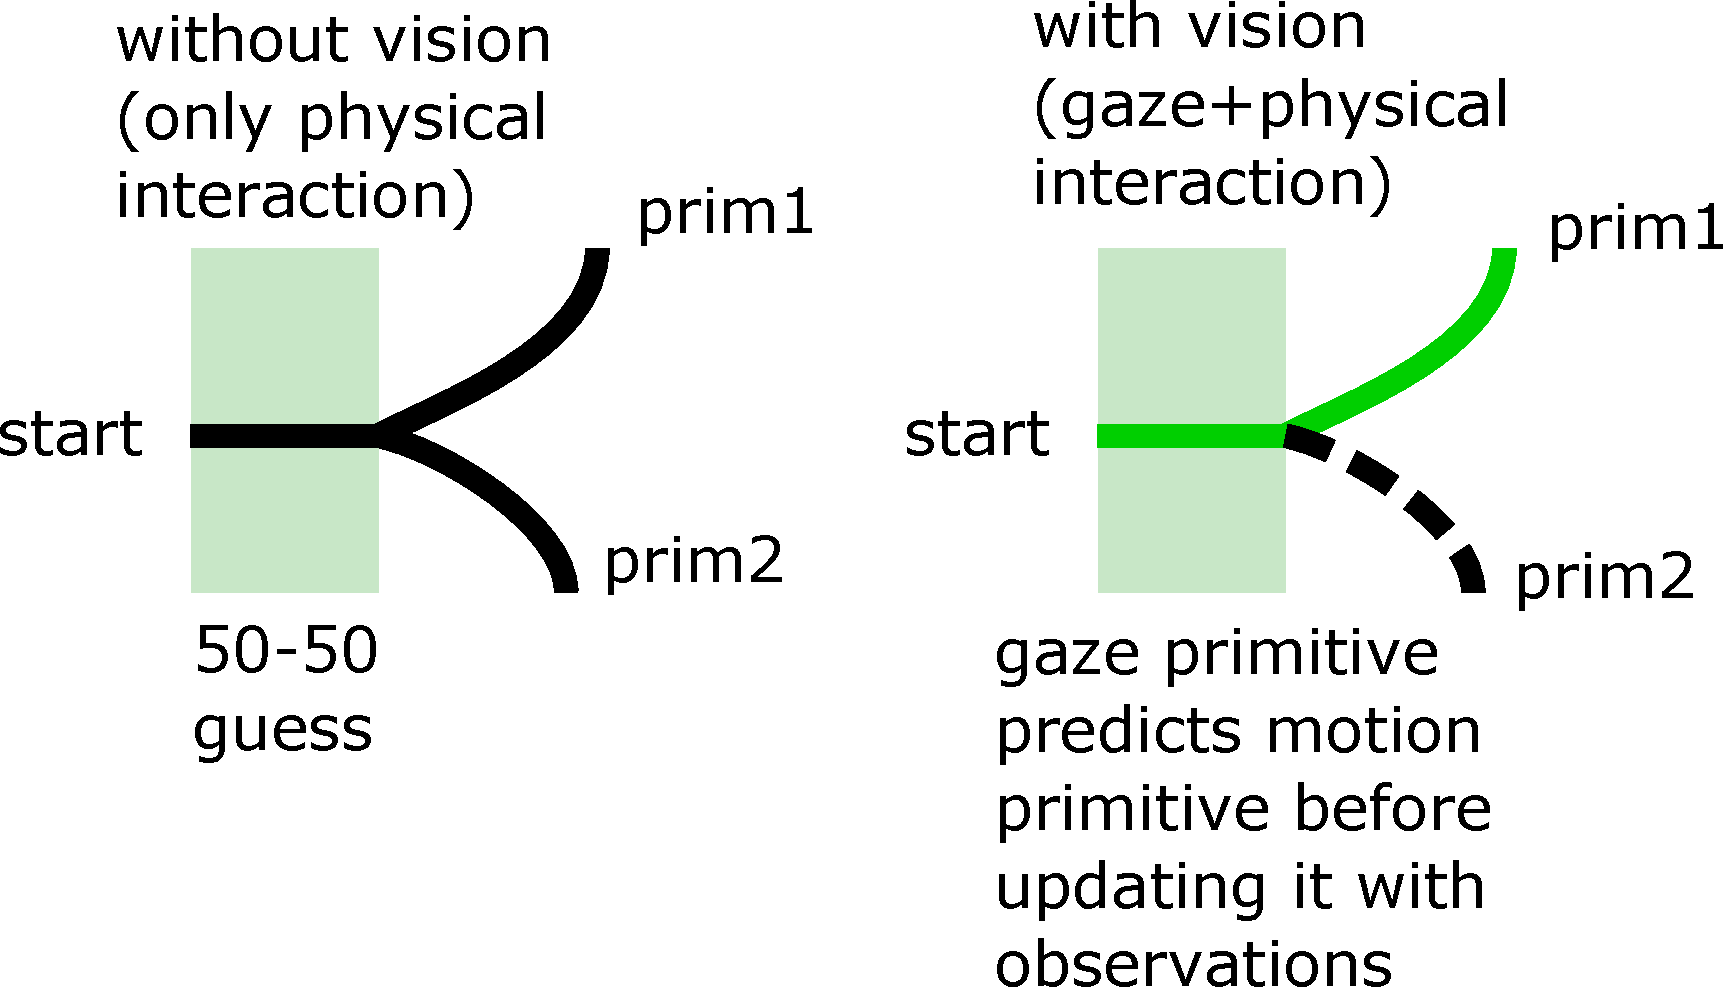
\includegraphics[width=0.5\textwidth]{figures/intuition.pdf}%{./Pictures/mainscreen1.png}
    \caption{Gaze helps disambiguate two overlapping primitives.}
    \label{fig:intuition}
  \end{center}
  \vspace{-30pt}
\end{wrapfigure} 

From~\cite{oriane2017}, we retain two methods to compute the time modulation: ``maximum likelihood'' (\textit{ML}) and ``\textit{model}'', where the latter consists on estimating the trajectory duration according to the global partner's head orientation variation:
% presented in our previous paper (\cite{oriane2017} Sec.~3.4). We adapt the ``model'' for the visual modality with: 
``$\delta_{n_o} = A(n_o) - A(1)$''.

We tested off-line the gaze prediction of the trajectories on the acquired data set using cross-validation.
Fig.~\ref{fig:infgaze} shows a prediction example after having observed $50$\% of the trajectory. The inferred trajectory is the mean trajectory of the red posterior distribution. Note that this posterior distribution is included in the prior distribution and pass by the observed data with some \textit{flexibility}, that correspond to the expected measurement noise fixed a-priori.
%For the sake of clarity, this figure does not show the orientation of the robot's arm. %\sout{The trajectory in black represents the ``ground truth", that is the real trajectory the robot has to perform. In black points, the trajectory observations from which the inference is done. In blue, we represent the most likely ProMP that corresponds to the observations (here the ProMP "B" that is the ``direct" trajectory), in green the second one. Finally in red, the posterior ProMP B (\textit{i.e.} after having updated the prior ProMP in blue to by-pass by the observation). }
%An apriori fixed variable in the posterior distribution computation corresponds to the noise estimation of the observation. Due to this
%Thanks to a fixed-variable that represents the measurement noise, the posterior distribution pass approximatively by the observation (instead of roughly). 
Even though the partner's head orientation observations are not accurate, the prediction is good enough to allow the robot to complete the task correctly.

%We performed $38$ different trials using each computational method presented in~\ref{ssec:prediction}. 
Fig.~\ref{fig:predErrorgaze} represents the error of ProMP recognition according to the percentage of observations of the test trajectory. 
%The average duration of a trajectory is about $89.6$ samples, with an average interval of $6.67e^{-2}$ seconds between samples. 
The longer the head trajectory is observed, the smaller is the prediction error, for both methods for computing the time modulation. 
%However, when the last percents of the trajectories are known, some errors of recognition reappear because since trajectories end positions are identical, the last measurements don't help the recognition, and because the orientation of the partner's head orientation is retrieved from the Intraface program that is not able to detect the partner's head orientation when the user looks too much downward (\textit{e.g.}, the end of the trajectory).
This figure also shows that the \textit{model} is less accurate than the \textit{ML} method when the robot observes less than $70\%$ of the whole trajectory, while with more observation the \textit{model} method is a slightly more accurate. Since head movements are fast, the robot can use the whole head movement trajectory and still react quickly. So, we can use the \textit{model} method to allow the robot to recognize which ProMP to follow for the visual guidance. With $70$\% observation of a trajectory, there is no ProMP type recognition error, thus, the robot can roughly infer the trajectory to perform (which corresponds to $~3$ seconds).   

We represent in Fig.~\ref{fig:errInfgaze} the average error of the Cartesian position of the inferred trajectory. It shows that the error of the predicted trajectory goes from $4cm$ ($10\%$ of the trajectory) to $2$cm (from $80\%$). Thus, the more the robot observes its partner's head trajectory, the more it is able to achieve it own movement intended by its partner.
%If we look back at Fig.~\ref{fig:infgaze},

However, we can wonder if the posterior distribution is more accurate than the prior. It would be the case if the partner's head orientation was totally correlated to the robot's hand position and the measurement accurate enough to infer exactly the end-trajectory. Fig.~\ref{fig:NMRSE_gaze} represents the difference of the Normalized Root Mean Square Error (NRMSE) between the prior and the posterior distribution. From $40\%$ of the trajectory observation, this difference is inferior to zero, meaning that by updating the distribution, the robot improves the trajectory inference. Thus, the visual guidance can be used to determine which ProMP the robot has to follow, but also to adapt the ProMP distribution from the user's head guidance in an accurate way.

To achieve a better accuracy, we assume the physical interaction will more indicated. To verify this assumption, the next session presents the physical guidance experiment.

\begin{figure}
  \centering    
    \subfloat[Number of prediction errors.]{\label{fig:predErrorgaze}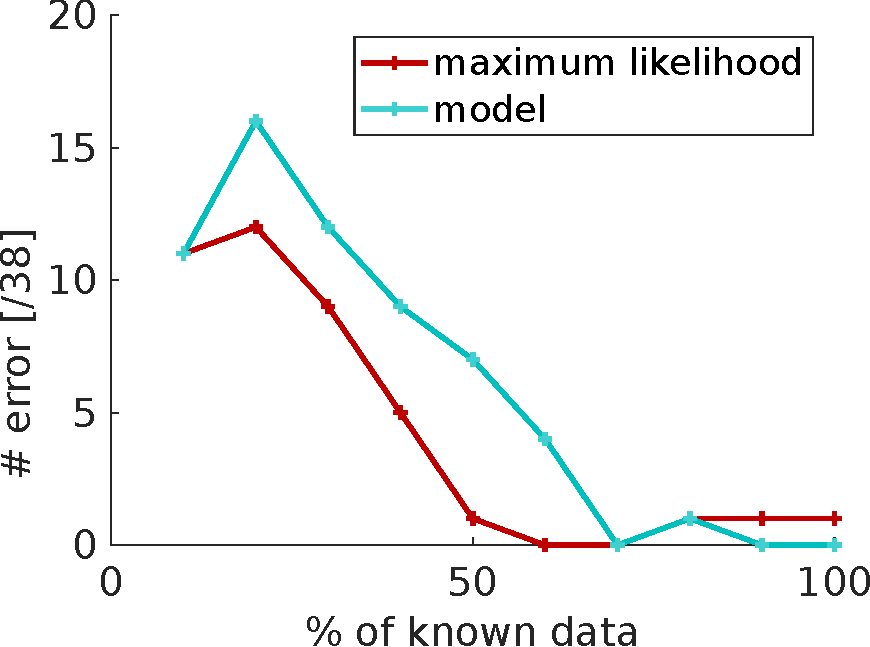
\includegraphics[width=173.5 pt]{figures/visu_nbErr.pdf}}
  \subfloat[Inference error of the Cartesian position: average$ |X_{des} - \hat{X}|$.]{\label{fig:errInfgaze}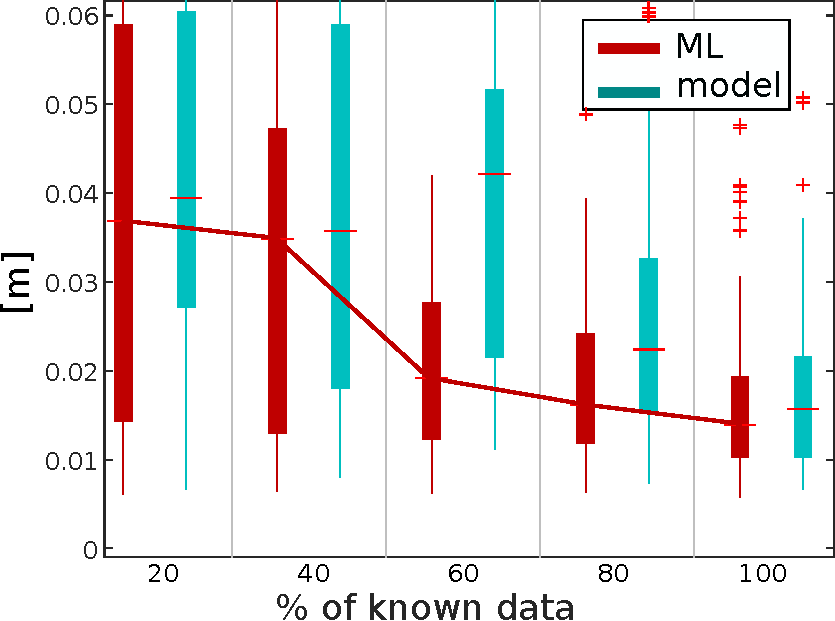
\includegraphics[width=173.5 pt]{figures/visu_ErrInf.pdf}}\\
    \subfloat[RNMSE difference between the prior and posterior distribution.]{\label{fig:NMRSE_gaze}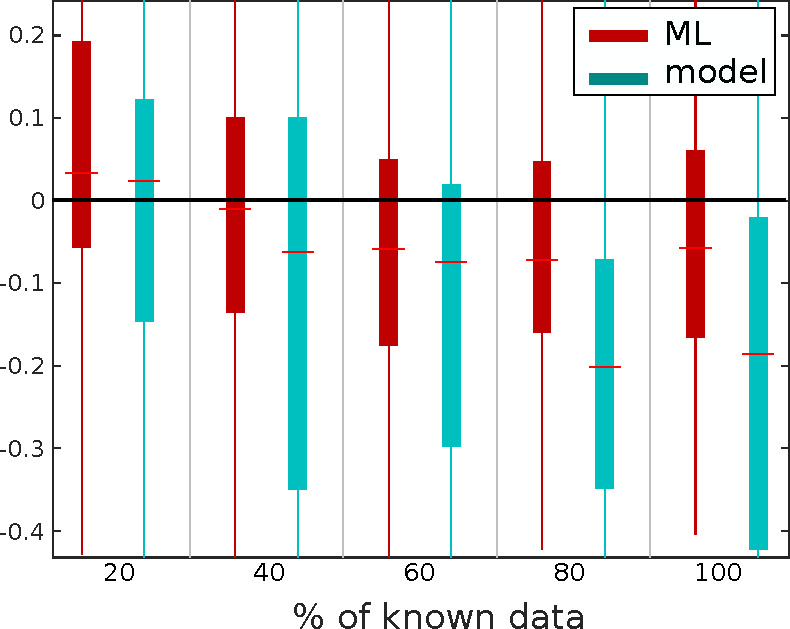
\includegraphics[width=173.5 pt]{figures/visu_NRMSEDiff.pdf}}
\caption{Visual guidance analysis.}
  \label{fig:gazeResult}
\end{figure}


%\begin{figure}
%\centering
%
\includegraphics[width=0.5\hsize]{figures/todo.pdf}
%\caption{\todo{the primitives activated by gaze}}
%\label{fig:activations}
%\end{figure}
%\begin{table}
%\caption{\todo{Prediction error (RMSE) for activating the ProMP with gaze}}
%\label{table:errors}
%\end{table}
\subsection{Inference of Intended Trajectories With Physical Guidance}
%\begin{figure}
%  \centering
%  \subfloat[Example of trajectory inference from physical guidance.]{\label{fig:physInf}
%    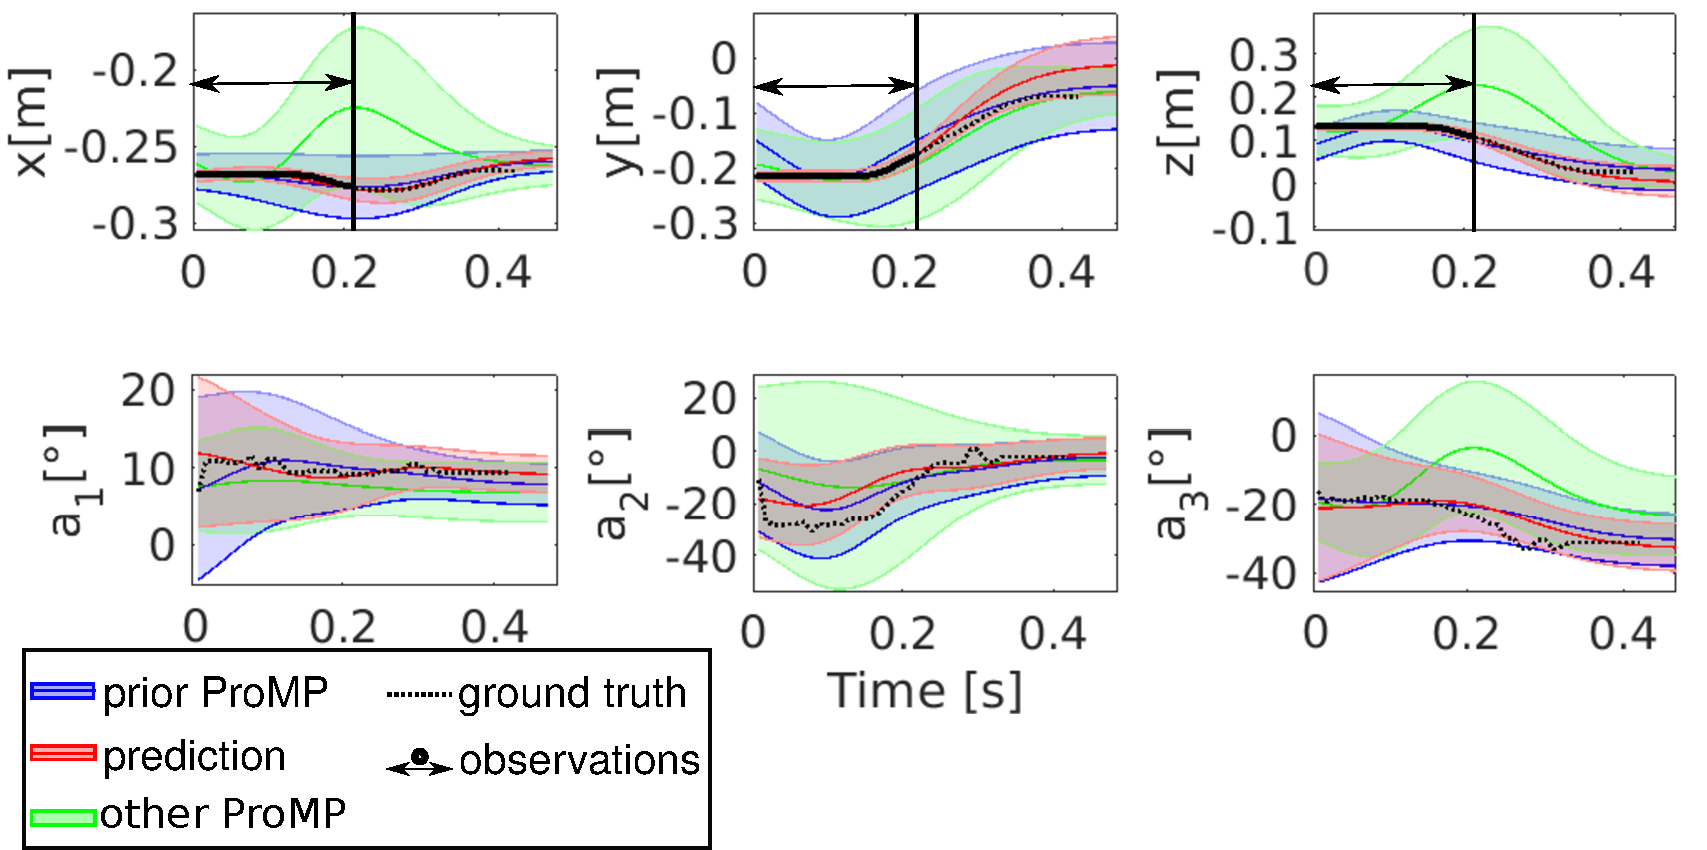
\includegraphics[width=\hsize]{figures/positionInf.pdf}}
%    %inferencePhyDrop.pdf}}
%          \hspace{1pt}      
%  \subfloat[Inference error of the cartesian position: average$ |X_{des} - \hat{X}|$.]{\label{fig:infErrPhy}\includegraphics[width=5.8cm]{figures/%yErrorBoxPlotPhyDrop.pdf}}
%  positionInfErr.pdf}}
% \subfloat[average $|nrmse_{post}-nrmse_{prior}|$.]{\label{fig:RNMSE-phy-b}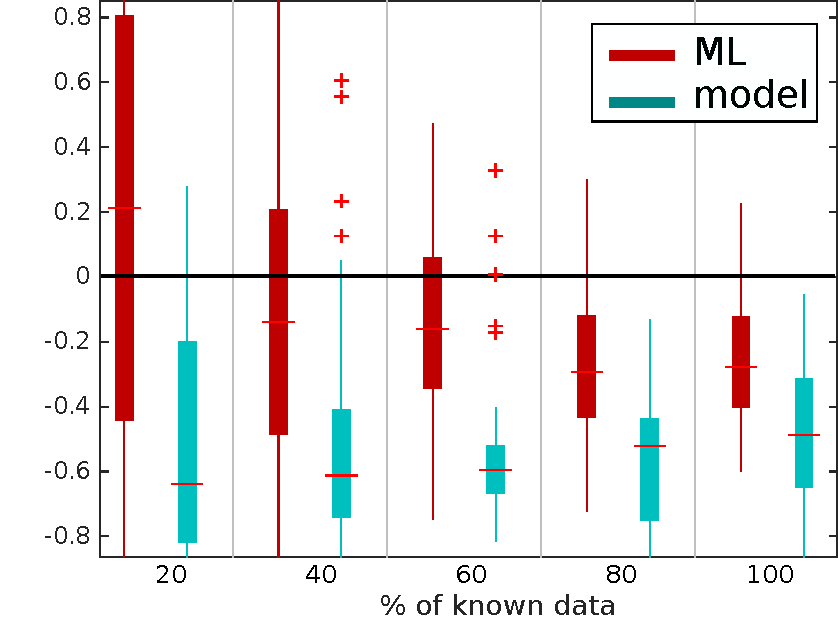
\includegraphics[width=5.2cm]{figures/positionNMRSDiff.pdf}}
% \caption{Inference errors with physical guidance.}
%\label{fig:physicalPred}
%\end{figure}
\begin{figure}
  \centering
        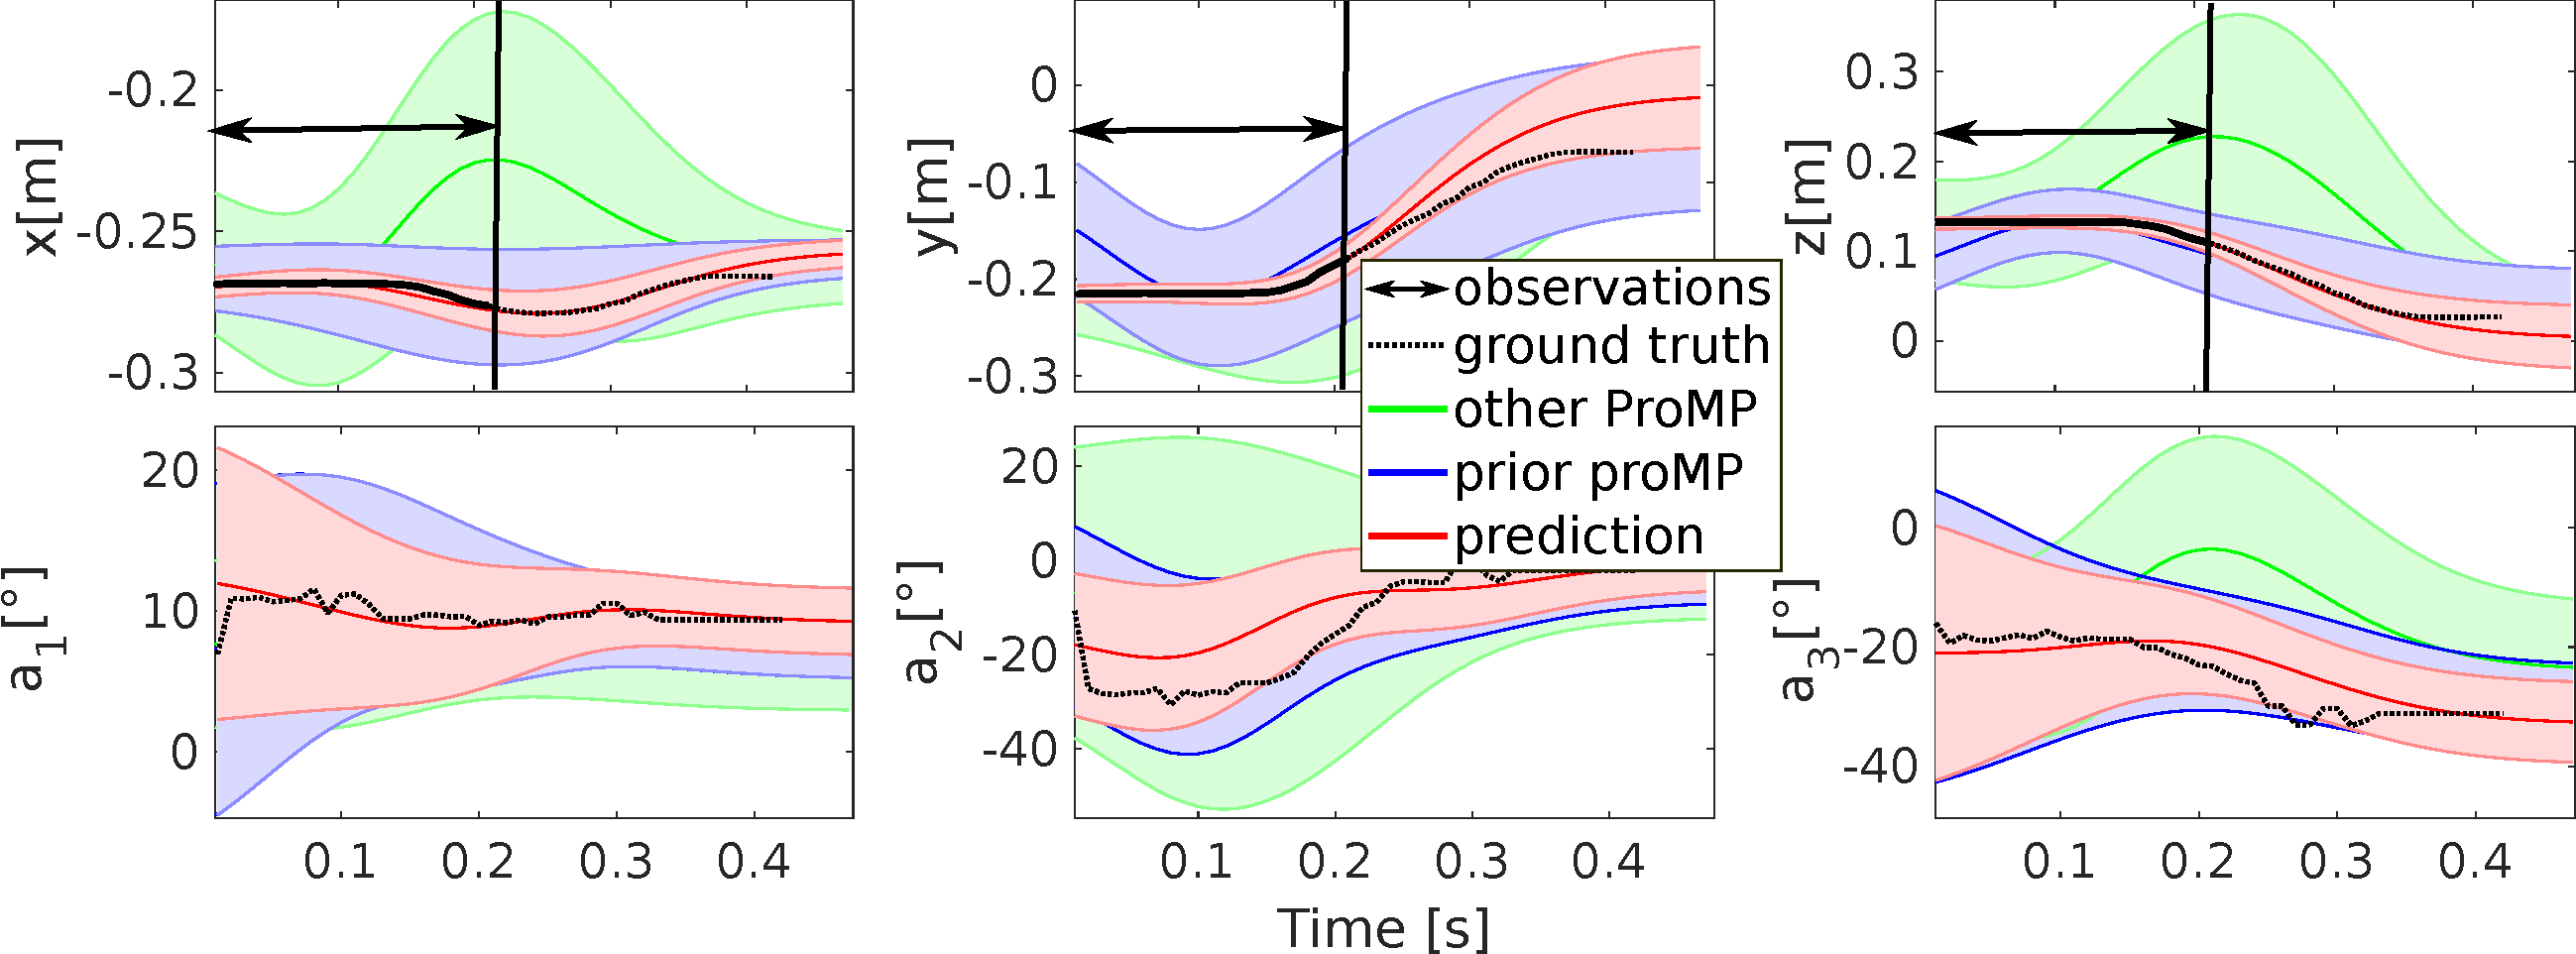
\includegraphics[width=\hsize]{figures/positionN.pdf}
      \caption{Example of trajectory inference from physical guidance.\label{fig:physInf}}
\end{figure}

\begin{figure}
  \centering     
  \subfloat[Inference error of the Cartesian position: average$ |X_{des} - \hat{X}|$.]{\label{fig:infErrPhy}\includegraphics[width=173.5 pt]{figures/%yErrorBoxPlotPhyDrop.pdf}}
  positionInfErr.pdf}}
 \subfloat[average $|nrmse_{post}-nrmse_{prior}|$.]{\label{fig:RNMSE-phy-b}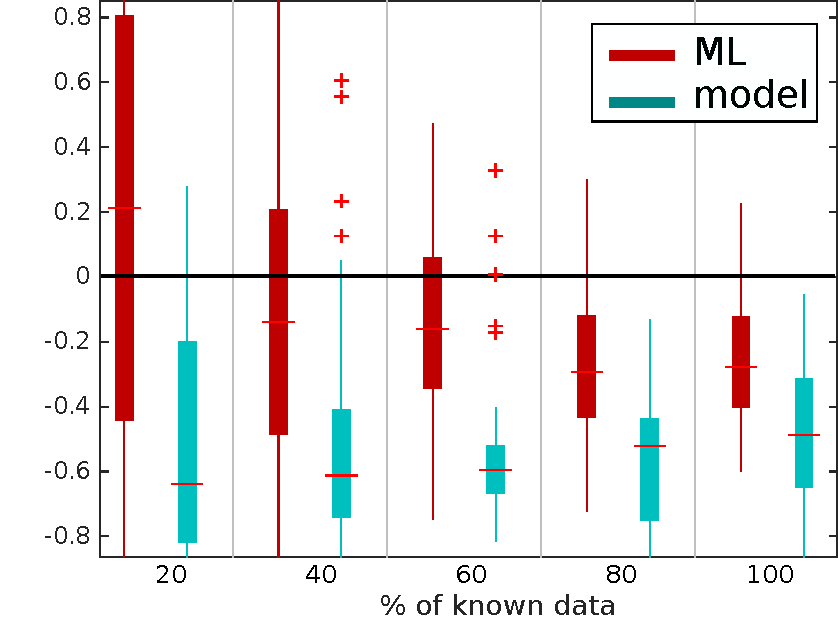
\includegraphics[width=173.5 pt]{figures/positionNMRSDiff.pdf}}
% NMRSDpriorVSpostPhyDrop
 \caption{Physical guidance analysis.}
\label{fig:physicalPred}
\end{figure}

The same prediction experiment from early-demonstrations than the previous section is presented here with haptic signals. Fig.~\ref{fig:physInf} presents an example of such prediction. If we compare to the visual experiment, we can note that the inferred trajectory (mean of the red posterior distribution) is closer to the ground truth. 
%We have done $20$ different trials. 
%and results are presented at Figure~\ref{fig:physicalPred}.
%Each time, the ProMP distributions are learned using the $19$ other trajectories. We perform these tests for each computational method presented in~\ref{ssec:prediction}.
%Figure~\ref{fig:alpha_physic} shows that the time modulation parameter is best estimated using the Maximum Likelihood method and that using the mean method, this time modulation is not correct enough.
Fig.~\ref{fig:infErrPhy} verifies this idea. It represents the average distance between the inferred trajectory ($\hat{X}$) and the ground truth ($X_{des}$), and the results show that the trajectory prediction using physical estimation is more accurate than the visual estimation, whether with the \textit{model} or the \textit{ML} method, with an average of less than $1cm$ of distance error for the \textit{model} and from $3cm$ ($40\%$ of known data) to $1cm$ ($80\%$) for the \textit{ML}. Moreover, Fig.~\ref{fig:RNMSE-phy-b} shows that the posterior distribution of the ProMP improves the accuracy of the trajectory, mainly for the \textit{model} method which explains why the distance error using this method is short in the previous figure. 

Now, we can wonder if using the two modalities could improve the performance of this inference ability. Thus, the next section is the multi-modal experiment on the same data set.
%\par}
%Note that the model method is more efficient than the maximum likelihood method, .
%Finally, we can see the number of recognition error in Fig.~\ref{fig:erorPhy} : this number of recognition error is important, but didn't disturb, as shown in~\ref{fig:physInfWrong}, where the inference is correct even though it is based on the wrong ProMP.
%
%\begin{figure}
%\centering
%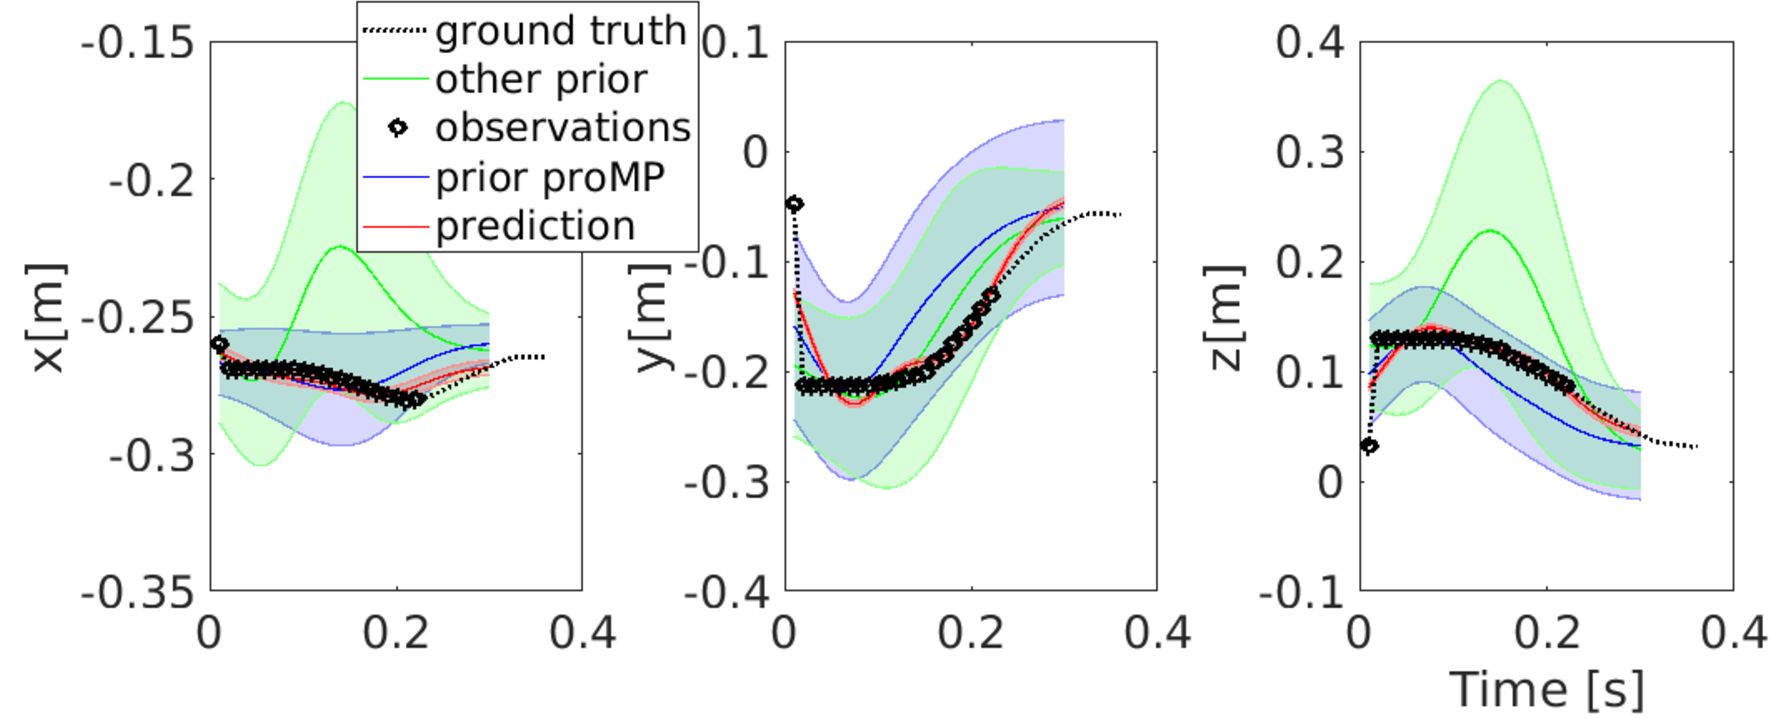
\includegraphics[width=12cm]{figures/InfwithErrorReco.pdf}
%\caption{A primitive predicted after Cartesian position observations of 50\% of a trajectory with a wrong ProMP recognition}
%\label{fig:physInfWrong}
%\end{figure}
%
%\begin{table}
%\caption{\todo{Prediction error (RMSE) }}
%\label{table:errorsPrediction}
%\end{table}
%\ori{This last figure and paragraph can be deleted}
%\ori{Finally, figure~\ref{fig:RNMSE-phy} shows that in opposite to visual recognition result, the posterior distribution improves the inference done with the prior distribution, since the NMRSD difference between the posterior with the prior is negative from $60$\% of observations.  We can note there is still few improvement because the trajectories doesn't contains a lot of variation, in opposite to our previous work in~\cite{oriane2017}. Thus, the prior distribution is already near to the expected trajectory.}
%
%\begin{figure}[htp]
%  \centering
%  \subfloat[RNMSE of the posterior distribution]{\label{fig:RNMSE-phy-a}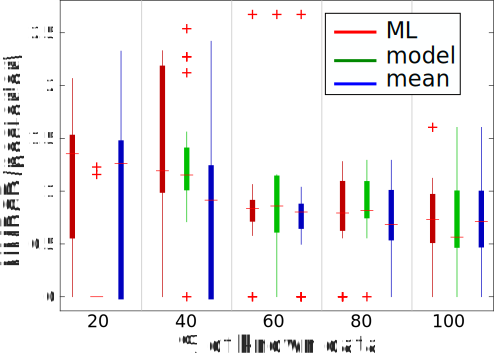
\includegraphics[width=7cm]{figures/NMRSDPhy.pdf}}
%  \subfloat[RNMSE difference between the prior and posterior distribution]{\label{fig:RNMSE-phy-b}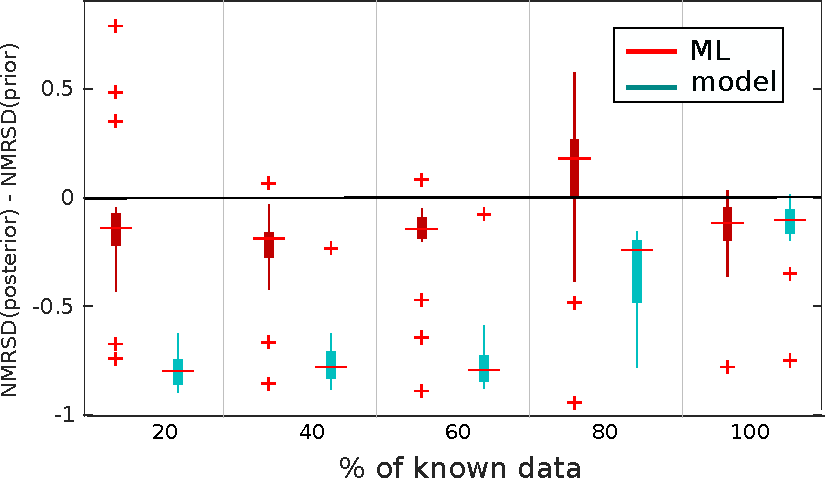
\includegraphics[width=7cm]{figures/NMRSDpriorVSpostPhy.pdf}}
%\caption{Prediction error (NRMSE) from physical guidance}
%\label{fig:RNMSE-phy}
%\end{figure}
%
%%%%%%%%%%%%%%%%%%%%%%%%%%%%%%%%%%%%%%%%%%%%%%%%%%%%%%%%%%%%%%%%%%%%%%%%%%%%%%%%%
%\section{Video}
%
%\towrite{Describe the video attachment}
%
%The video attachment shows the capabilities of our system. 
%
%%%%%%%%%%%%%%%%%%%%%%%%%%%%%%%%%%%%%%%%%%%%%%%%%%%%%%%%%%%%%%%%%%%%%%%%%%%%%%%%
\subsection{Inference of Intended Trajectories With Multi-modal guidance}
\begin{figure}
  \centering
%	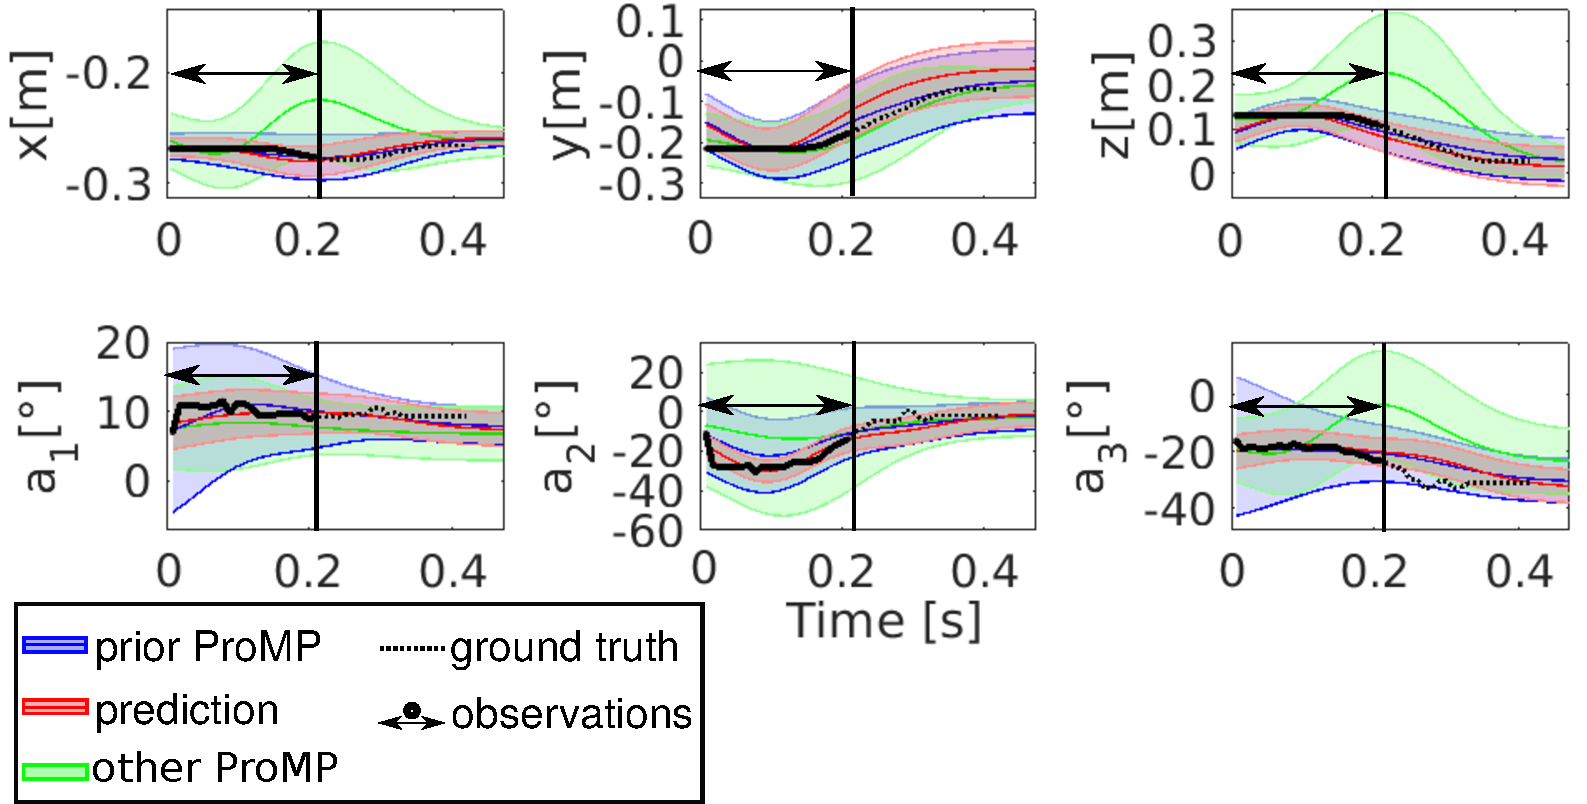
\includegraphics[width=\hsize]{figures/multi.pdf}\\%inferenceHead.pdf}}
	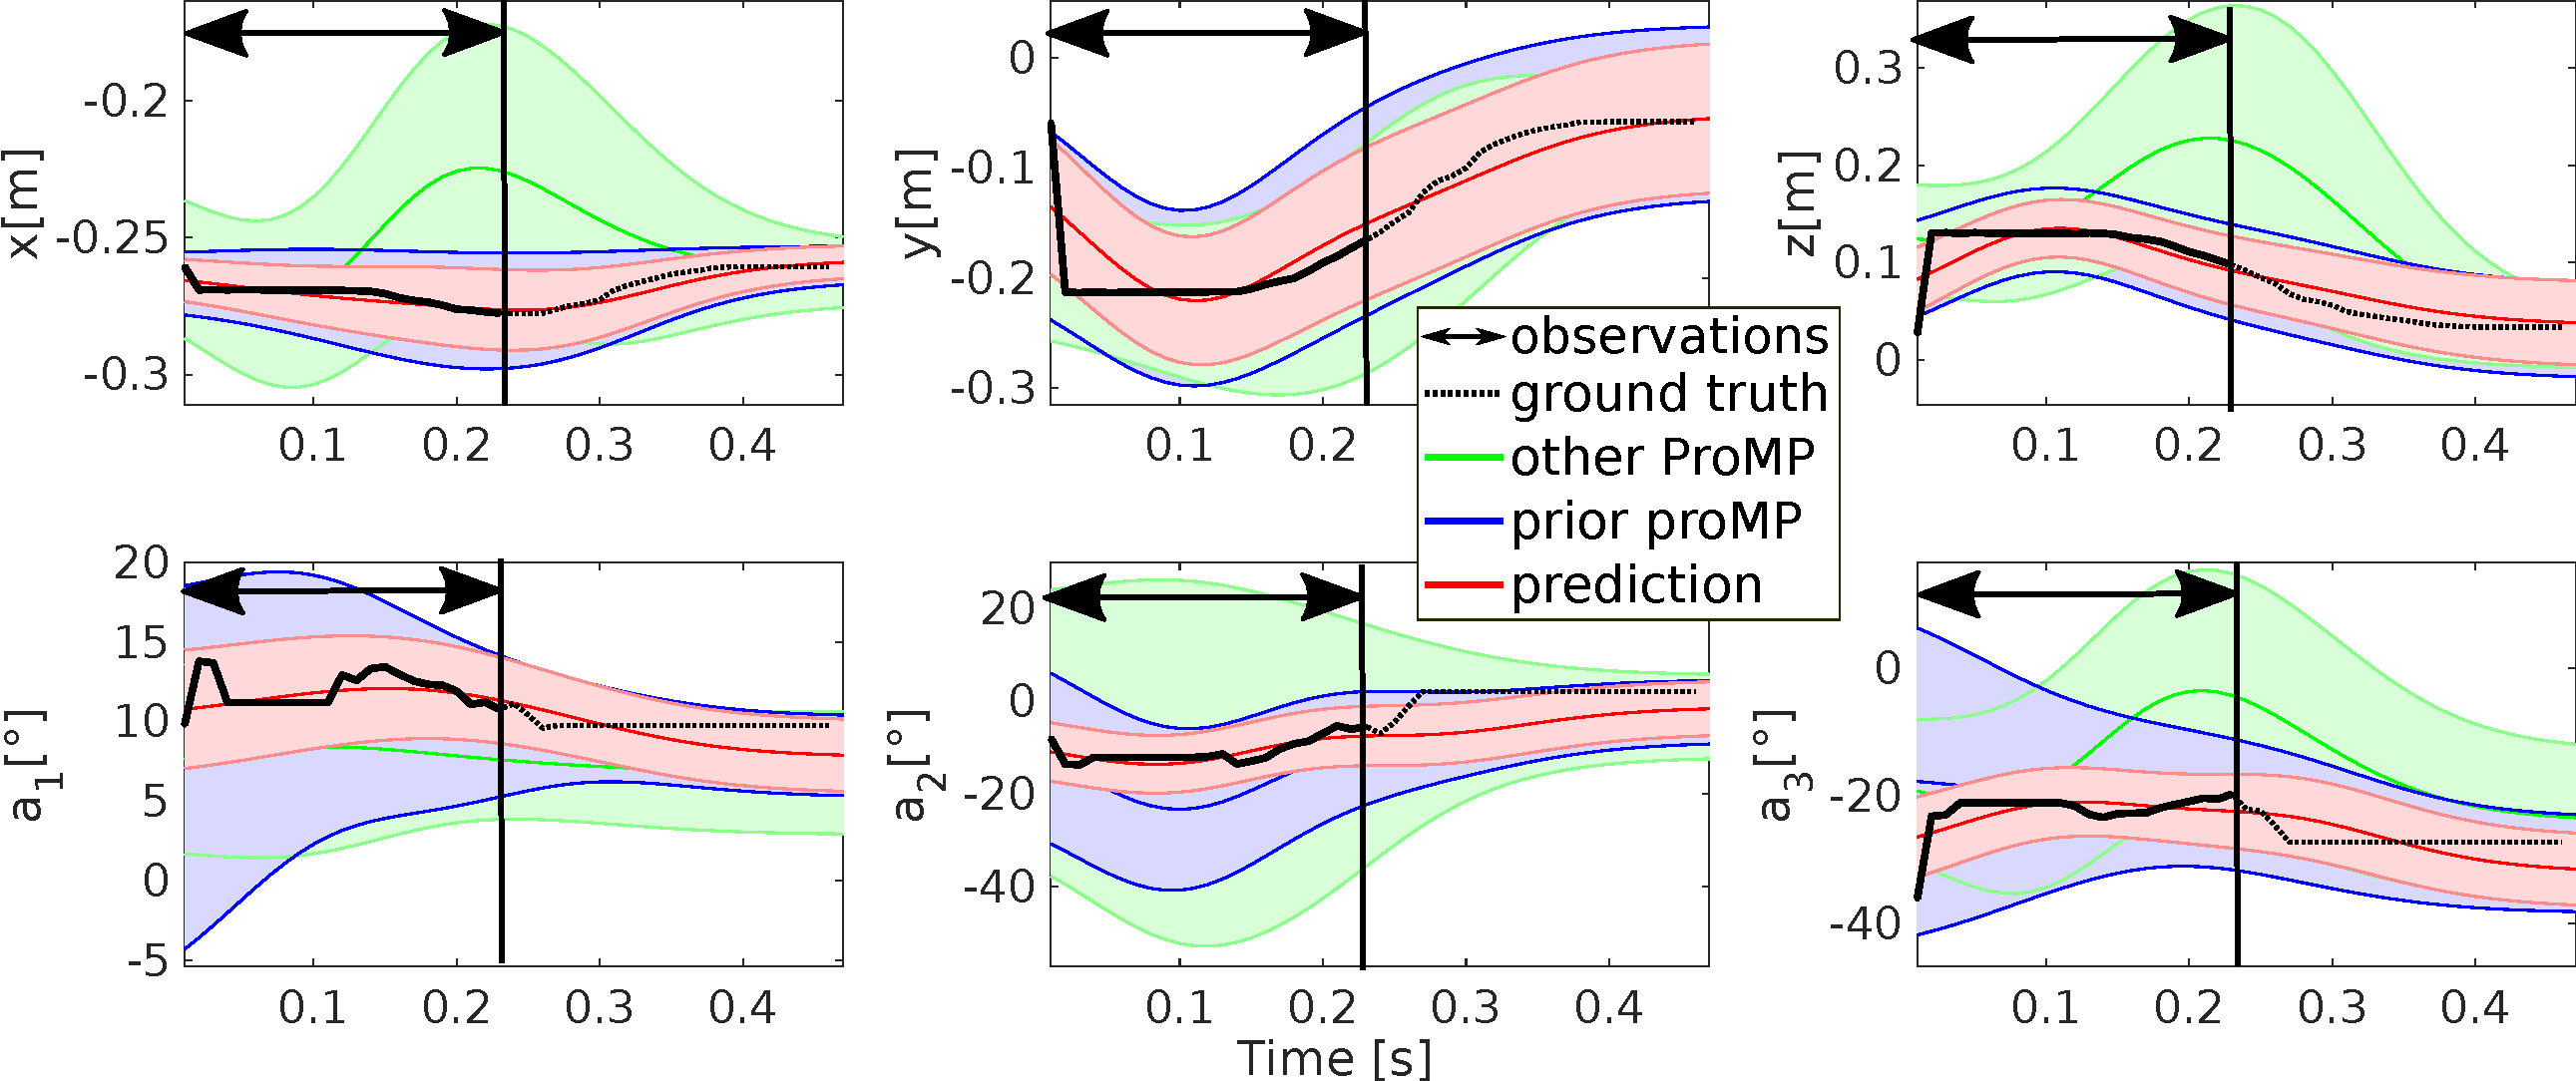
\includegraphics[width=\hsize]{figures/multiN.pdf}
      \caption{Example of position inference from 50\% of the head orientation and the Cartesian position trajectories.\label{fig:infMulti}}
\end{figure} 

Fig.~\ref{fig:infMulti} represents the inference of the Cartesian position trajectory when the robot knows $50\%$ of the trajectory data to achieve and when it uses both visual and physical measurements (black curves). In this example, the inferred trajectory (mean of the red posterior distribution) is close to the trajectory expected by the partner (black dots). To compare this multi-modal prediction with visual or physical prediction only, Fig.~\ref{fig:errInfMulti} and~\ref{fig:predErr} represent all the statistics for each prediction type. Fig.~\ref{fig:errInfMulti}  represents the distance error between the Cartesian position of the expected and the inferred trajectory. Whether with the \textit{model} (in Fig.~\ref{fig:errInfMultiMod}) or the \textit{ML} method (in Fig~\ref{fig:errInfMultiML}), the inference using the Cartesian position measurement only is more accurate than using the multi-modal or the visual-only measurement. The performance of this physical guidance is mainly visible with the \textit{model} method, where the distance error is really short. Thus, the multi-modality guidance did not improve the inference ability of the robot. 

From Fig.~\ref{fig:MultiResult}, we can see the number of ProMP recognition error according to the type of modality used to perform the inference. An interesting result is that by using the \textit{model} method (in Fig.~\ref{fig:predErrMod}), the robot is entirely able to recognize the initiated movement from $70 \%$ of know data, and with the \textit{ML} method, the robot has only done one error from the $38$ trials (which corresponds to $2\%$). Thus, the multi-modal clearly improves the ProMP recognition step of the inference, even though it did not improve the final inferred trajectory precision.

\begin{figure}
  \centering
  \subfloat[With the model.]{\label{fig:errInfMultiMod}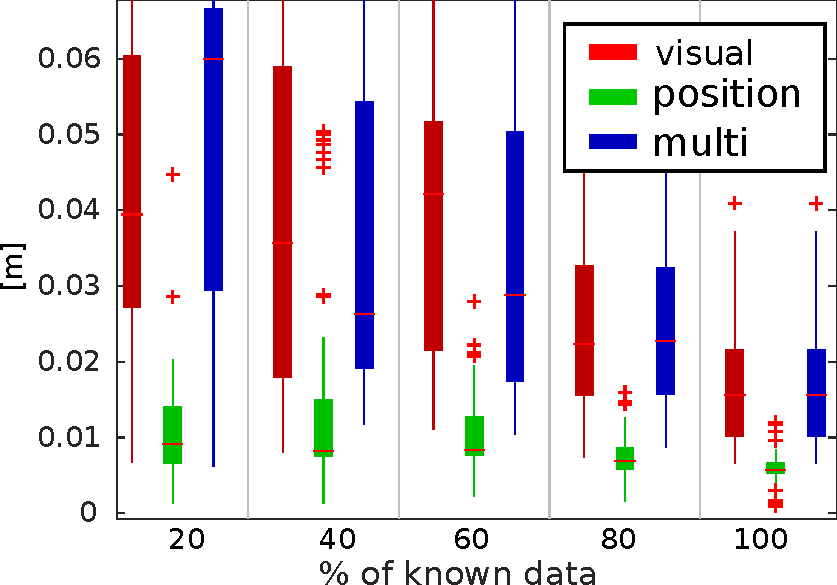
\includegraphics[width=173.5 pt]{figures/globalInfErrMod.pdf}}
    \subfloat[With the Maximum Likelihood.]{\label{fig:errInfMultiML}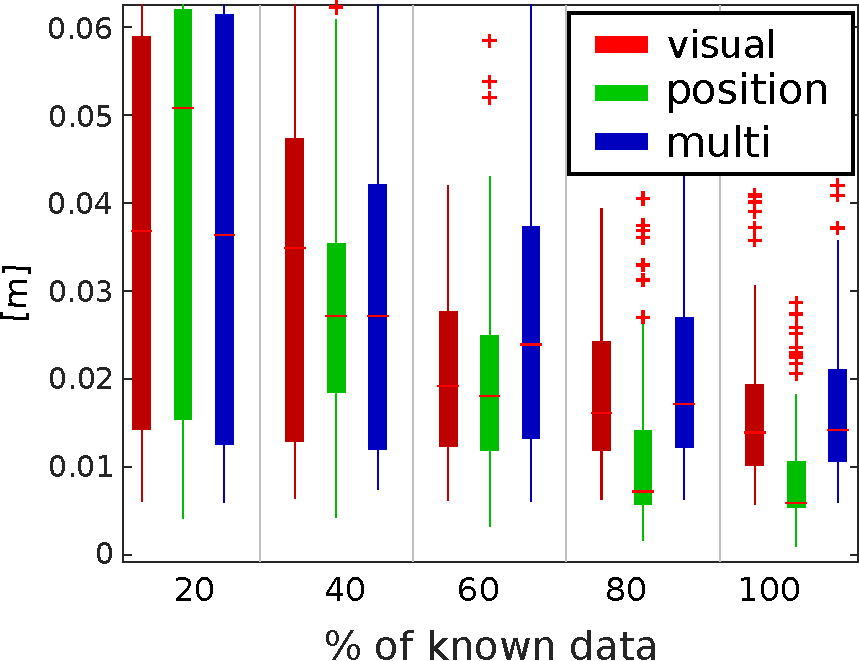
\includegraphics[width=173.5 pt]{figures/globalInfErrML.pdf}}    
\caption{\label{fig:errInfMulti} Inference error of the Cartesian position: average$ |X_{des} - \hat{X}|$ \\ according to modality used.}
\end{figure} 

\begin{figure}
  \centering
  \subfloat[With model.]{\label{fig:predErrMod}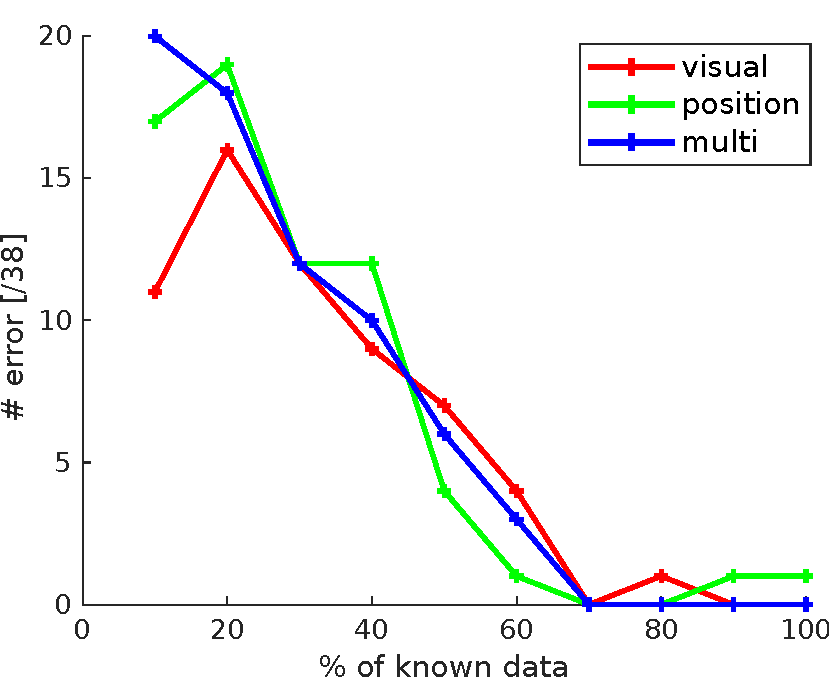
\includegraphics[width=173.5 pt]{figures/globalNbErrMod.pdf}}
    \subfloat[With Maximum Likelihood.]{\label{fig:predErrML}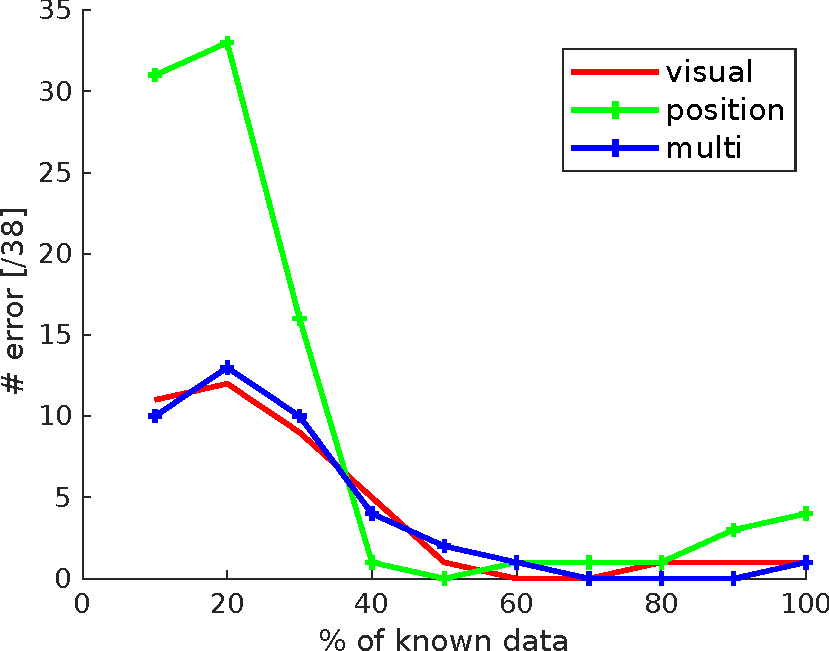
\includegraphics[width=173.5 pt]{figures/globalNbErrML.pdf}}
    %errorPriorVSinfV3
\caption{\label{fig:predErr}Prediction error according to modality used.}
  \label{fig:MultiResult}
\end{figure}

\section{Conclusions}
\label{sec:ccl}
%\small{\normalsize
%In this paper, we present a multi-modal method that allows the humanoid iCub robot to predict the trajectory that should be followed according to the user's intent, using physical or visual measurements.
%Results show that the partner's head orientation is a sufficient measurement to recognize the trajectory to follow, even when the initial and final positions are the same. This is a significant improvement compared to our previous work. However, results also show that the robot cannot use the partner's head orientation to adapt accurately the recognized the ProMP distribution to the early-trajectory. One reason is that this measurement is not accurate. We could record more head orientation trajectories to improve this inference ability, or to change the program from which we retrieve the head orientation. 
%To conclude, physical guidance has the advantages to adapt the recognized trajectory to the early-observations, and to predict correctly the trajectory duration, which improves the recognition skill. Visual guidance is easily usable and to recognize the correct trajectory, even when trajectories are identical at the beginning of the movement.
%In future works, we will study the human preference for use between these modalities. We will also test if the simultaneous use of many modalities at the same time can improve this inference skill.
This paper presents a multi-modal method for robots to predict the partner's intended trajectory during HRI using haptic and/or gaze cues. 
We tested our system with the humanoid iCub collaborating with a human partner in a task where the robot has to grasp an object using different trajectories. 
The human physically interacts with the robot's arm to start an action and/or uses his directional gaze to guide the robot.
We build on our previous work~\cite{oriane2017}, where elementary actions are represented by Probabilistic Movement Primitives that enable prediction of goals from early observations. During physical guidance, the robot uses the haptic information to recognize the current action, then it is able to accurately predict the goal, the future intended trajectory and its duration. 
A limitation of previous inference method is that the robot is not able to determine which movement primitive to follow when the early-observations are ambiguous, \textit{i.e.}, identical to more than one primitive. In that case, the visual guidance is used to identify the correct movement primitive.
While during the visual guidance, the same prediction is done using the directional gaze, approximated here by the head orientation. The association between gaze cues and robot primitives is done by a multi-modal learning phase.
The visual modality has two main advantages: first, it does not require the partner to physically touch the robot to start his intended movement; second, it provides a faster recognition of the action primitive if compared with physical signals. However, results show that by using the visual instead of the physical guidance, the performance of the inference decreases slightly (around $1.5cm$).
A limit of this modality is the accuracy of the gaze estimation. To improve it, we have many possibilities: use the Kinect to have more relevant data; use another head recognition software instead of Intraface; or use the  Xsens 3D tracking. 
%The last possibility is the most promising. 
It is also possible to add another \textit{"no-human"} modality to even surpass human inference skills, by guiding the robot from a watch that contains sensors to detect the human partner's arm pose and to use this pose to learn and recognize ProMPs. 

Regarding the inference using multi-modal measurements, results show that by adding the visual recognition in addition to the physical recognition, it did not improve the accuracy of the inferred trajectory (\textit{i.e.}, it did not improve the posterior distribution computation), but it improves the ProMP recognition (\textit{i.e.}, it improves the first step of the inference that consists on recognizing which movement the robot has to execute among the one it has learned). Thus, to have the better inference skills, we should use the multi-modal guidance to allow robots to recognize the movement/action to perform, and then we should use the haptic guidance to improve the movement precision according to the early measurements. However, the multi-modal guidance currently requires to use two human partners (one in front of the robot to guide it with his/her head and the other one to guide it physically) or to perform the guidance type one after the other. The utilization of the Xsens is a good way to improve this study because one partner will be able to guide physically and visually the partner at the same time, hence in a more natural way.

In future work, we will also study the human preference for the use between the haptic and visual guidance modes. 

%\par}
\subsubsection*{Acknowledgments.} 
%\small{\normalsize

The authors wish to thank Olivier Rochel, Alexandros Paraschos, Marco Ewerton, Waldez Azevedo Gomes Junior and Pauline Maurice for their help and feedbacks.

%the IIT researchers of the CoDyCo
%project for their support with iCub, Olivier Rochel, Alexandros Paraschos and Macro Ewerton for their help with this work and Pauline Maurice for her pertinent feedback.
%\section{The References Section}\label{references}
%
%In order to permit cross referencing within LNCS-Online, and eventually
%between different publishers and their online databases, LNCS will,
%from now on, be standardizing the format of the references. This new
%feature will increase the visibility of publications and facilitate
%academic research considerably. Please base your references on the
%examples below. References that don't adhere to this style will be
%reformatted by Springer. You should therefore check your references
%thoroughly when you receive the final pdf of your paper.
%The reference section must be complete. You may not omit references.
%Instructions as to where to find a fuller version of the references are
%not permissible.
%
%We only accept references written using the latin alphabet. If the title
%of the book you are referring to is in Russian or Chinese, then please write
%(in Russian) or (in Chinese) at the end of the transcript or translation
%of the title.
%
%The following section shows a sample reference list with entries for
%journal articles \cite{jour}, an LNCS chapter \cite{lncschap}, a book
%\cite{book}, proceedings without editors \cite{proceeding1} and
%\cite{proceeding2}, as well as a URL \cite{url}.
%Please note that proceedings published in LNCS are not cited with their
%full titles, but with their acronyms!
\begin{thebibliography}{4}
\providecommand{\url}[1]{\texttt{#1}}
\providecommand{\urlprefix}{URL }

\bibitem{anzalone2015evaluating}
Anzalone, S.M., Boucenna, S., Ivaldi, S., Chetouani, M.: Evaluating the
  engagement with social robots. I.J. of Social Robotics
  7(4),  465--478 (2015)

\bibitem{bader2009multimodal}
Bader, T., Vogelgesang, M., Klaus, E.: Multimodal integration of natural gaze
  behavior for intention recognition during object manipulation. In:
  PIC on Multimodal interfaces.
  pp. 199--206. ACM (2009)

\bibitem{baluja1994non}
Baluja, S., Pomerleau, D.: Non-intrusive gaze tracking using artificial neural
  networks. In: Advances in NIPS. pp. 753--760
  (1994)

\bibitem{boucenna2014robot}
Boucenna, S., Gaussier, P., Andry, P., Hafemeister, L.: A robot learns the
  facial expressions recognition and face/non-face discrimination through an
  imitation game. International Journal of Social Robotics  6(4),  633--652
  (2014)

\bibitem{bretherton1991intentional}
Bretherton, I.: Intentional communication and the development of an
  understanding of mind. Children's theories of mind: Mental states and social
  understanding pp. 49--75 (1991)

\bibitem{castellano2009detecting}
Castellano, G., Pereira, A., Leite, I., Paiva, A., McOwan, P.W.: Detecting user
  engagement with a robot companion using task and social interaction-based
  features. In: PIC on Multimodal
  interfaces. pp. 119--126. ACM (2009)

\bibitem{oriane2017}
Dermy, O., Paraschos, A., Ewerton, M., Peters, J., Charpillet, F., Ivaldi, S.:
  Prediction of intention during interaction with icub with probabilistic
  movement primitives, Frontiers in robotics and AI (2017)

\bibitem{dillmann2004armar}
Dillmann, R., Becher, R., Steinhaus, P.: {ARMAR} II-a learning and cooperative
  multimodal humanoid robot system. International Journal of Humanoid Robotics
  1(01),  143--155 (2004)

\bibitem{Dragan2013rss}
Dragan, A., Srinivasa, S.: Generating legible motion. In: Proceedings of
  Robotics: Science and Systems. Berlin, Germany (June 2013)

\bibitem{dragan2014integrating}
Dragan, A., Srinivasa, S.: Integrating human observer inferences into robot
  motion planning. Autonomous Robots  37(4),  351--368 (2014)

\bibitem{ferrer2014bayesian}
Ferrer, G., Sanfeliu, A.: Bayesian human motion intentionality prediction in
  urban environments. Pattern Recognition Letters  44,  134--140 (2014)

\bibitem{HOFFMAN2006299}
Hoffman, M.W., Grimes, D.B., Shon, A.P., Rao, R.P.: A probabilistic model of
  gaze imitation and shared attention. Neural Networks  19(3),  299 -- 310
  (2006)

\bibitem{huang2016anticipatory}
Huang, C.M., Mutlu, B.: Anticipatory robot control for efficient human-robot
  collaboration. In: HRI, 2016 pp. 83--90

\bibitem{ishii2011combining}
Ishii, R., Shinohara, Y., Nakano, T., Nishida, T.: Combining multiple types of
  eye-gaze information to predict user's conversational engagement. In: 2nd
  workshop on eye gaze on intelligent human machine interaction (2011)

\bibitem{ivaldi2017towards}
Ivaldi, S., Lefort, S., Peters, J., Chetouani, M., Provasi, J., Zibetti, E.:
  Towards engagement models that consider individual factors in HRI. Int. J. of Social
  Robotics  9,  63--86 (2017)

\bibitem{kim2017collaborative}
Kim, J., Banks, C.J., Shah, J.A.: Collaborative planning with encoding of
  users' high-level strategies. In: AAAI (2017)

\bibitem{kozima2001robot}
Kozima, H., Yano, H.: A robot that learns to communicate with human caregivers.
  In: Proceedings of the First International Workshop on Epigenetic Robotics.
  pp. 47--52 (2001)

\bibitem{ma2005eye}
Ma, C., Prendinger, H., Ishizuka, M.: Eye movement as an indicator of users'
  involvement with embodied interfaces at the low level. In: Proc. AISB
 pp.  136--143 (2005)

\bibitem{meltzoff2007eyes}
Meltzoff, A.N., Brooks, R.: Eyes wide shut: The importance of eyes in infant
  gaze following and understanding other minds. Gaze following: Its development
  and significance, ed. R. Flom, K. Lee \& D. Muir. Erlbaum.[EVH]  (2007)

\bibitem{mitsugami2005robot}
Mitsugami, I., Ukita, N., Kidode, M.: Robot navigation by eye pointing. Lecture
  notes in computer science  3711,  256 (2005)

\bibitem{paraschos2013probabilistic}
Paraschos, A., Daniel, C., Peters, J.R., Neumann, G.: Probabilistic movement
  primitives. In: NIPS pp.
  2616--2624 (2013)

\bibitem{chaandar2016bayesian}
H.C. Ravichandar, H., Kumar, A., Dani, A.: Bayesian human intention
  inference through multiple model filtering with gaze-based priors. In:
  Information Fusion (FUSION) pp.
  2296--2302. IEEE (2016)

\bibitem{timm2011accurate}
Timm, F., Barth, E.: Accurate eye centre localisation by means of gradients.
  Visapp  11,  125--130 (2011)

\bibitem{traver2000making}
Traver, V.J., del Pobil, A.P., P{\'e}rez-Francisco, M.: Making service robots
  human-safe. In: Proceedings.(IROS 2000) on. vol.~1, pp. 696--701.  IEEE (2000)

\bibitem{walker1997infants}
Walker-Andrews, A.S.: Infants' perception of expressive behaviors:
  differentiation of multimodal information. Psychological bulletin  121(3),
  437 (1997)

\bibitem{wang2012probabilistic}
Wang, Z., Deisenroth, M.P., Amor, H.B., Vogt, D., Sch{\"o}lkopf, B., Peters,
  J.: Probabilistic modeling of human movements for intention inference. In:
  Robotics: Science and Systems. (2012)

\bibitem{weser2006multimodal}
Weser, M., Westhoff, D., Huser, M., Zhang, J.: Multimodal people tracking and
  trajectory prediction based on learned generalized motion patterns. In: Int. Conf. Multisensor Fusion and Integration for Intelligent Systems, pp. 541--546 (2006). 

\bibitem{XiongD13}
Xiong, X., {De la Torre}, F.: Supervised descent method and its applications to
  face alignment. In: IEEE CVPR (2013)

\end{thebibliography}
%\bibliographystyle{splncs03}
%\bibliography{soa}
%\par}
%
%\section{BibTeX Entries}
%
%The correct BibTeX entries for the Lecture Notes in Computer Science
%volumes can be found at the following Website shortly after the
%publication of the book:
%\url{http://www.informatik.uni-trier.de/~ley/db/journals/lncs.html}

%\begin{thebibliography}{4}
%\providecommand{\url}[1]{\texttt{#1}}
%\providecommand{\urlprefix}{URL }
%
%\end{thebibliography}


%
%\bibitem{jour} Smith, T.F., Waterman, M.S.: Identification of Common Molecular
%Subsequences. J. Mol. Biol. 147, 195--197 (1981)
%
%\bibitem{lncschap} May, P., Ehrlich, H.C., Steinke, T.: ZIB Structure Prediction Pipeline:
%Composing a Complex Biological Workflow through Web Services. In: Nagel,
%W.E., Walter, W.V., Lehner, W. (eds.) Euro-Par 2006. LNCS, vol. 4128,
%pp. 1148--1158. Springer, Heidelberg (2006)
%
%\bibitem{book} Foster, I., Kesselman, C.: The Grid: Blueprint for a New Computing
%Infrastructure. Morgan Kaufmann, San Francisco (1999)
%
%\bibitem{proceeding1} Czajkowski, K., Fitzgerald, S., Foster, I., Kesselman, C.: Grid
%Information Services for Distributed Resource Sharing. In: 10th IEEE
%International Symposium on High Performance Distributed Computing, pp.
%181--184. IEEE Press, New York (2001)
%
%\bibitem{proceeding2} Foster, I., Kesselman, C., Nick, J., Tuecke, S.: The Physiology of the
%Grid: an Open Grid Services Architecture for Distributed Systems
%Integration. Technical report, Global Grid Forum (2002)
%
%\bibitem{url} National Center for Biotechnology Information, \url{http://www.ncbi.nlm.nih.gov}
%
%\end{thebibliography}

%
%\section*{Appendix: Springer-Author Discount}
%
%LNCS authors are entitled to a 33.3\% discount off all Springer
%publications. Before dropping an order, the author should send an email, 
%giving full details of his or her Springer publication,
%to \url{orders-HD-individuals@springer.com} to obtain a so-called token. This token is a
%number, which must be entered when placing an order via the Internet, in
%order to obtain the discount.
%
%\section{Checklist of Items to be Sent to Volume Editors}
%Here is a checklist of everything the volume editor requires from you:
%
%
%\begin{itemize}
%\settowidth{\leftmargin}{{\Large$\square$}}\advance\leftmargin\labelsep
%\itemsep8pt\relax
%\renewcommand\labelitemi{{\lower1.5pt\hbox{\Large$\square$}}}
%
%\item The final \LaTeX{} source files
%\item A final PDF file
%\item A copyright form, signed by one author on behalf of all of the
%authors of the paper.
%\item A readme giving the name and email address of the
%corresponding author.
%\end{itemize}
\end{document}
